\documentclass[xcolor=x11names, svgnames, rgb]{beamer}

\setbeamertemplate{navigation symbols}{}
\setbeamercolor{block title}{bg=blue!40}
\setbeamercolor{block body}{bg=blue!20}

%% Beamer Layout %%%%%%%%%%%%%%%%%%%%%%%%%%%%%%%%%%
\useoutertheme[subsection=false,shadow]{miniframes}
\useinnertheme{default}
\usefonttheme{serif}
\usepackage{palatino}
\setbeamerfont{title like}{shape=\scshape}
\setbeamerfont{frametitle}{shape=\scshape}
\setbeamercolor*{lower separation line head}{bg=DeepSkyBlue4}
\setbeamercolor*{normal text}{fg=black,bg=white}
\setbeamercolor*{alerted text}{fg=red}
\setbeamercolor*{example text}{fg=black}
\setbeamercolor*{structure}{fg=black}
\setbeamercolor*{palette tertiary}{fg=black,bg=black!10}
\setbeamercolor*{palette quaternary}{fg=black,bg=black!10}
%% END Beamer Layout %%%%%%%%%%%%%%%%%%%%%%%%%%%%%%%%%%%%%%%%%%%%
\usepackage{graphicx}
\usepackage{algpseudocode}
\usepackage{soul}

\usepackage{mathtools}
\newcommand{\defeq}{\vcentcolon=}
\DeclarePairedDelimiter{\paren}{(}{)}

\newcommand{\dec}{\operatorname{dec}}
\newcommand{\poly}{\operatorname{poly}}
\newcommand{\polylog}{\operatorname{polylog}}
\newcommand{\github}{\url{github.com/awestover/Parallel-Partition}}
\newcommand{\defn}[1]       {{\textit{\textbf{\boldmath #1}}}}
\newcommand{\paragraph}[1]{\vspace{0.09in}\noindent{\bf \boldmath #1.}} 
\usepackage{amsmath}
\def\E{\operatorname{\mathbb{E}}}
\usepackage{amssymb}
\usepackage{amsthm}

\newtheorem{proposition}{Proposition}
\newtheorem{defin}{Definition}
\newtheorem{conj}{Conjecture}

\usepackage{hyperref}

\usepackage{tikz,pgfplots}
\usepackage{etoolbox}
%% This makes the colors annoyingly bright, but at least they're easy to distinguish.
\pgfplotsset{
  every  tick/.style={red,}, minor x tick num=1,
  cycle list={teal,every mark/.append style={fill=teal!80!black},mark=*\\%
orange,every mark/.append style={fill=orange!80!black},mark=square*\\%
cyan!60!black,every mark/.append style={fill=cyan!80!black},mark=otimes*\\%
red!70!white,mark=star\\%
lime!80!black,every mark/.append style={fill=lime},mark=diamond*\\%
red,densely dashed,every mark/.append style={solid,fill=red!80!black},mark=*\\%
yellow!60!black,densely dashed,
every mark/.append style={solid,fill=yellow!80!black},mark=square*\\%
black,every mark/.append style={solid,fill=gray},mark=otimes*\\%
blue,densely dashed,mark=star,every mark/.append style=solid\\%
red,densely dashed,every mark/.append style={solid,fill=red!80!black},mark=diamond*\\%
}
}
\pgfplotsset{compat=1.6}


\usepackage{xcolor}
\newcommand{\citefont}[1]{{\tiny \textcolor{Gray}{#1}}}
\setbeamerfont{footnote}{size=\tiny}

\title{The Variable-Processor Cup Game}
\author{Alek Westover}
\institute{Belmont High School}
\date{June 7, 2020}

\begin{document}
 
\frame{\titlepage}

\begin{frame}[c]{$p$-processor cup game on $n$ cups}
  \begin{overprint}
    \onslide<1> 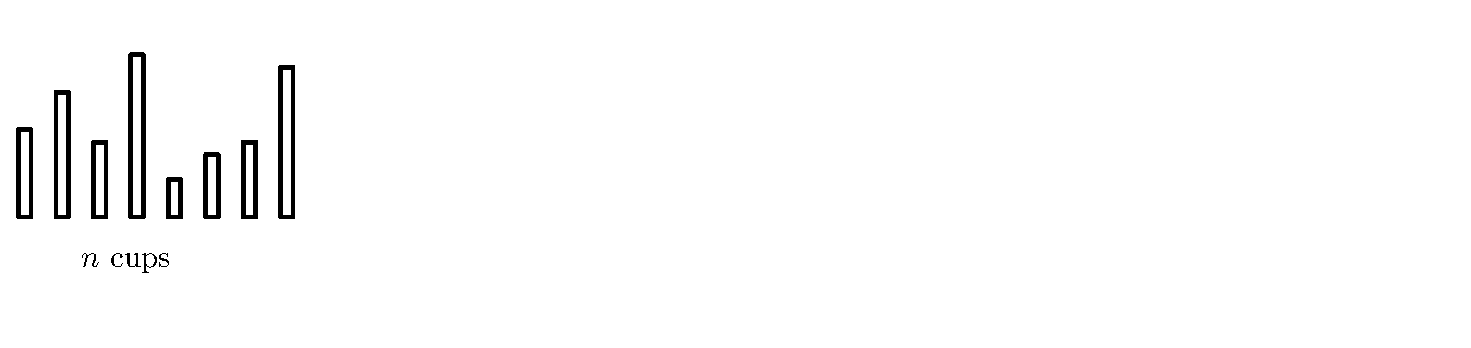
\includegraphics[width=\linewidth]{initDef/initDef0.eps}
    \onslide<2> 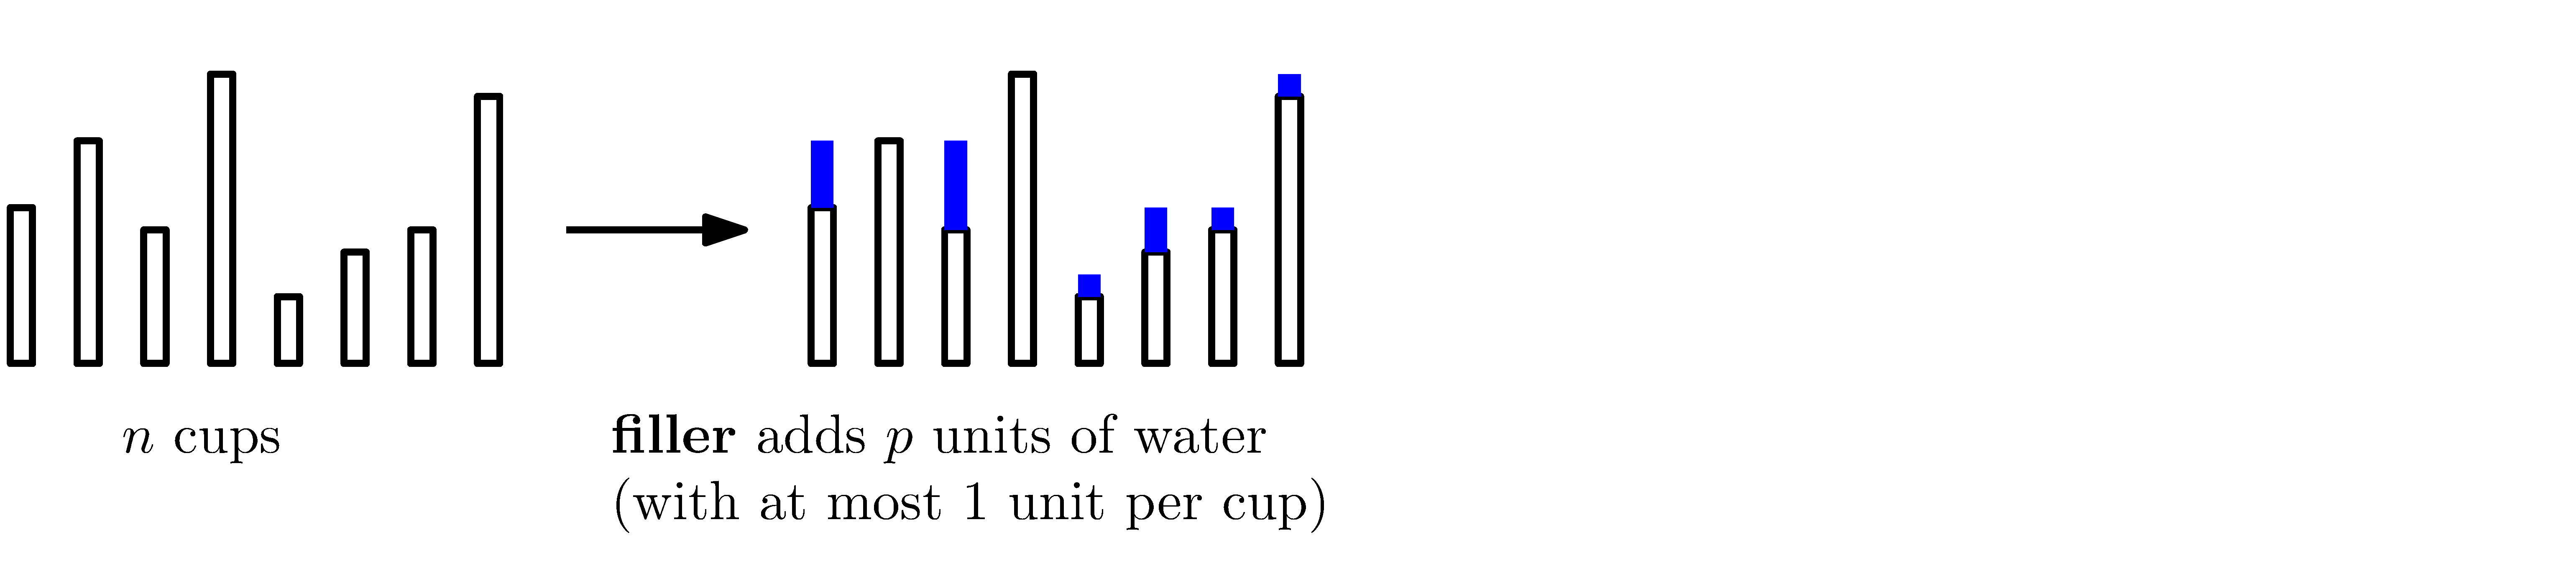
\includegraphics[width=\linewidth]{initDef/initDef1.eps}
    \onslide<3> 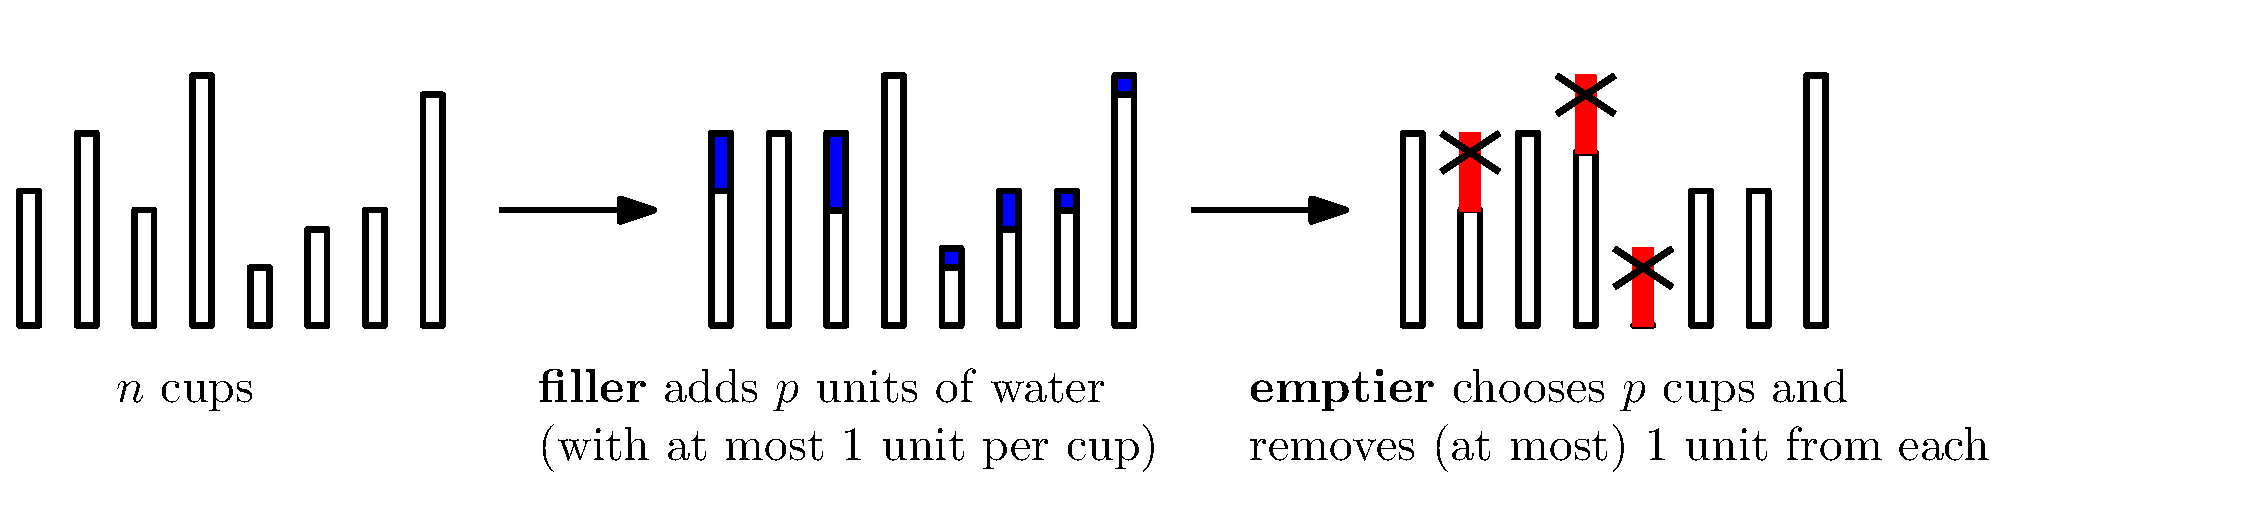
\includegraphics[width=\linewidth]{initDef/initDef2.eps}
    \onslide<4-> 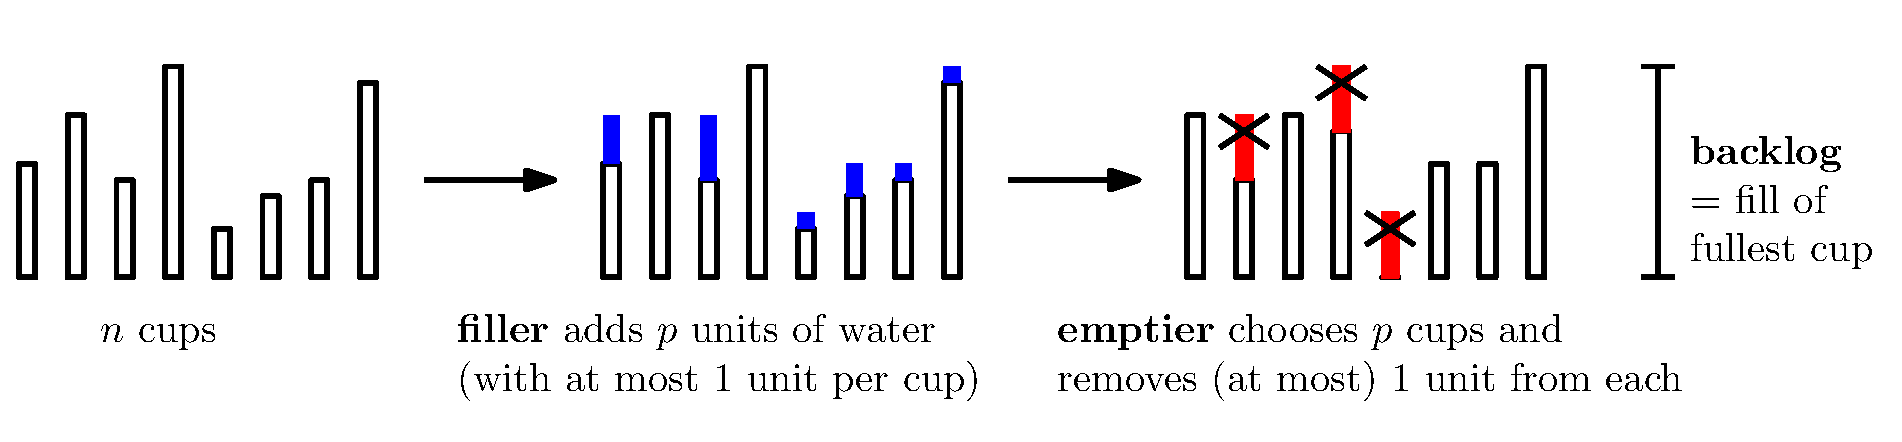
\includegraphics[width=\linewidth]{initDef/initDef3.eps}
  \end{overprint}
  \begin{overprint}
    \onslide<5> {
      \begin{itemize}
        \item filler: wants high backlog 
        \item emptier: wants low backlog
      \end{itemize}
      In this talk we take the side of the filler (so high backlog is good) 
    }
  \end{overprint}
\end{frame}

\begin{frame}[t]{Example Application: Work Scheduling}
  \begin{center}
  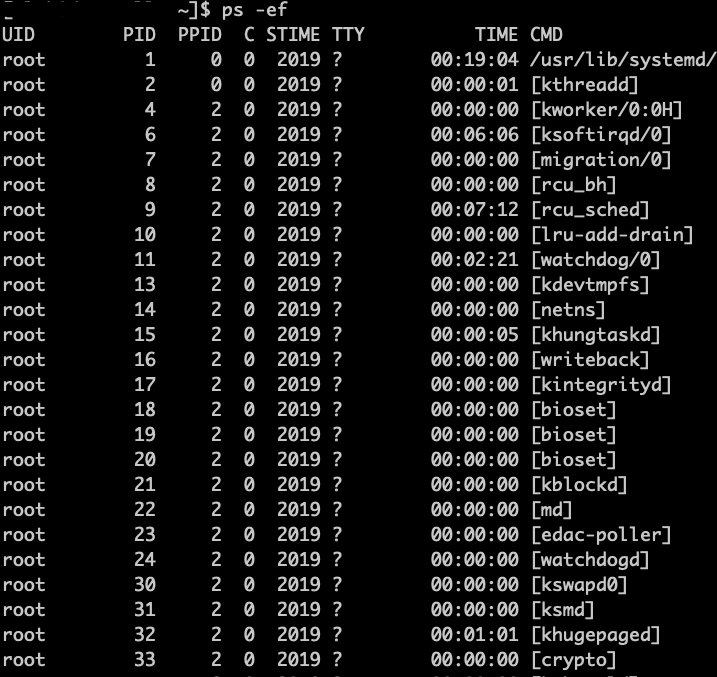
\includegraphics[width=0.36\linewidth]{ps-ef/ps-ef.png}
  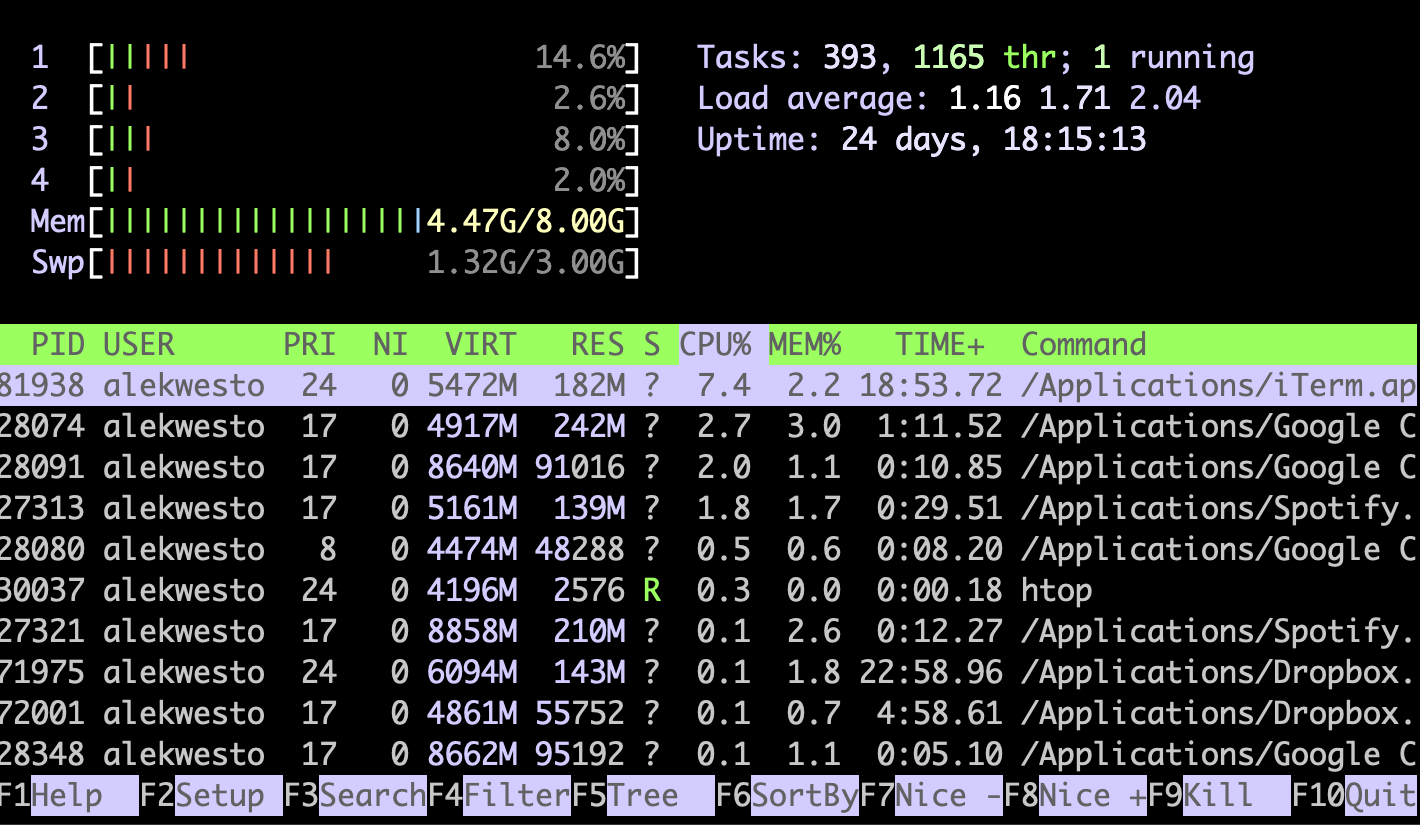
\includegraphics[width=0.62\linewidth]{ps-ef/work_scheduling.png}
  \end{center}
  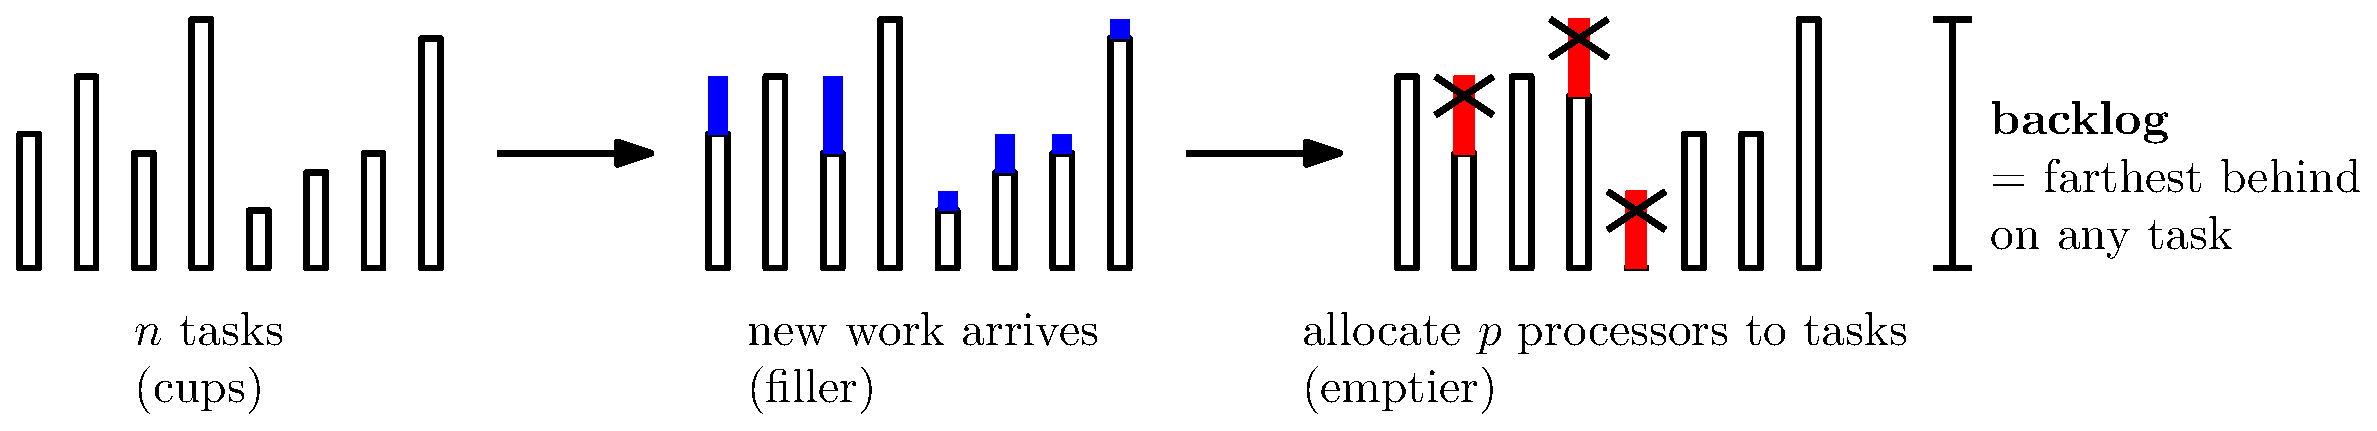
\includegraphics[width=\linewidth]{workScheduling/workScheduling.eps}
\end{frame}

\begin{frame}[t]{Previous Work \footnote{[William Kuszmaul. Achieving optimal backlog in the vanilla multi-processor cup game. SODA, 2020.]}\textsuperscript{,}\footnote{[M. Bender, M. Farach-Colton, and W. Kuszmaul. Achieving optimal backlog in multi-processor cup games. In Proceedings of the 51st Annual ACM Symposium on Theory of Computing (STOC), 2019.]}}
  \defn{Adaptive filler}: can see emptier's actions
  \begin{theorem}
    With an adaptive filler optimal backlog is
    $\Theta(\log n)$.
  \end{theorem}

  \defn{Oblivious filler}: can \textbf{not} see emptier's actions
  \begin{theorem}
    With an oblivious filler optimal backlog is between $\Omega(\log \log n)$ and $O(\log\log n + \log p)$ (with high probability in short games).
  \end{theorem}

\end{frame}

\begin{frame}[t]{This Talk}

  \textbf{Our Question:} What if $p$ can change?
\vspace{1cm}
% Number of processors available to the scheduler could change.
% \vspace{1cm}

  \defn{Variable-Processor Cup Game}: \\
  Each round the filler can change $p$ 

\vspace{1cm}
Modification seems small...
% \vspace{1cm}
% The modification to allow variable resources may seem small. However, we show
% that it drastically changes the game. 
\end{frame}

\begin{frame}[c]{Our Result}
  The variable-processor cup game is \emph{fundamentally different} than the $p$-processor cup game!
\end{frame}

\begin{frame}[t]{Adaptive Filler Lower Bound on Backlog}
  \begin{theorem}
    There is an adaptive filling strategy that achieves
    backlog $$\Omega(n^{1-\epsilon})$$ for any constant $\epsilon >0$ in running-time $$2^{O(\log^2 n)}.$$
  \end{theorem}
\end{frame}
\begin{frame}[t]{Adaptive Filler Lower Bound on Backlog}
  \begin{theorem}
    There is an adaptive filling strategy that achieves backlog $$\Omega(n)$$ in running-time $$O(n!).$$
  \end{theorem}
\end{frame}
\begin{frame}[t]{Upper Bound on Backlog}
  \begin{corollary}
  A greedy emptier never lets backlog exceed $$O(n).$$
  \end{corollary}
  This matches our lower bound!
  \vspace{0.5cm}

  Corollary follows from more general theorem:
  \begin{theorem}
    A greedy emptier maintains the invariant: 
    $$\text{Average fill of $k$ fullest cups } \le 2n-k.$$
  \end{theorem}
\end{frame}
\begin{frame}[t]{Oblivious Filler Lower Bound on Backlog}
  \begin{theorem}
    There is an oblivious filling strategy that achieves backlog
    $$\Omega(n^{1-\epsilon})$$ for constant $\epsilon > 0$ with probability at
    least $1-2^{-\polylog(n)}$ in running time $2^{O(\log^2 n)}$ against a greedy-like emptier.
  \end{theorem}

  \defn{$\Delta$-greedy-like emptier}:

  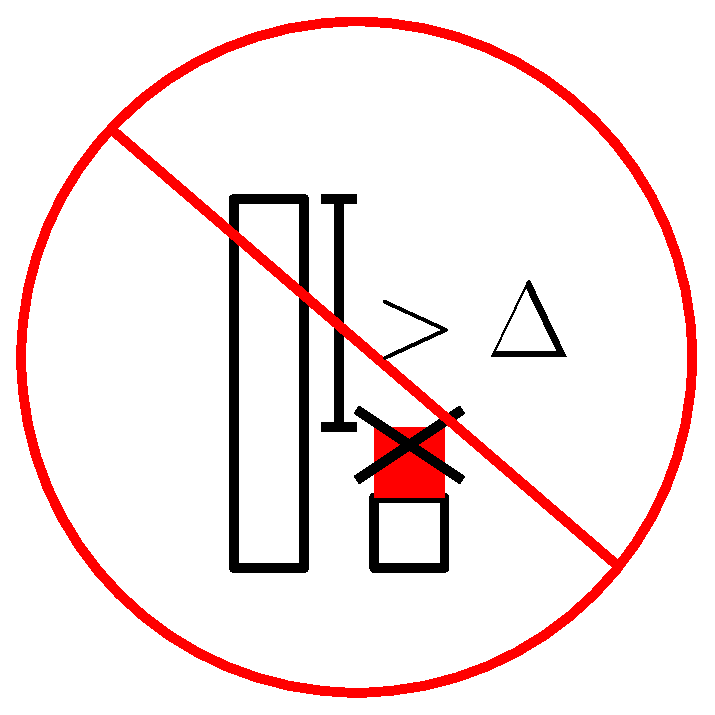
\includegraphics[width=0.22\linewidth]{greedyLike/notallowed.eps}
  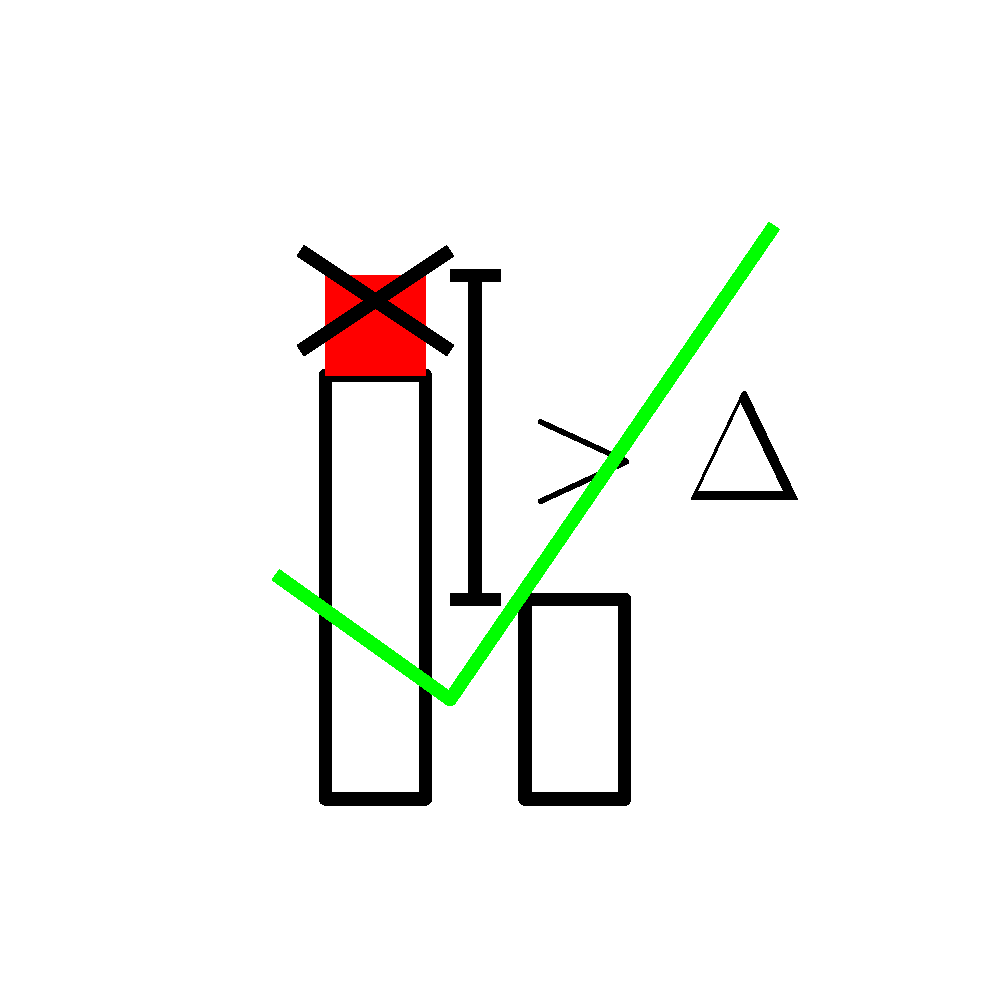
\includegraphics[width=0.22\linewidth]{greedyLike/allowed.eps}
  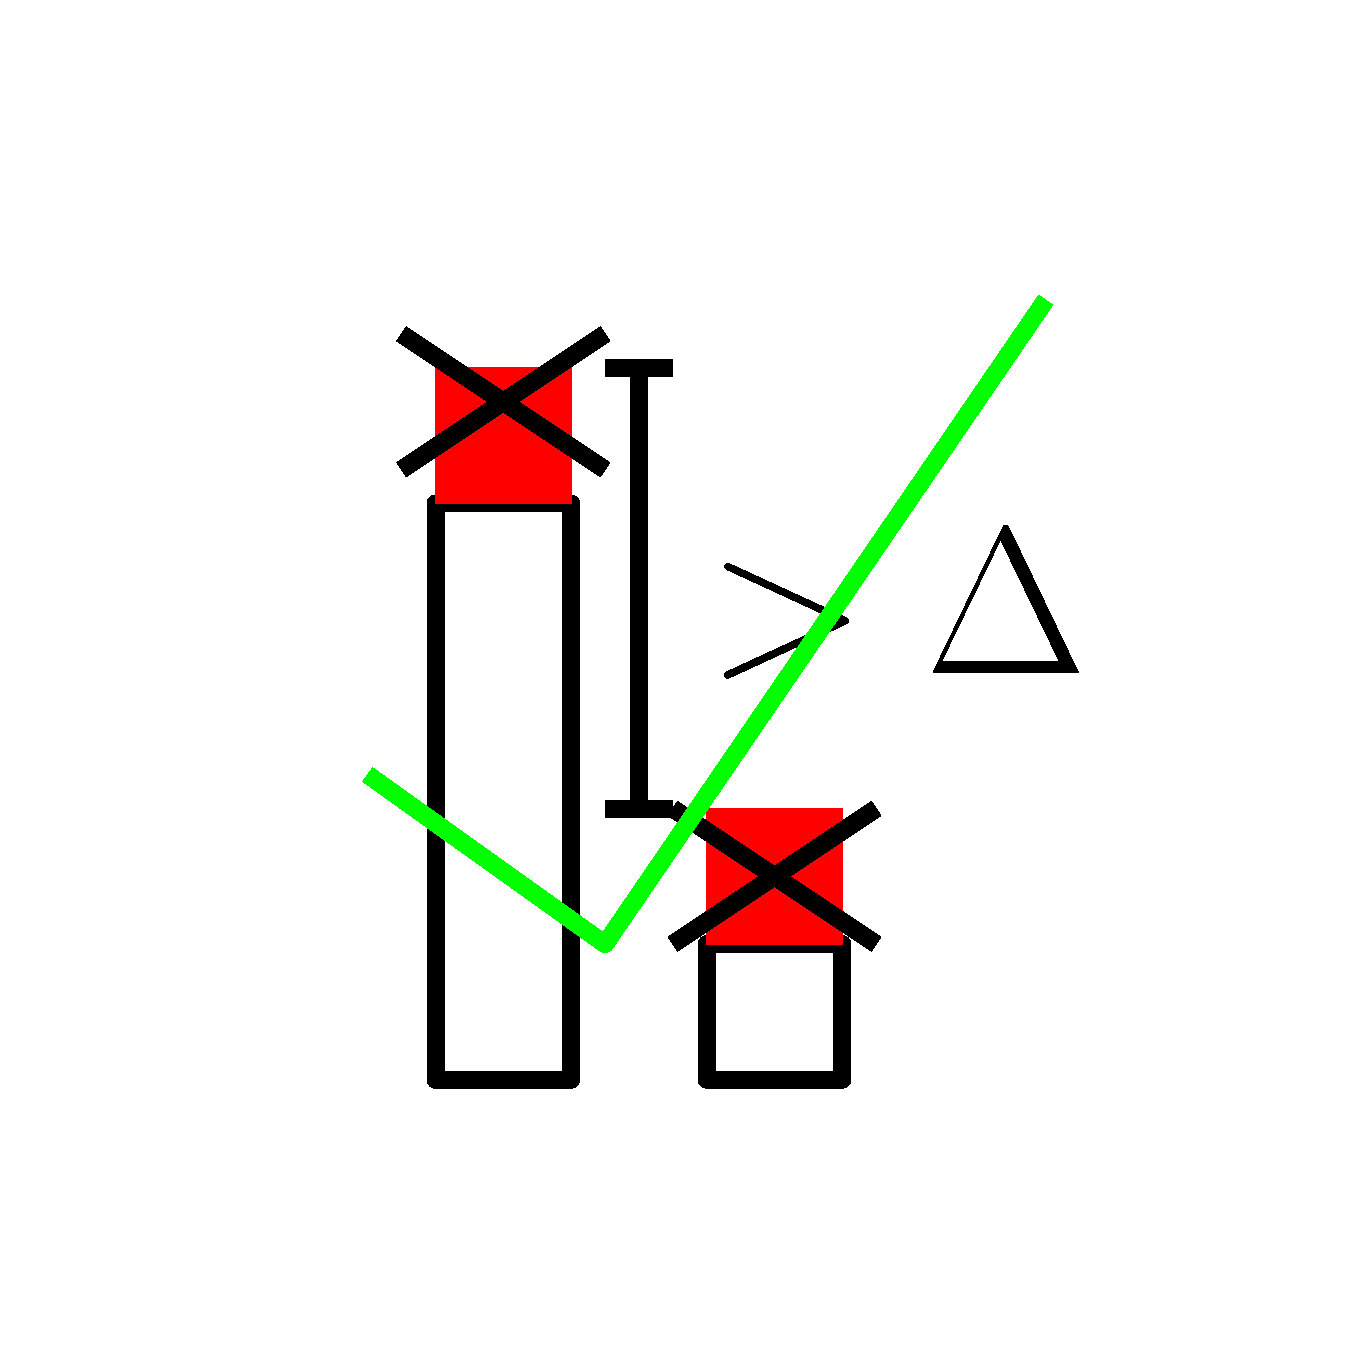
\includegraphics[width=0.22\linewidth]{greedyLike/alsoallowed.eps}
  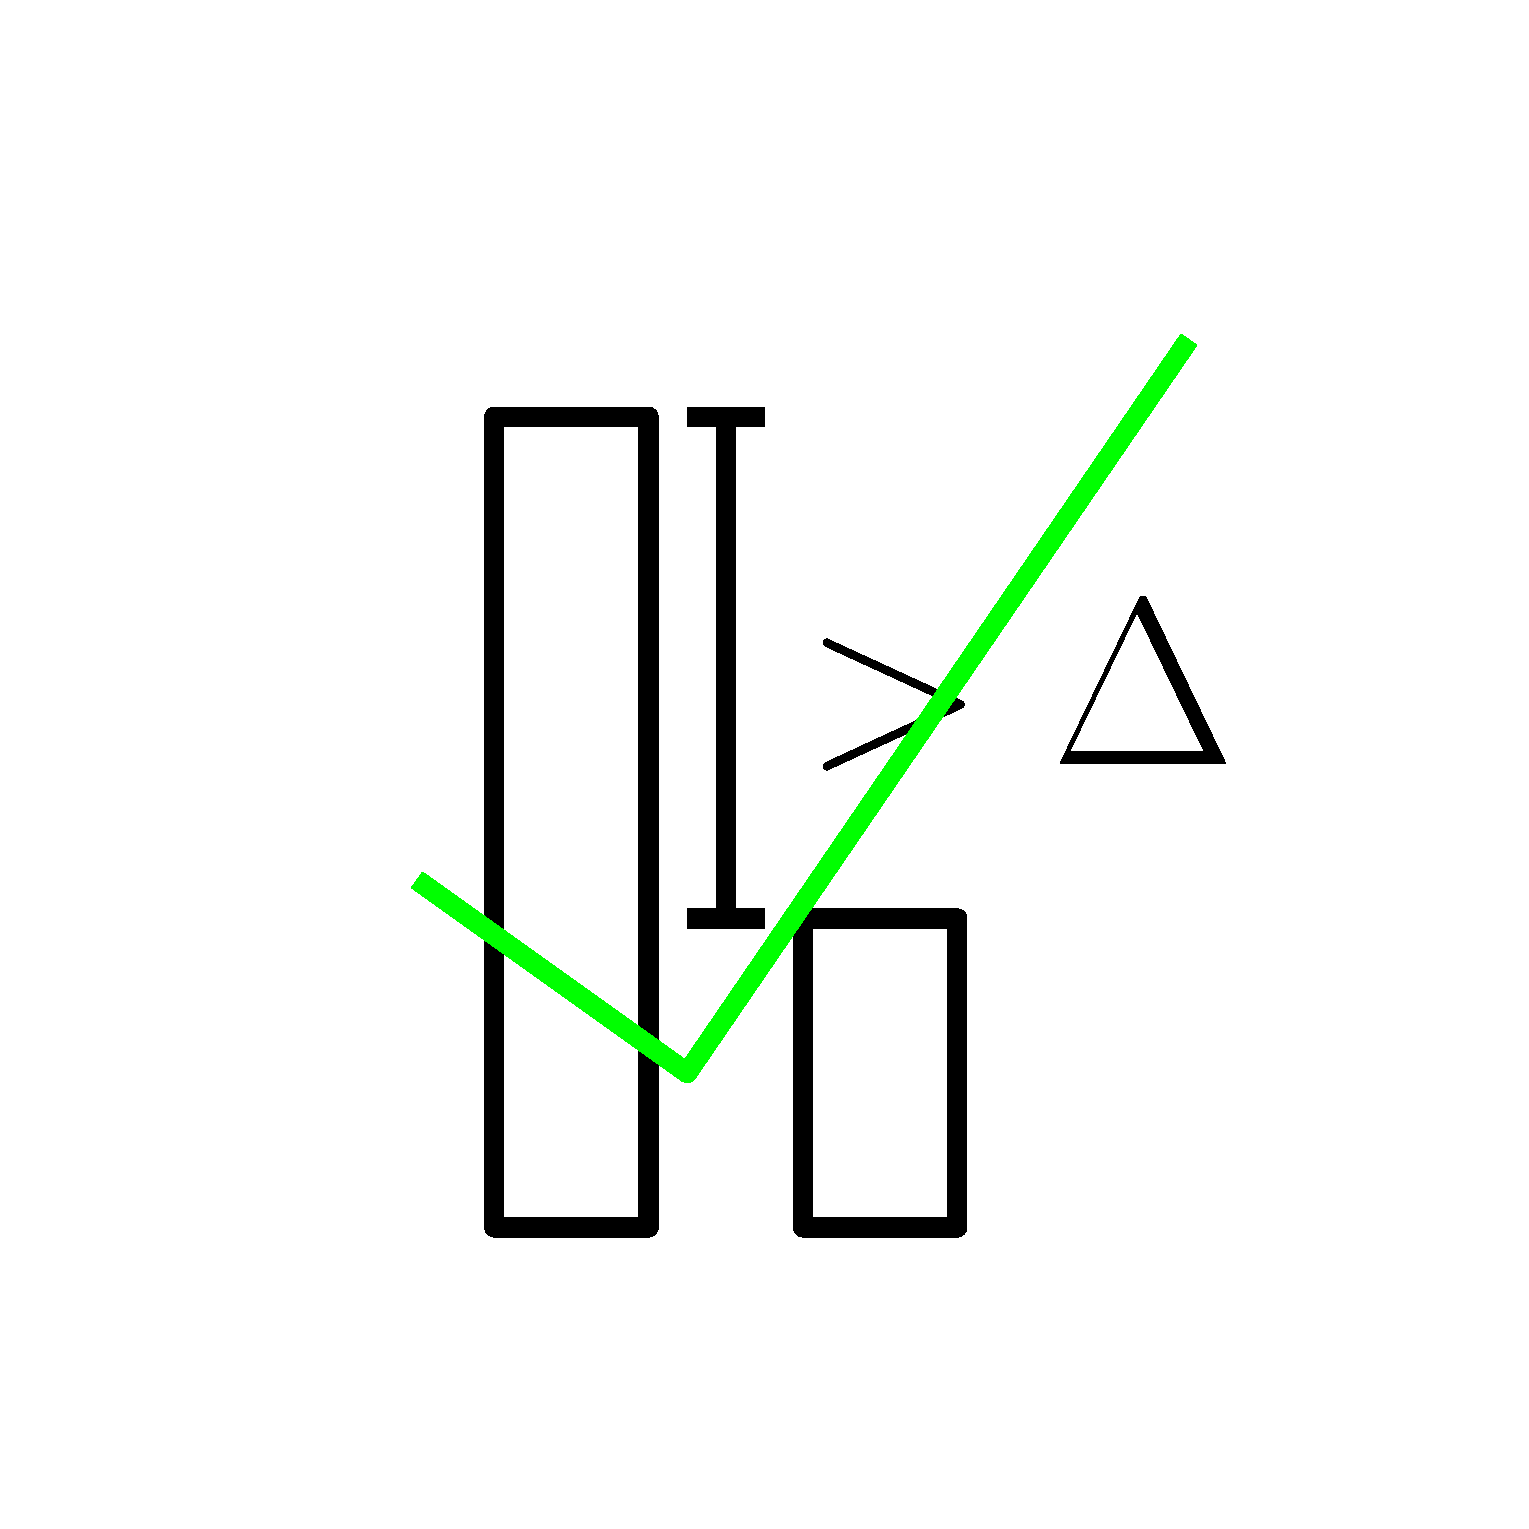
\includegraphics[width=0.22\linewidth]{greedyLike/anotherallowed.eps}

\end{frame}

\begin{frame}[c]{}
\begin{center}
\Huge Adaptive Filler\\ Lower Bound\\ Proof Sketch
\end{center}
\end{frame}

\begin{frame}[t]{Amplification Lemma}
  \begin{lemma}
    Given a strategy $f$ for achieving backlog $f(n)$ on $n$ cups, we can construct a new strategy $f$' that achieves backlog 
    $$f'(n) \ge (1-\delta)\sum_{\ell=0}^L f(n\delta^\ell(1-\delta))$$
    for appropriate parameters $L\in\mathbb{N}, 0<\delta\ll 1/2$.

    If the running time of $f(n)$ is $T(n)$ the running time of $f'(n)$ satisfies
    $$T'(n) \le n\sum_{\ell=0}^L n\delta^\ell T(n\delta^\ell(1-\delta)).$$
  \end{lemma}
\end{frame}

\begin{frame}[t]{Proof Meta-Structure}
  \begin{itemize}
    \item $A$ starts as the $\delta n$ fullest cups, $B$ as the $(1-\delta)n$ other cups.
    \item Repeatedly apply $f$ to $B$ and swap generated cup into $A$. 
    \item Decrease $p$, recurse on $A$.
  \end{itemize} 
  \vspace{0.5cm}
  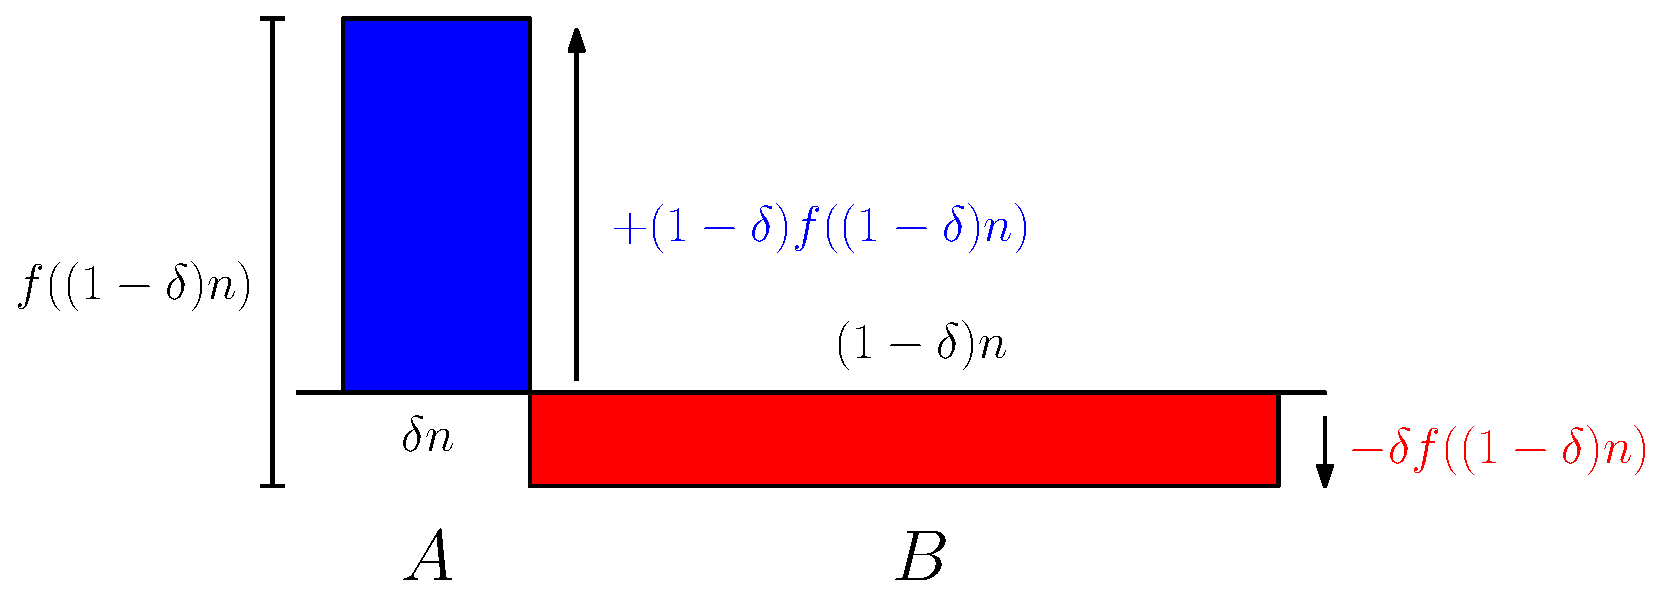
\includegraphics[width=\linewidth]{amplificationImgs/delta_one_minus_delta.eps}
\end{frame}

\begin{frame}[t]{Amplification Lemma Proof Sketch}
  \begin{overprint}
    \onslide<1> 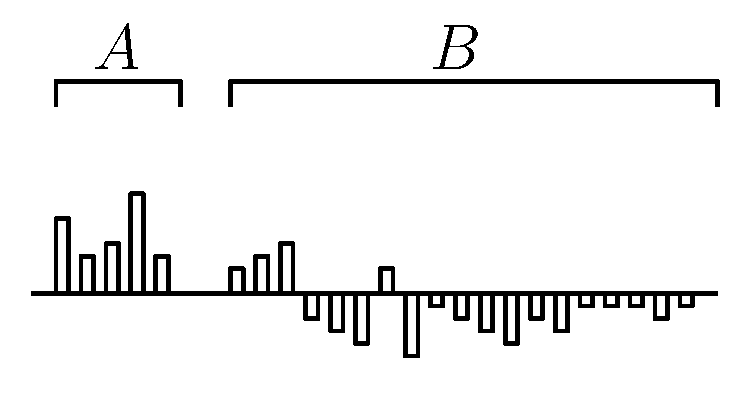
\includegraphics[width=\linewidth]{amppf/ani0.eps}
    \onslide<2> 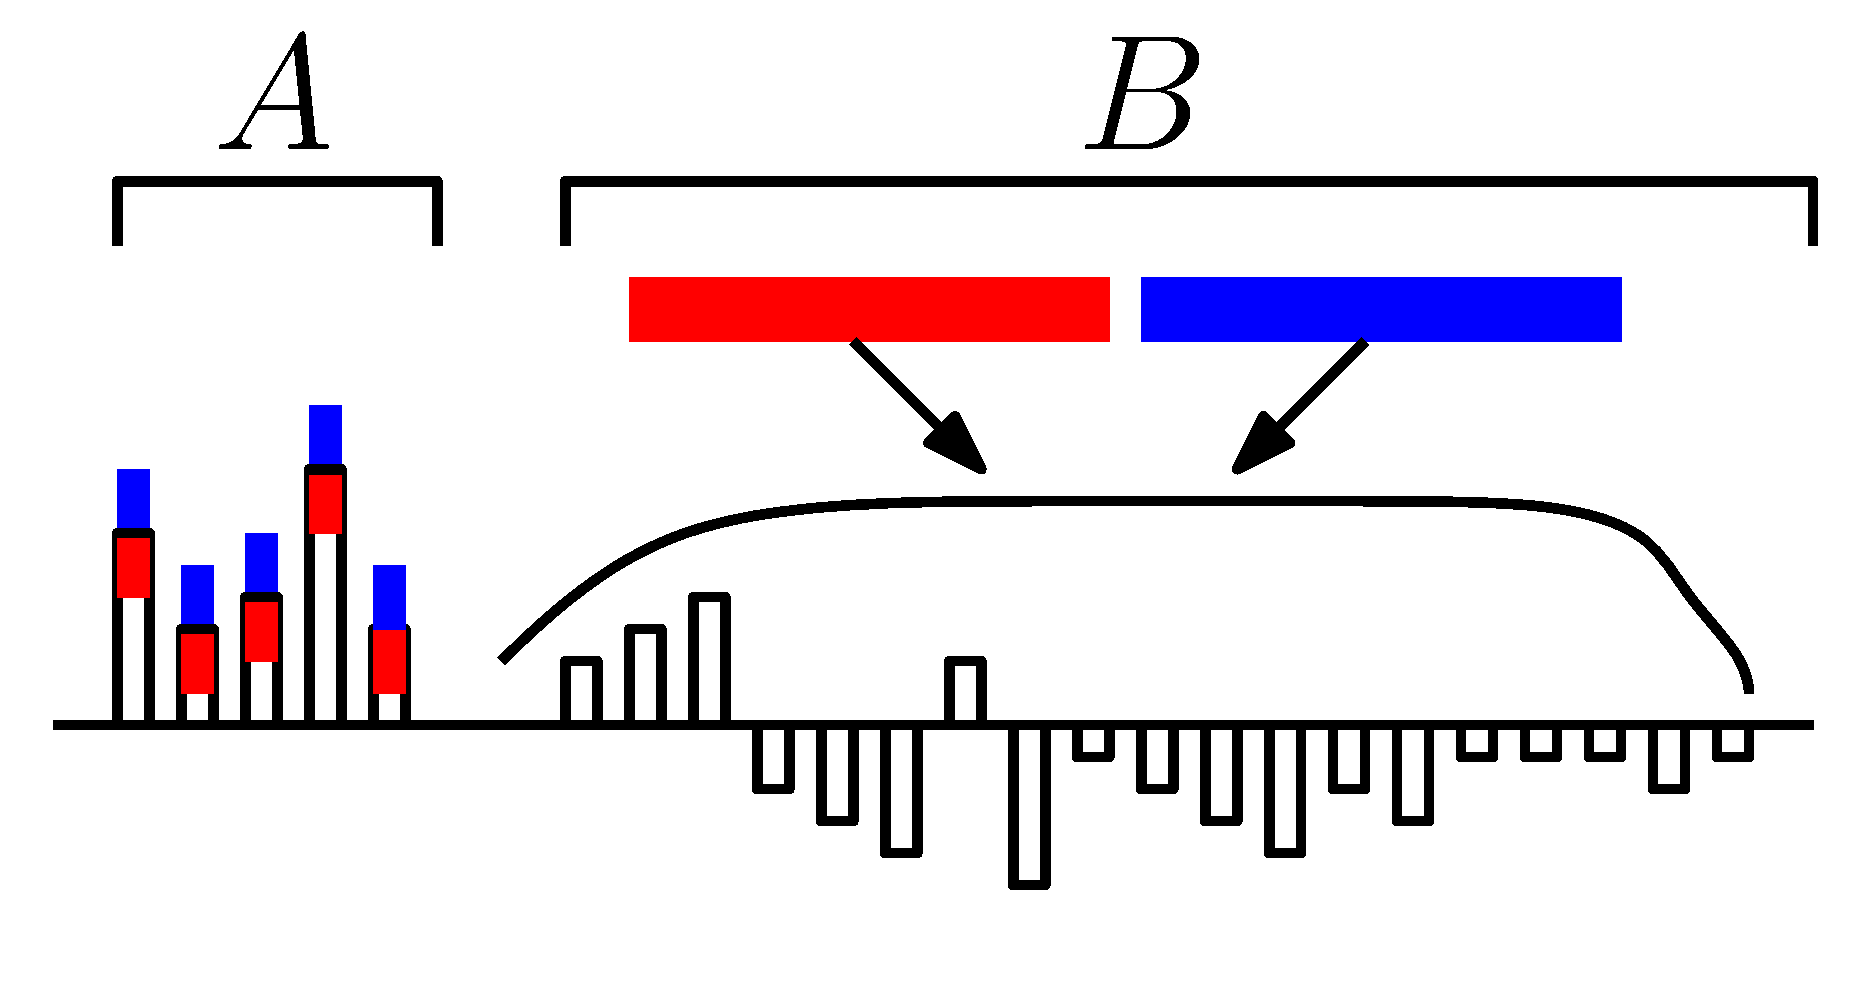
\includegraphics[width=\linewidth]{amppf/neglect0.eps}
    \onslide<3> 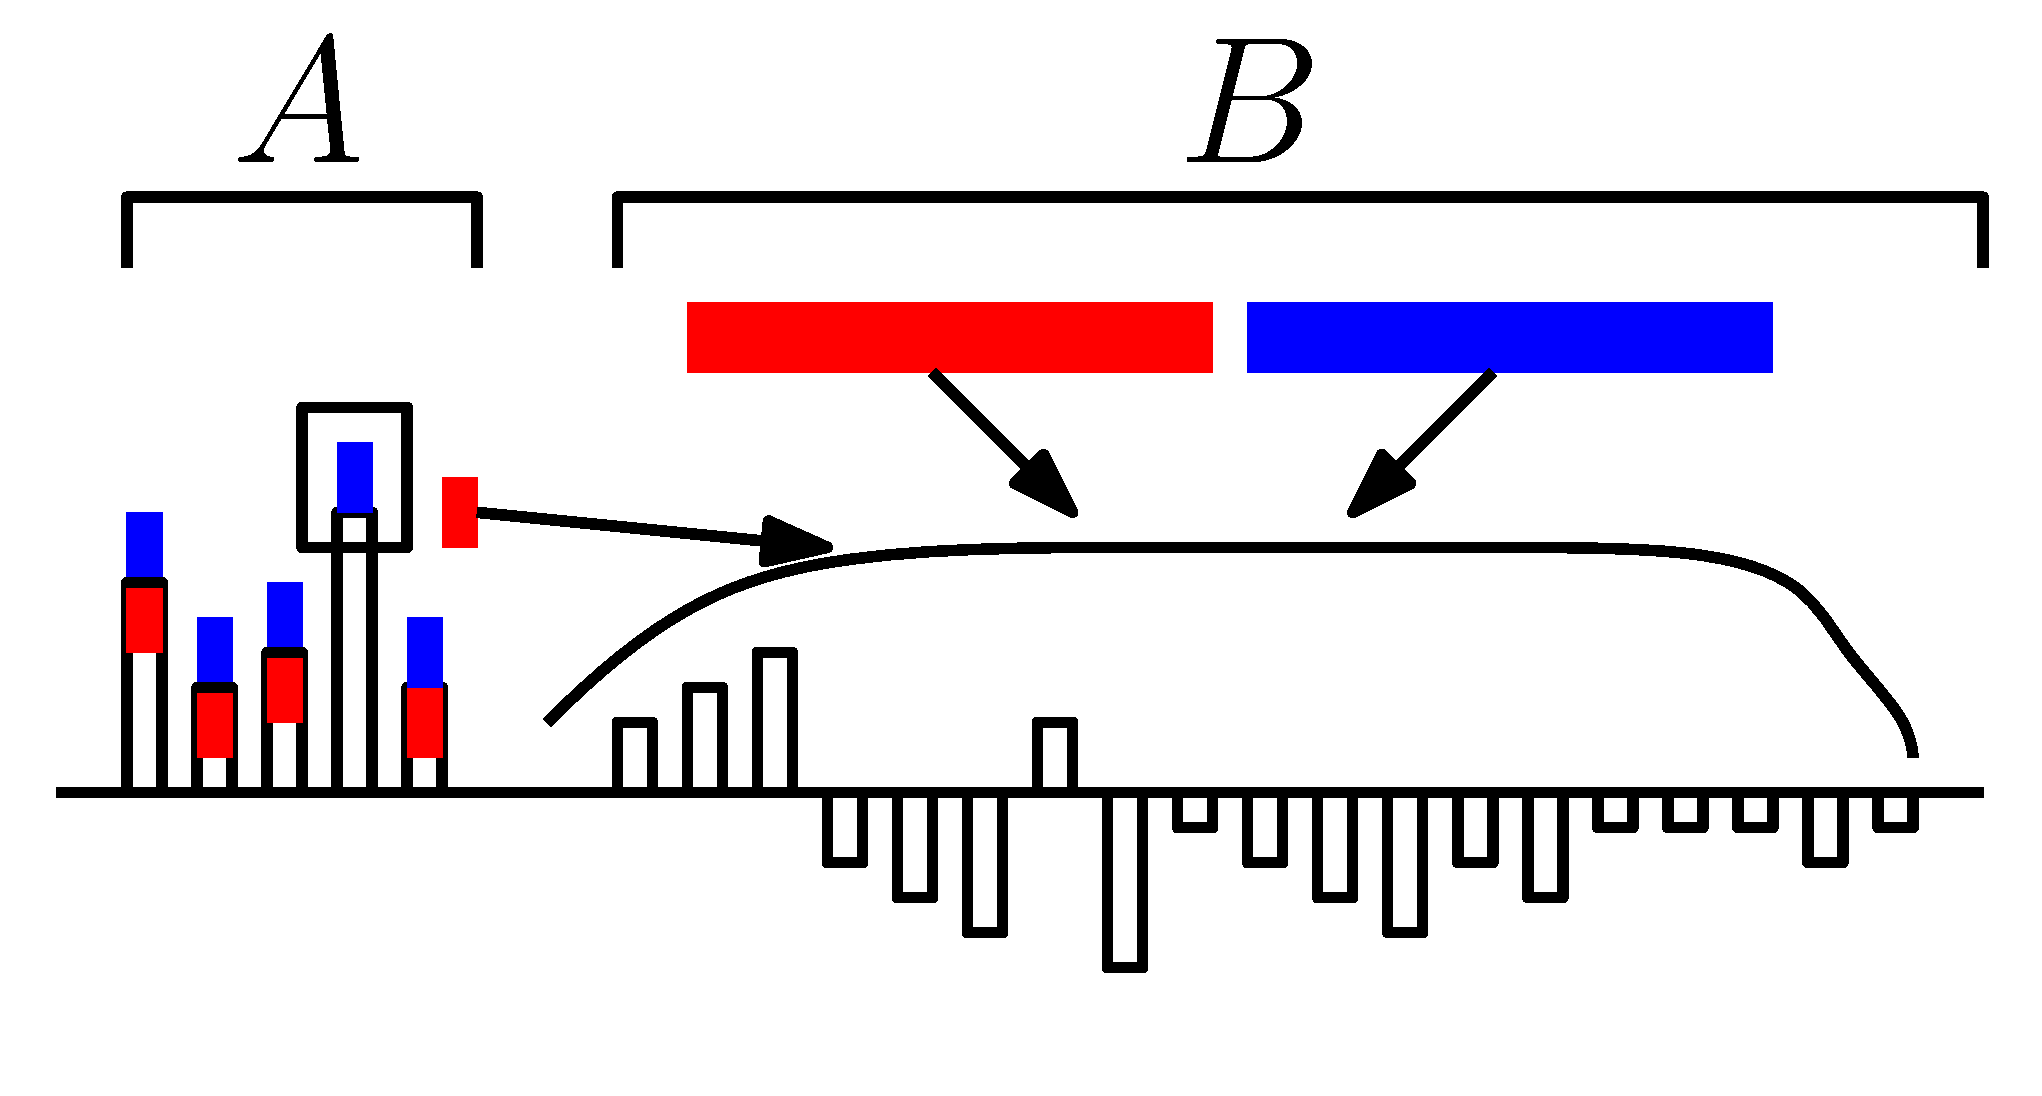
\includegraphics[width=\linewidth]{amppf/neglect1.eps}
    \onslide<4> 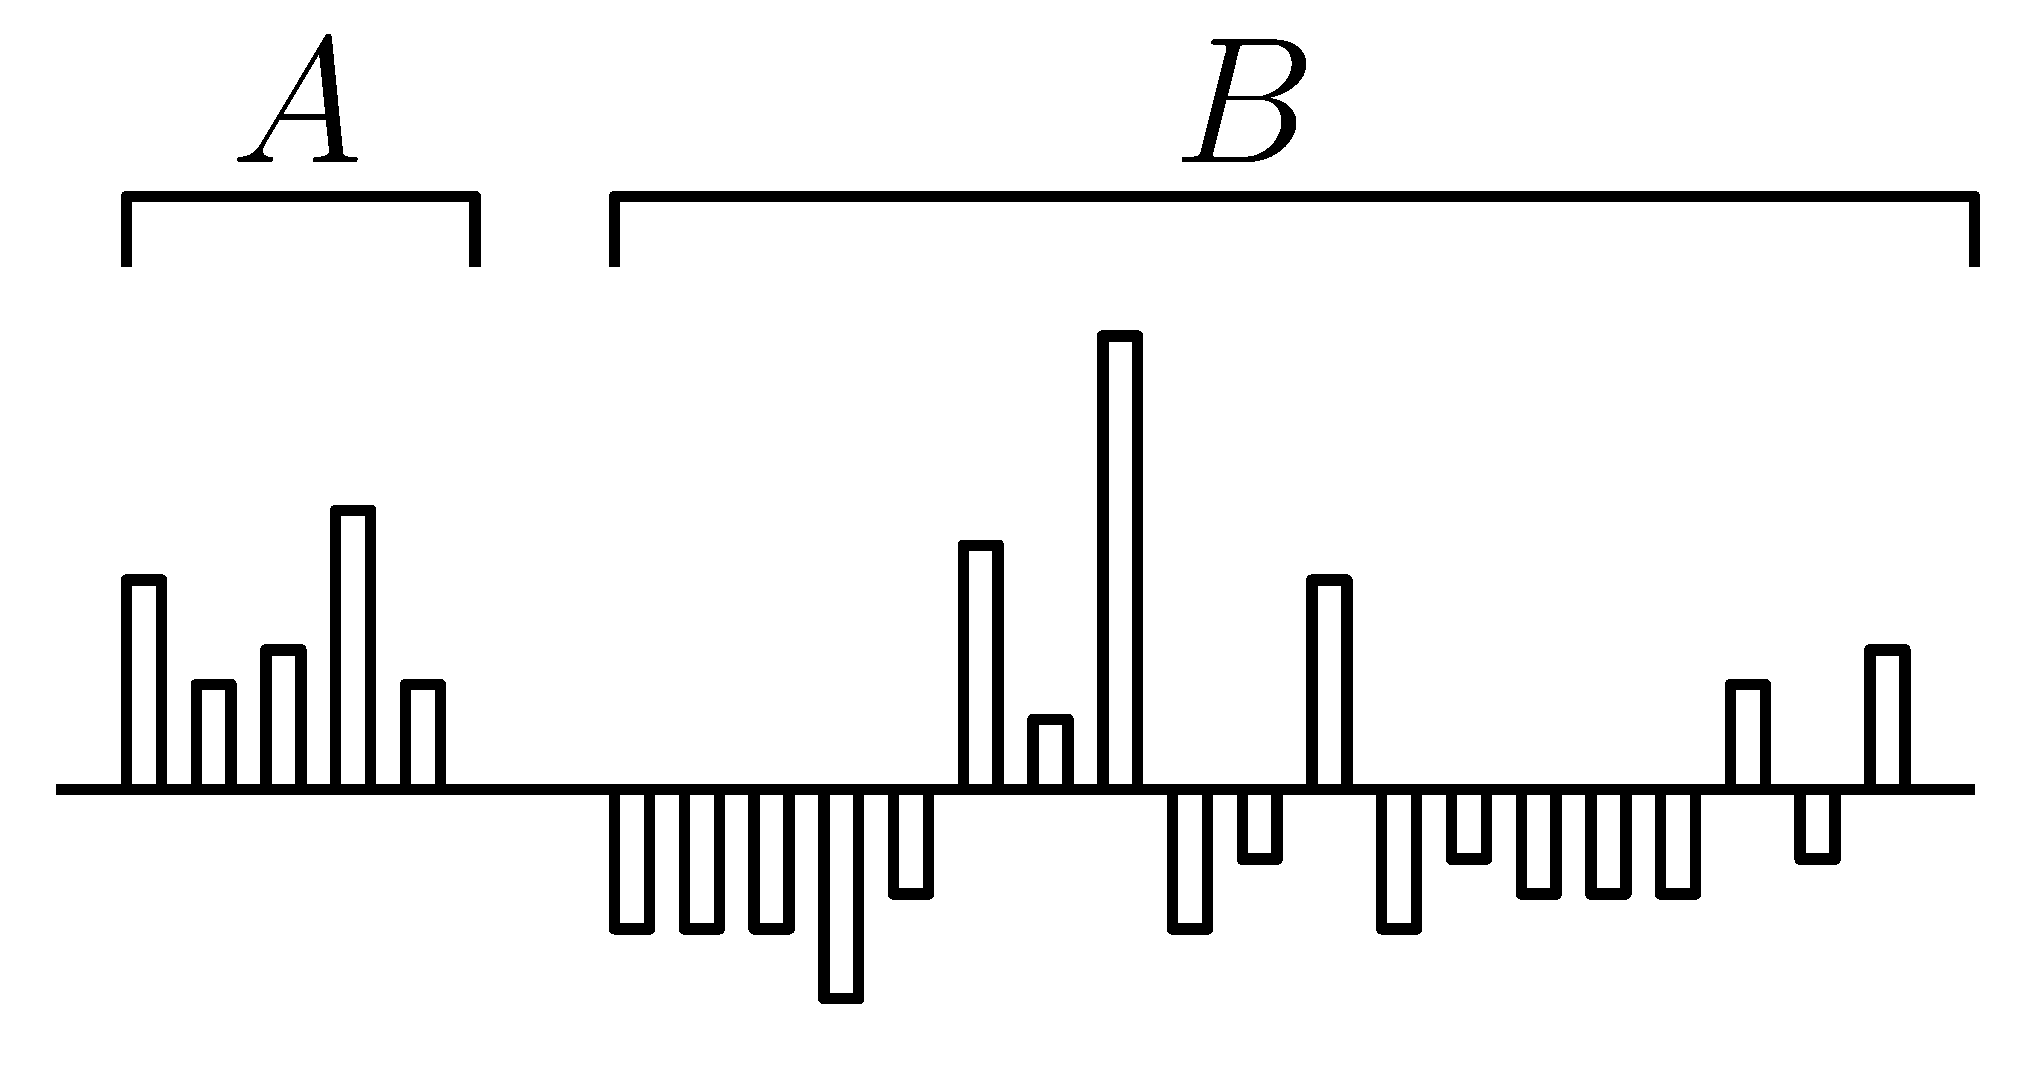
\includegraphics[width=\linewidth]{amppf/ani1.eps}
    \onslide<5> 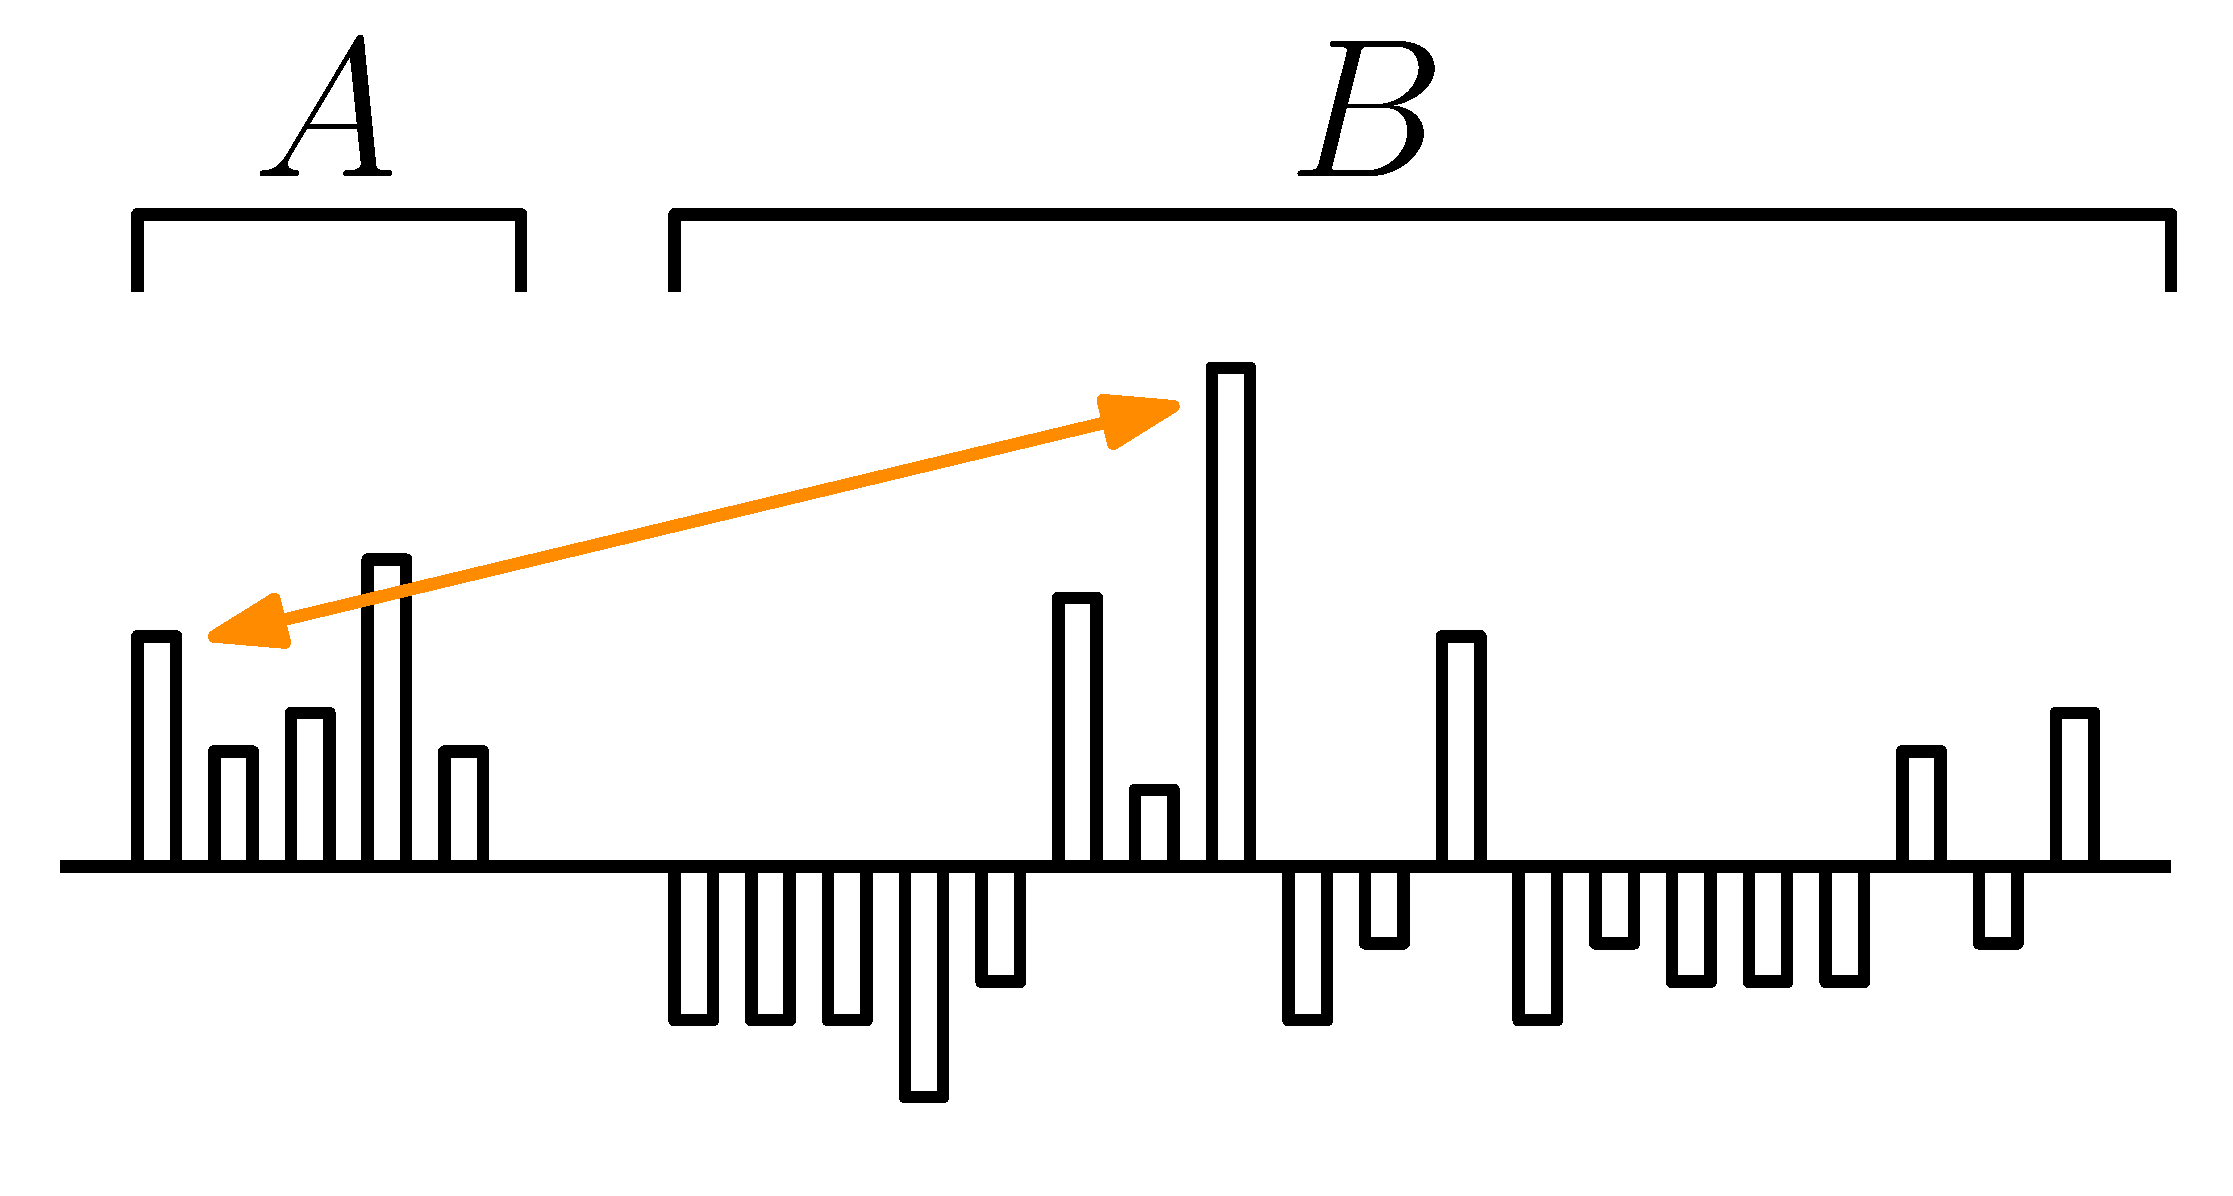
\includegraphics[width=\linewidth]{amppf/ani2.eps}
    \onslide<6> 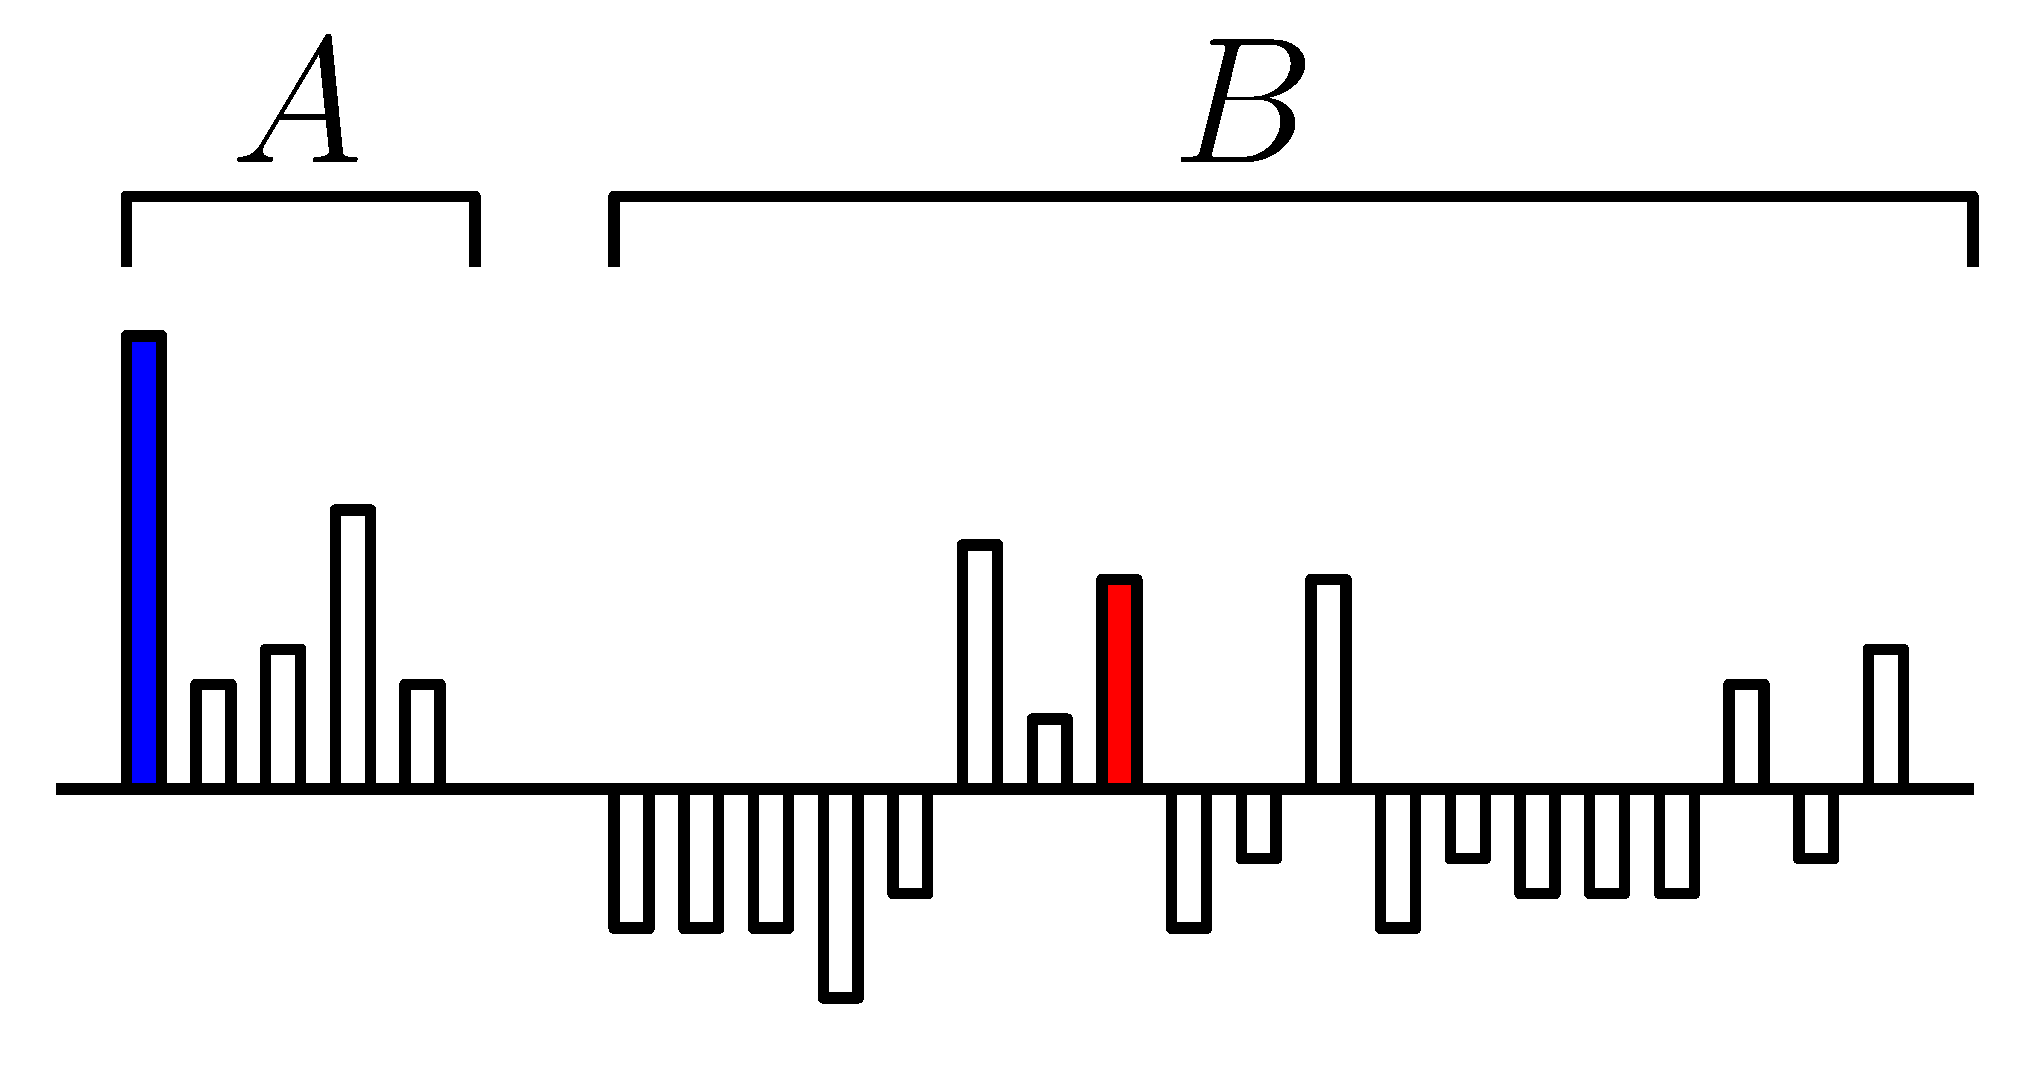
\includegraphics[width=\linewidth]{amppf/ani3.eps}
    \onslide<7> 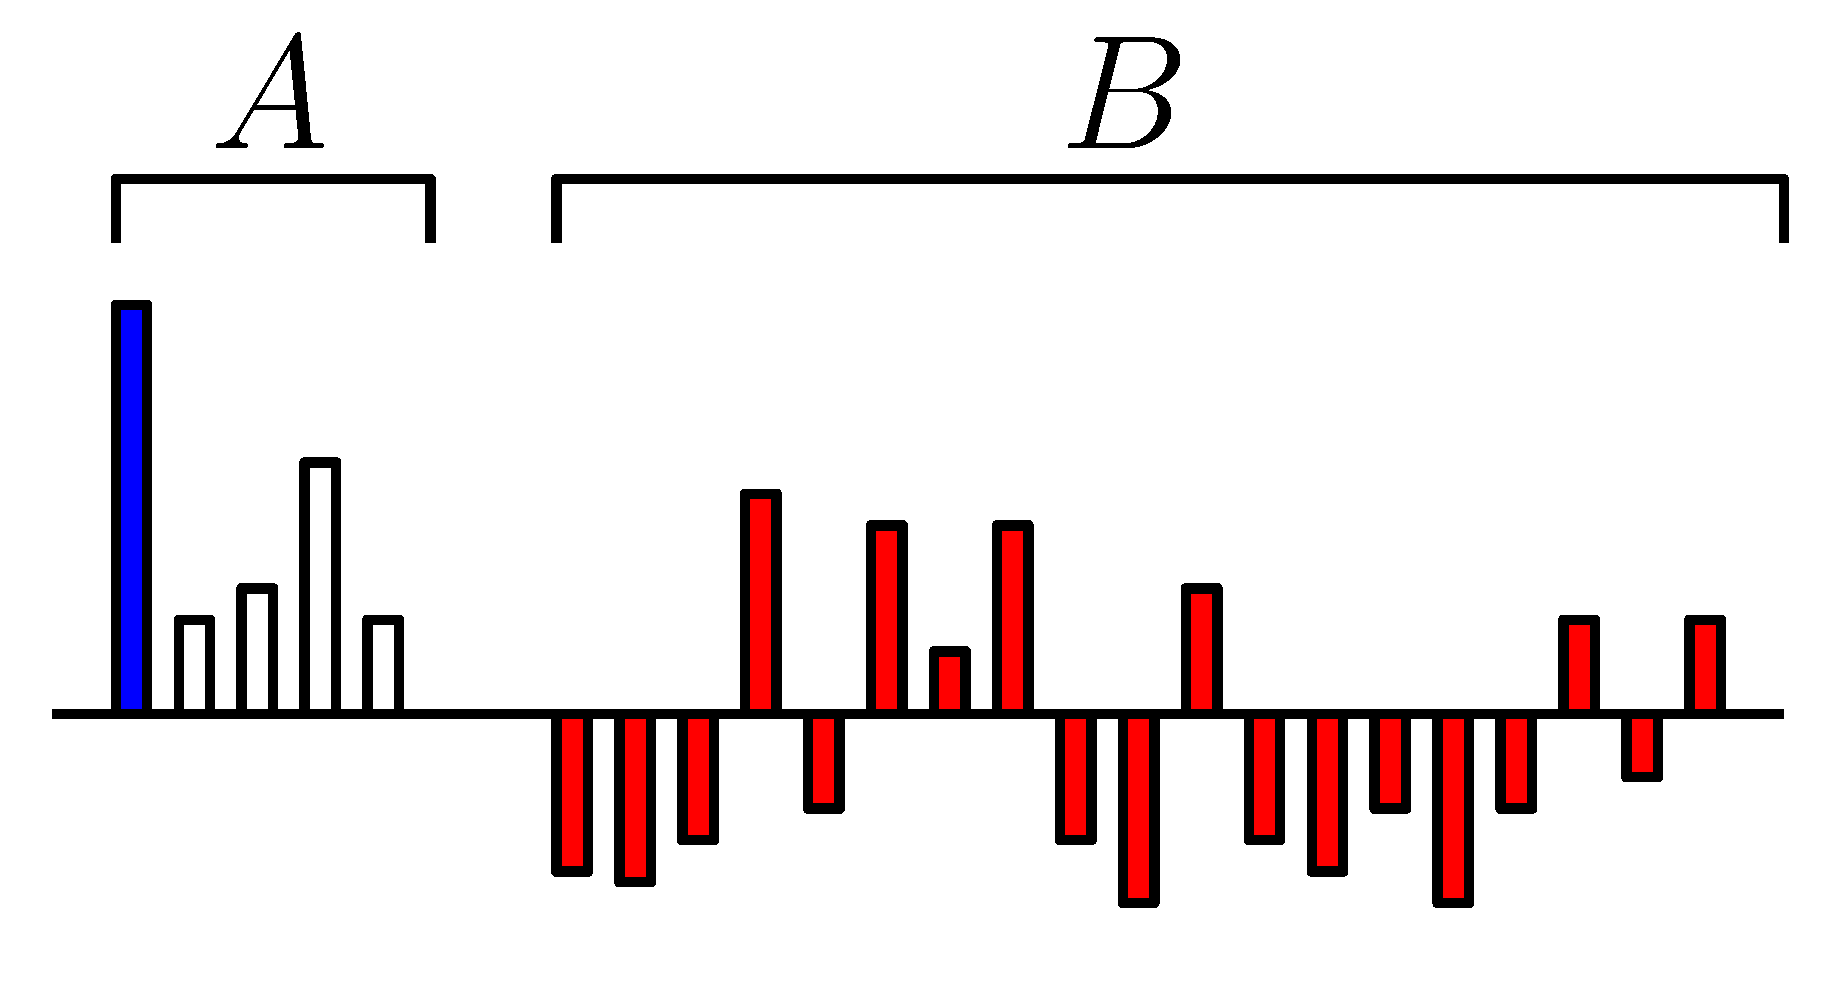
\includegraphics[width=\linewidth]{amppf/ani4.eps}
    \onslide<8> 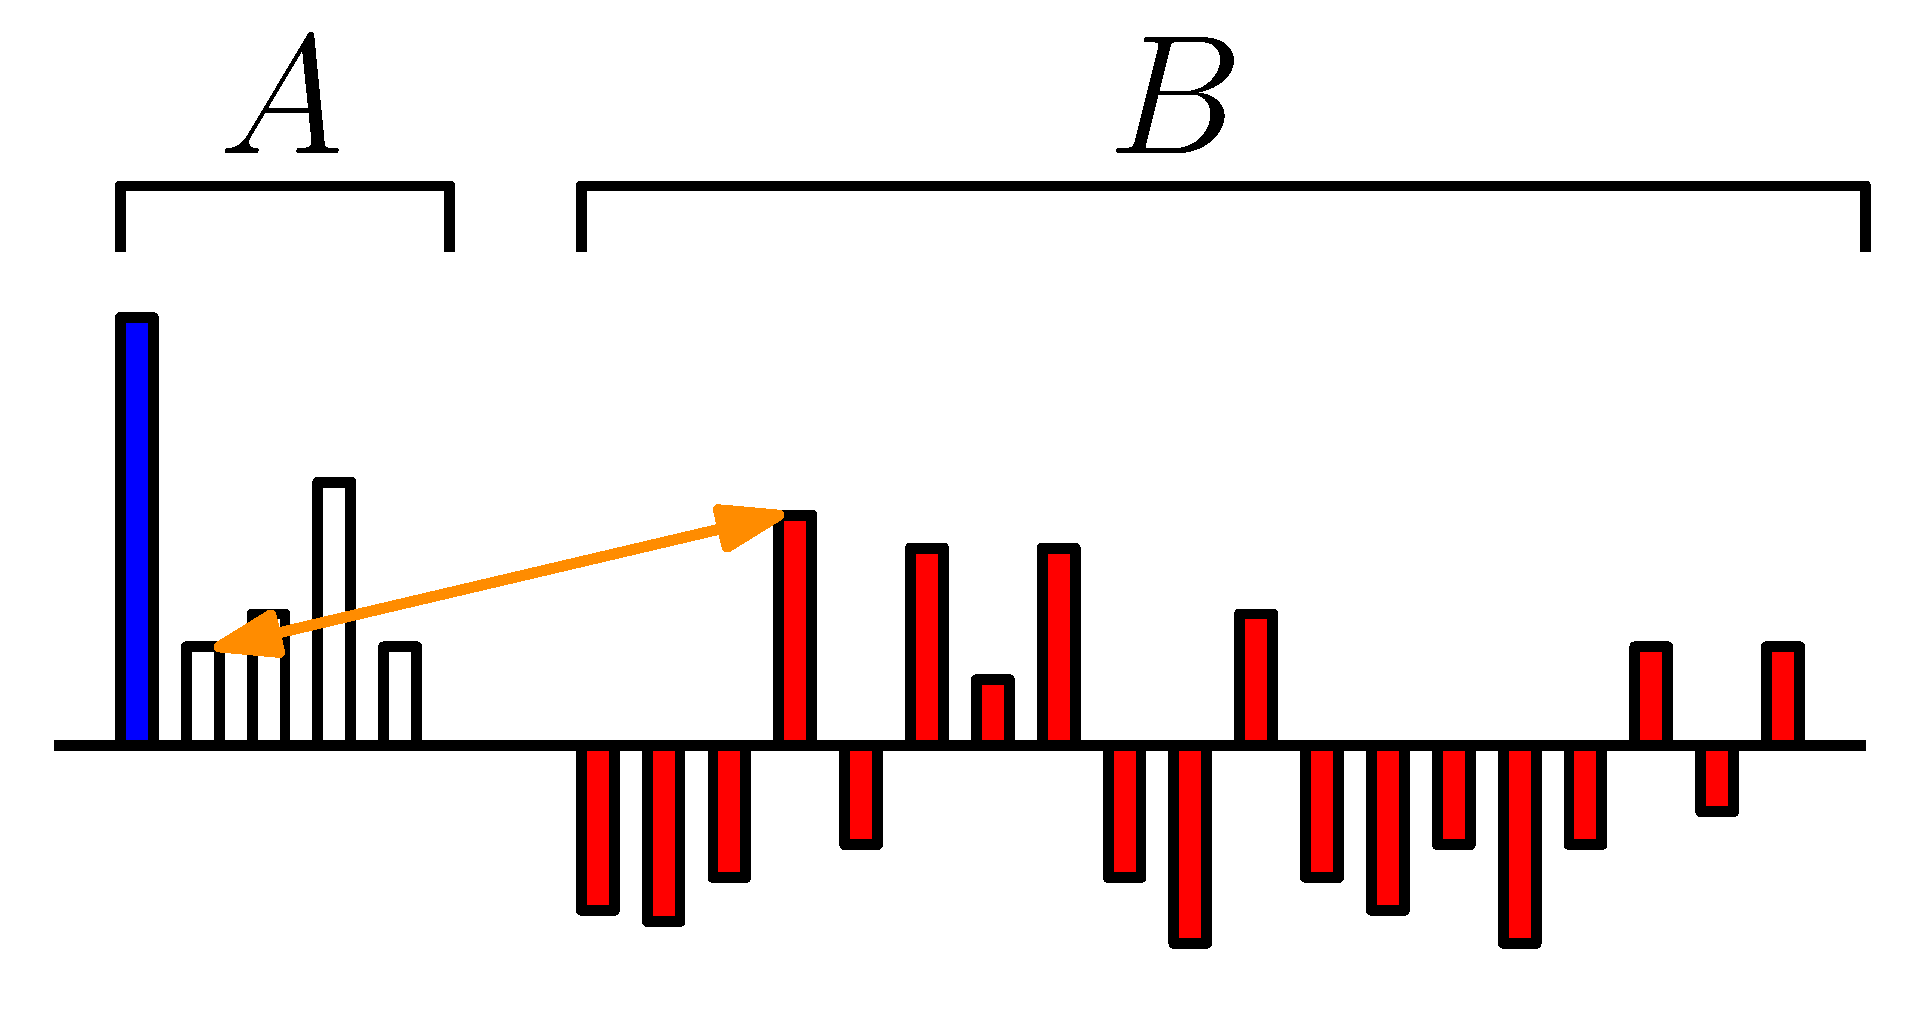
\includegraphics[width=\linewidth]{amppf/ani5.eps}
    \onslide<9> 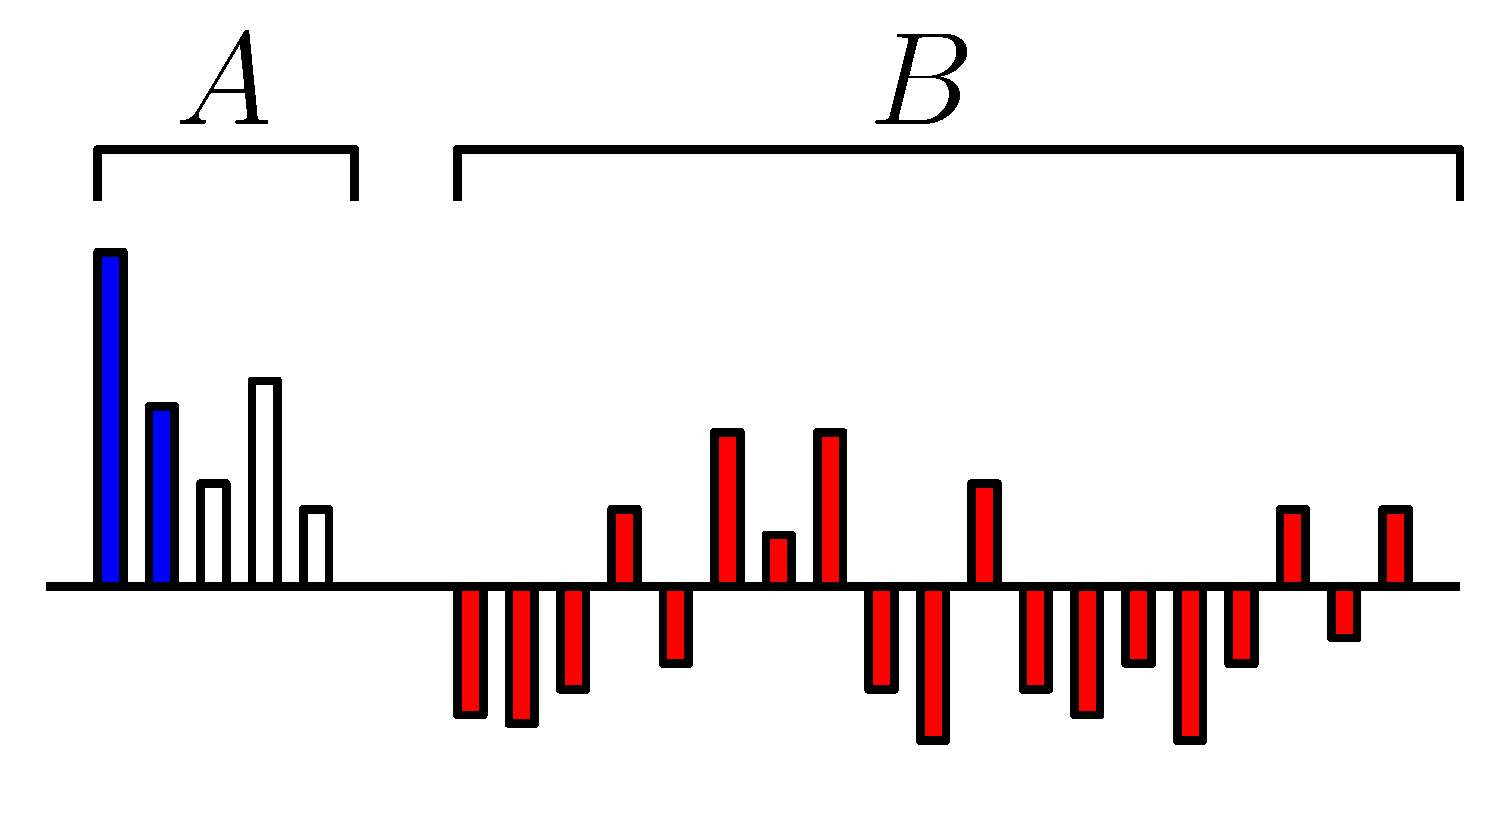
\includegraphics[width=\linewidth]{amppf/ani6.eps}
    \onslide<10> 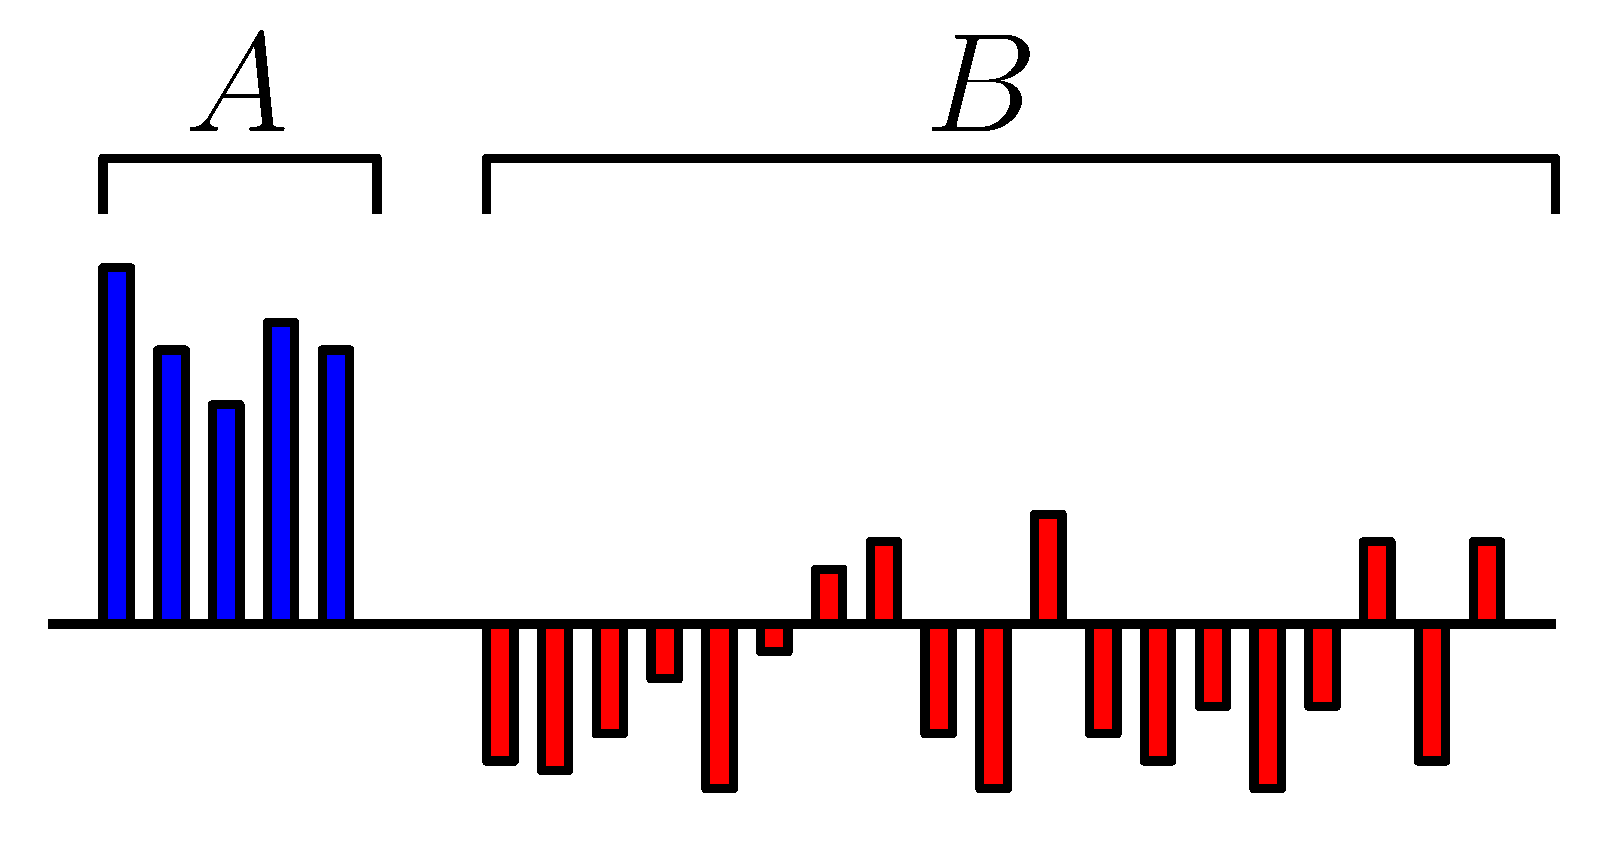
\includegraphics[width=\linewidth]{amppf/ani7.eps}
    \onslide<11> 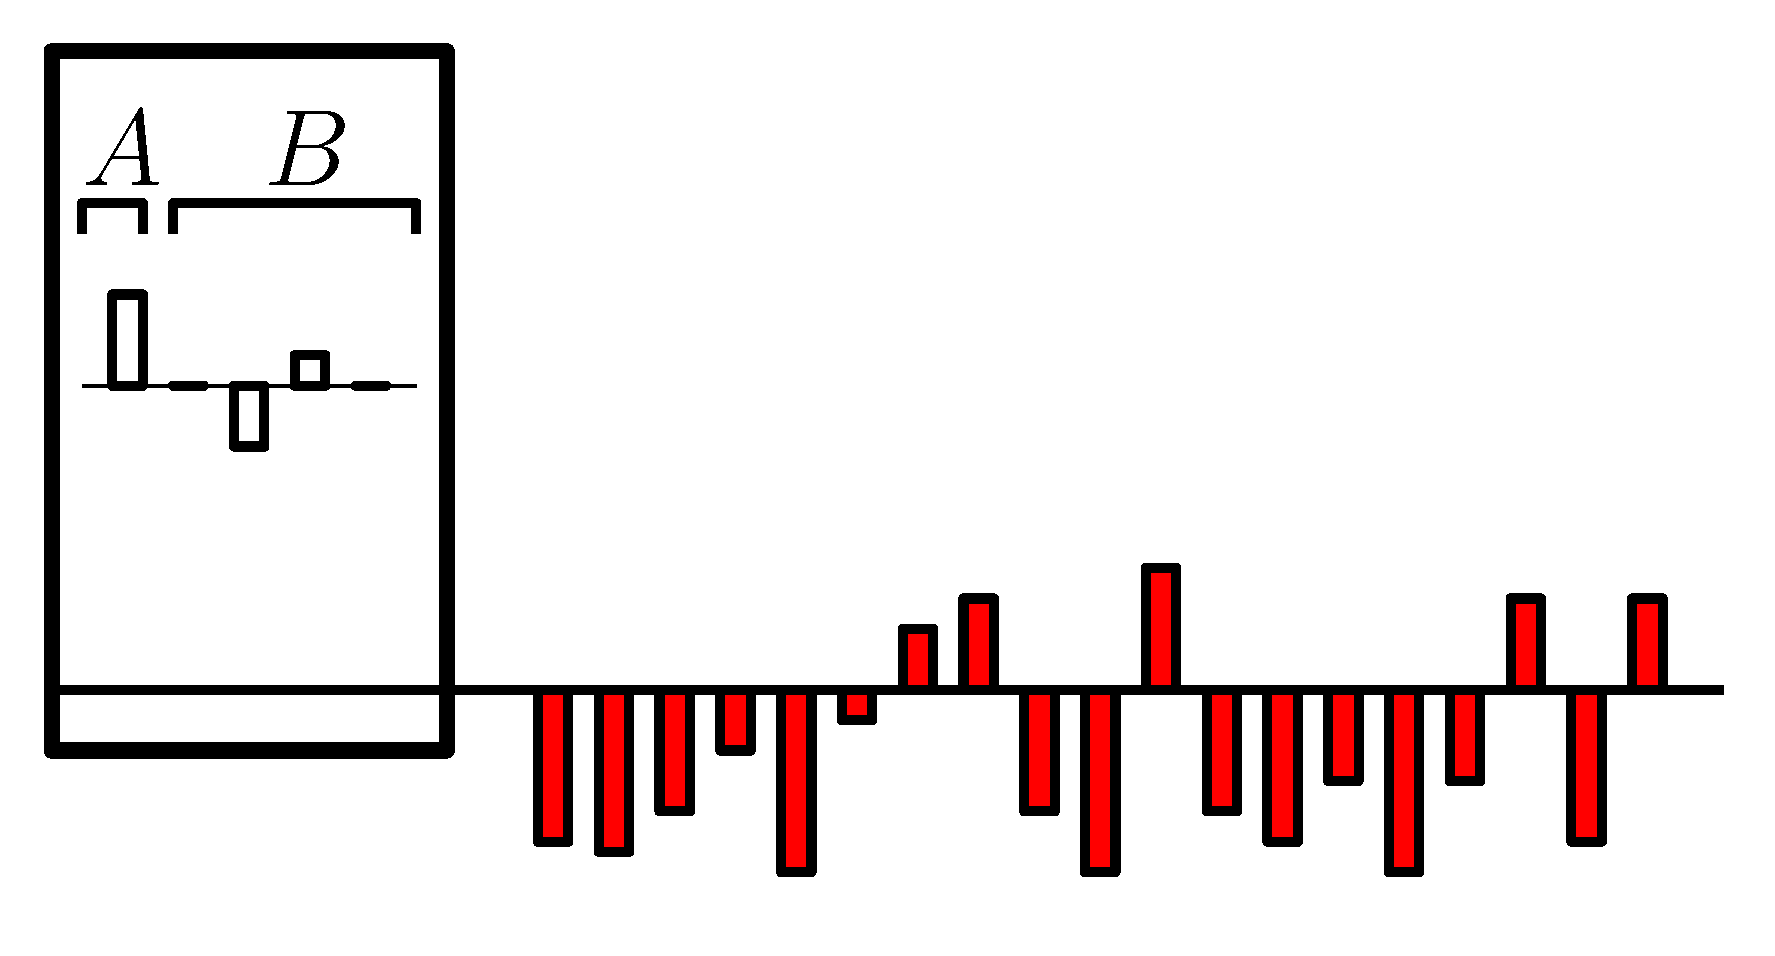
\includegraphics[width=\linewidth]{amppf/ani8.eps}
    \onslide<12> 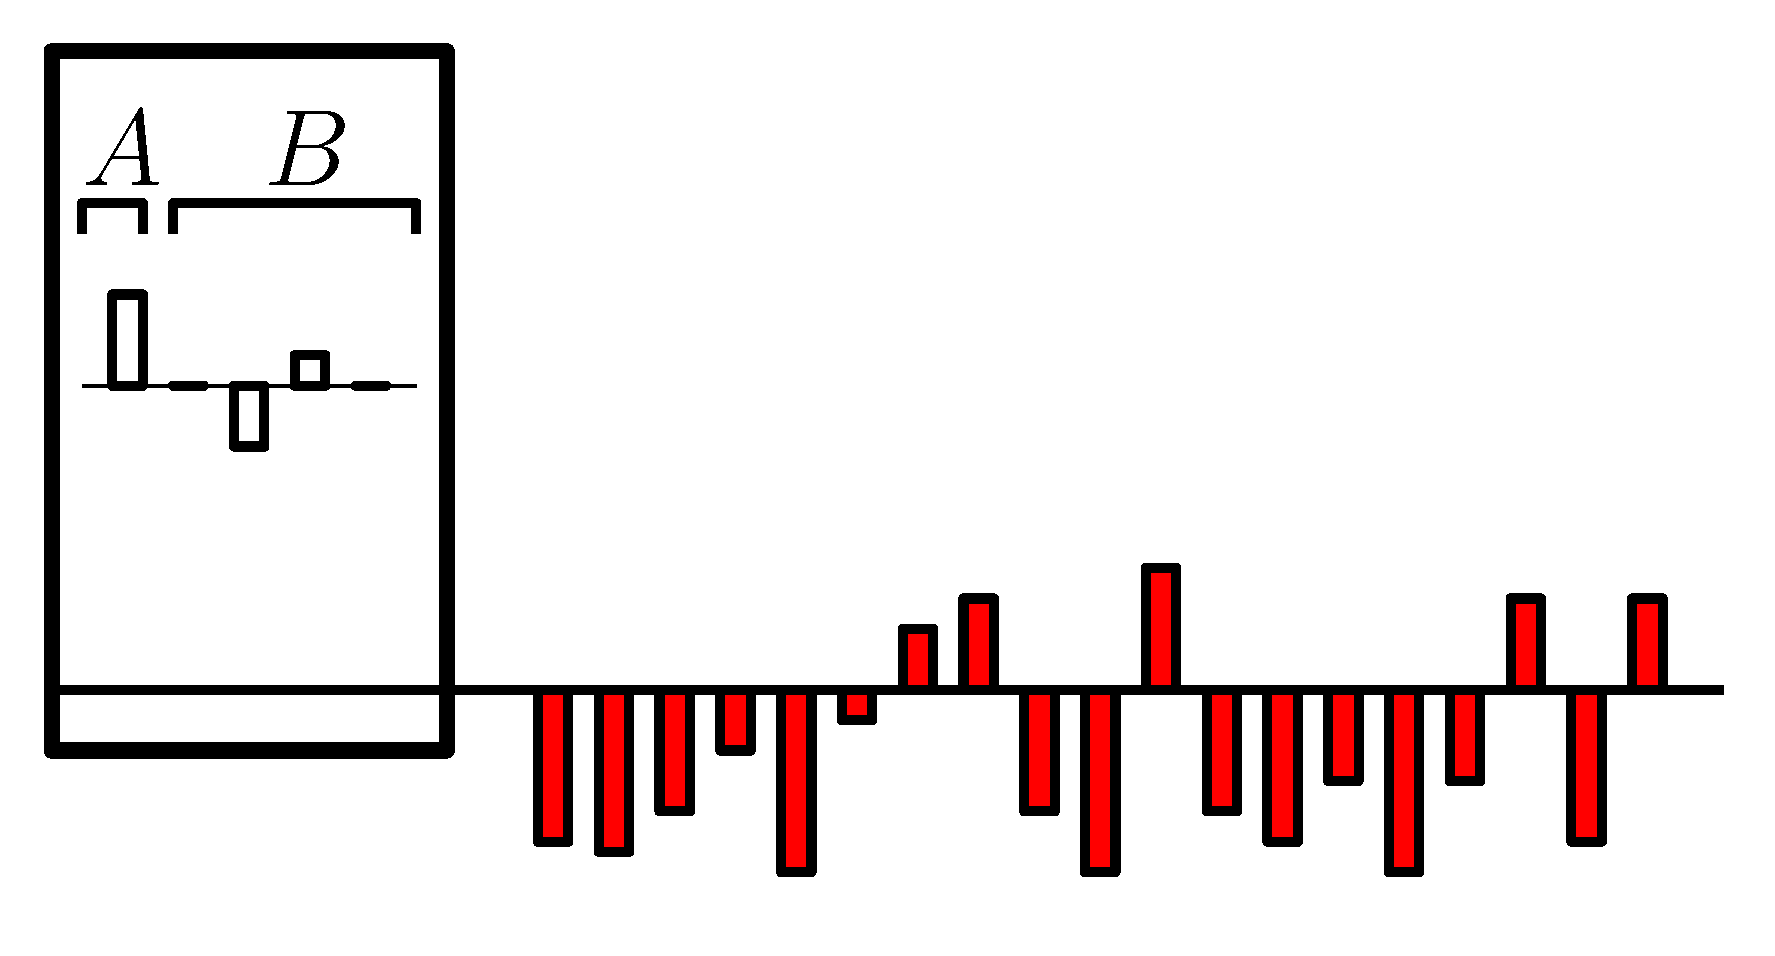
\includegraphics[width=\linewidth]{amppf/ani8.eps}
  \end{overprint}
  \begin{overprint}
    \onslide<1> Instantiate $A$ and $B$
    \onslide<2> Filling Strategy: Place $1$ fill in each cup in $A$, try to apply $f$ to $B$. 
    \onslide<3> If the emptier \defn{neglects} $A$
    then the average fill of $A$ rises! \\We
    repeat our strategy many times; if the emptier
    neglects $A$ too many times we get the desired
    backlog in $A$.
    \onslide<4> If emptier doesn't neglect $A$ filler can apply $f$ to $B$
    \onslide<5> Get a cup with high fill in $B$, swap it into $A$
    \onslide<6> Note: swaps increase average fill of $A$, decrease average fill of $B$.
    \onslide<7> Apply $f$ to $B$ again
    \onslide<8> Swap cup into $A$ again
    \onslide<9> Swap this cup into $A$.
    \onslide<10> Eventually average fill of $A$ is at least $(1-\delta)f(n(1-\delta)).$
    % After repeating this process for
    % each cup in $A$, the difference of the average
    % fills of $A$ and $B$ is at least $f(|B|)$; $A$
    % accounts for $|B|/n$ of this difference. Thus
    % average fill of $A$ has increased by at least
    % $(1-\delta)f((1-\delta)n)$
    \onslide<11> Recurse on $A$ for $L$ levels of recursion. \\Problem size shrinks by a factor of $\delta$ each time. 
    \onslide<12> $$f'(n) \ge (1-\delta)\sum_{\ell=0}^L f(n\delta^\ell(1-\delta))$$
  \end{overprint}
\end{frame}

\begin{frame}[t]{Adaptive Filler Lower Bound}
  Let $\epsilon > 0$ be any constant. There exists an appropriate $\delta=\Theta(1)$ such that by repeated amplification we get: 
  \begin{theorem}
    There is an adaptive filling strategy that achieves
    backlog $\Omega(n^{1-\epsilon})$  in running-time $2^{O(\log^2 n)}$.
  \end{theorem}
  \vspace{0.5cm}
  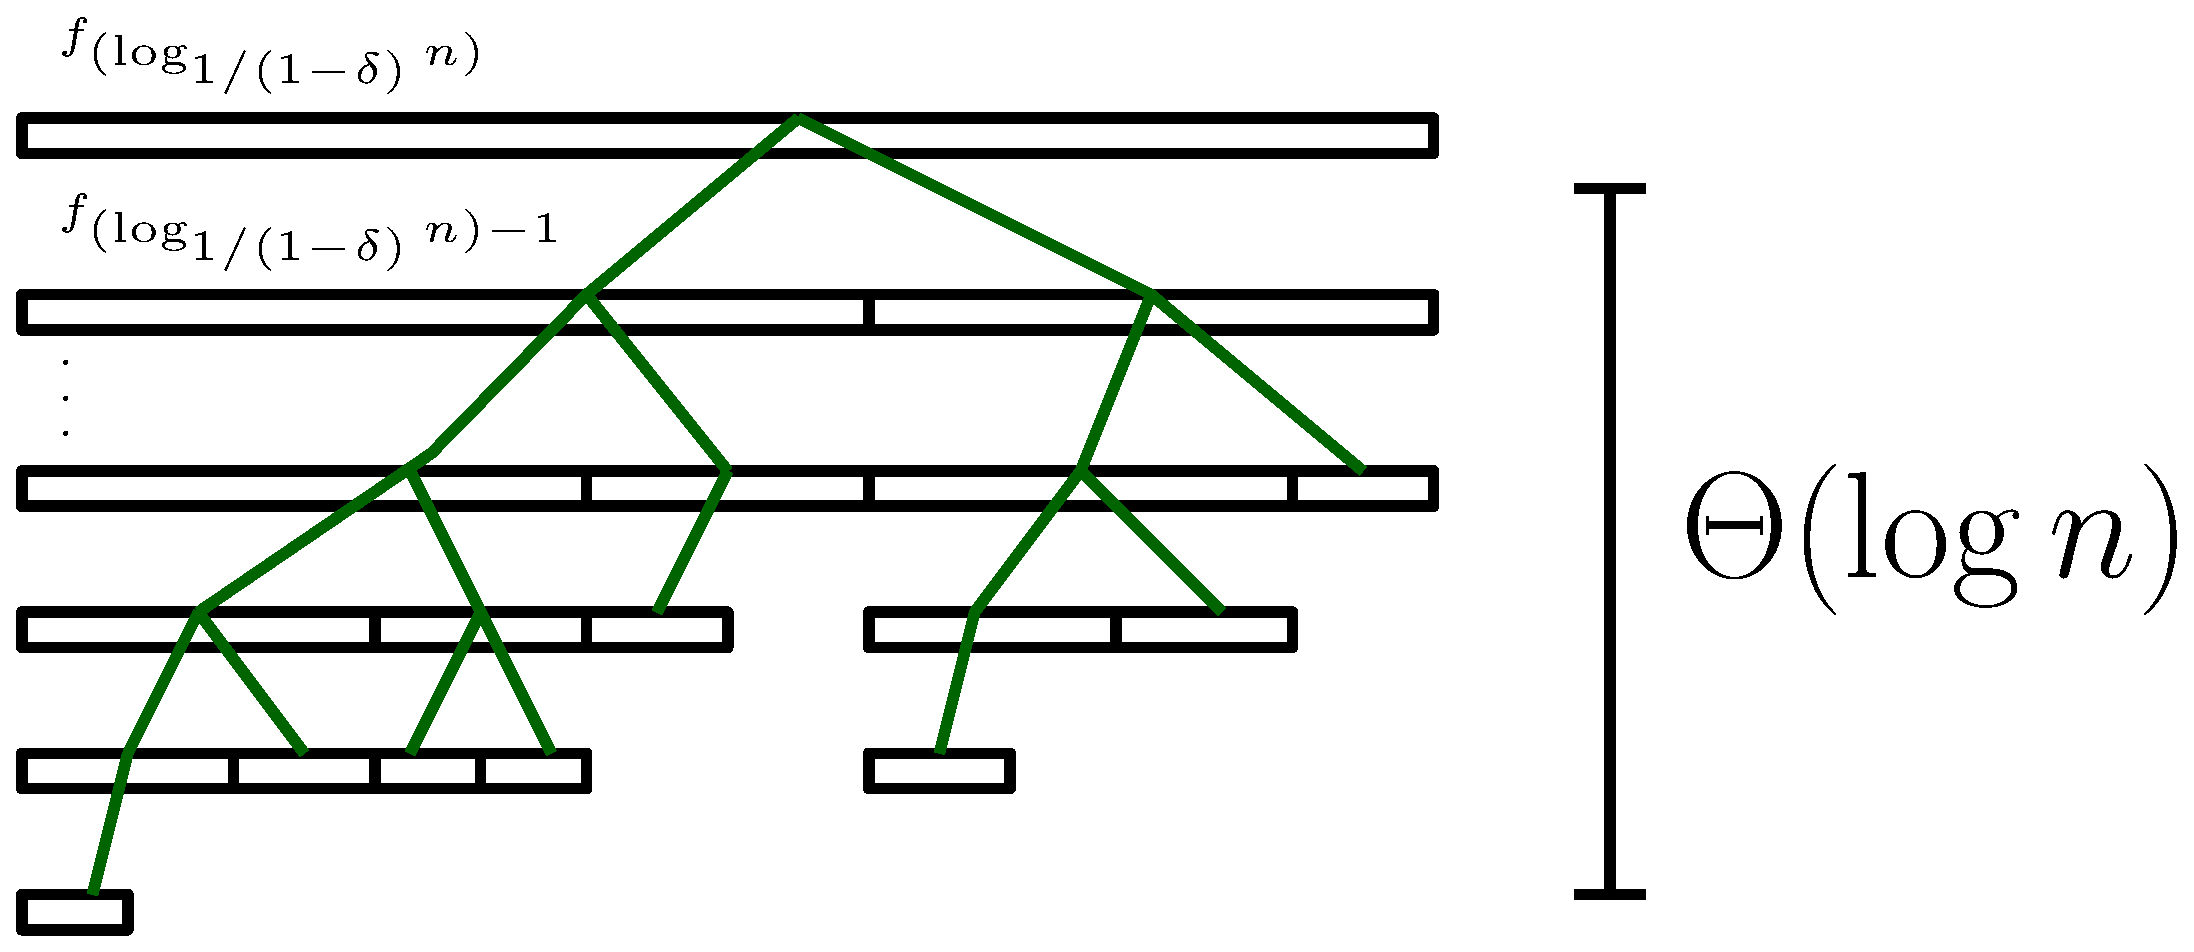
\includegraphics[width=0.7\linewidth]{amplificationImgs/quasipoly_cor.eps}
\end{frame}

\begin{frame}[t]{Adaptive Filler Lower Bound}
  Extremal strategy:\\
  By repeated amplification using $\delta=\Theta(1/n)$ we get: 
  \begin{theorem}
    There is an adaptive filling strategy that achieves backlog $\Omega(n)$ in running-time $O(n!)$.
  \end{theorem}
  \vspace{0.5cm}
  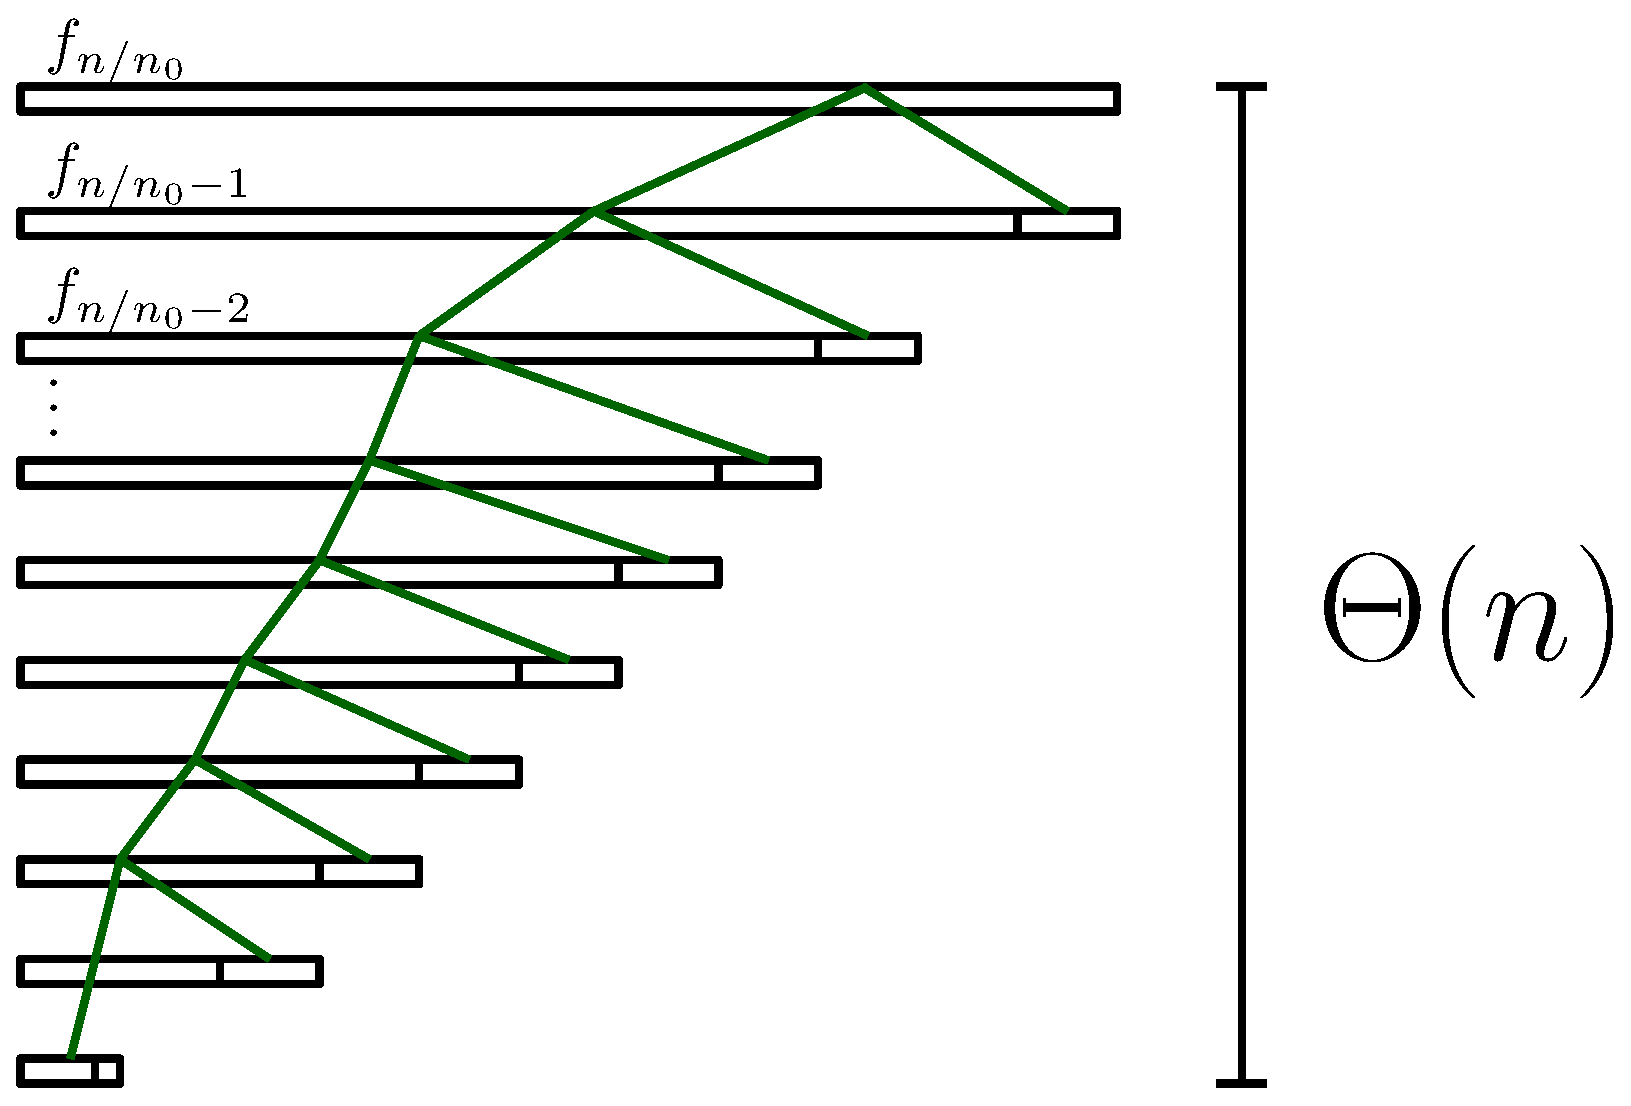
\includegraphics[width=0.45\linewidth]{amplificationImgs/expo_cor.eps}
\end{frame}

\begin{frame}[t]{Open Questions}
  \begin{itemize}
    \item Can we extend the oblivious lower bound construction to work with arbitrary emptiers?
    \item Are there shorter more simple constructions?
  \end{itemize}
\end{frame}

\begin{frame}[t]{Acknowledgements}
  \begin{itemize}
    \item My mentor William Kuszmaul
    \item MIT PRIMES
    \item My Parents
 \end{itemize} 
\end{frame}

\begin{frame}[c]{}
\begin{center}
\Huge Question Slides
\end{center}
\end{frame}

\begin{frame}[t]{What is the Cup Game?}
  \begin{definition}
  \defn{$p$-processor cup-game} on $n$ cups: \\
  multi-round game. every round:
  \begin{itemize}
    \item \defn{filler} adds water
    \item \defn{emptier} removes water
  \end{itemize}
  \end{definition}

  \vspace{0.4cm}
  Note: \\
  Emptier must allocate resources discretely\\
  Filler can allocate resources continuously
\end{frame}

\begin{frame}[t]{Single-Processor Lower Bound}
  \textbf{Filling strategy}: \\Distribute water equally amongst cups not yet emptied from.
  \vspace{0.3cm}
  \begin{overprint}
    \onslide<1>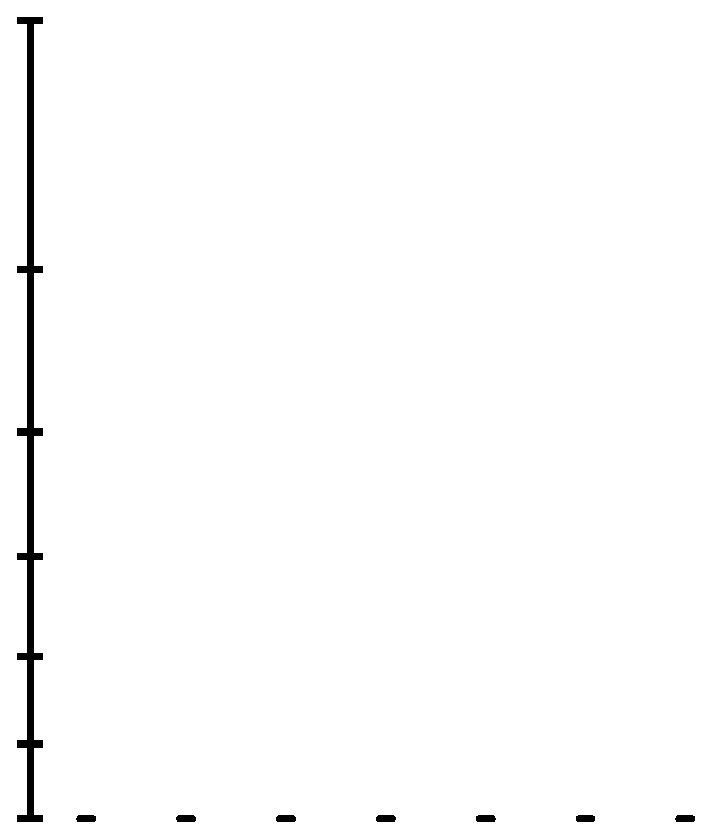
\includegraphics[width=0.5\linewidth]{singleProcessorLowerBound/round_0_1.eps}
    \onslide<2>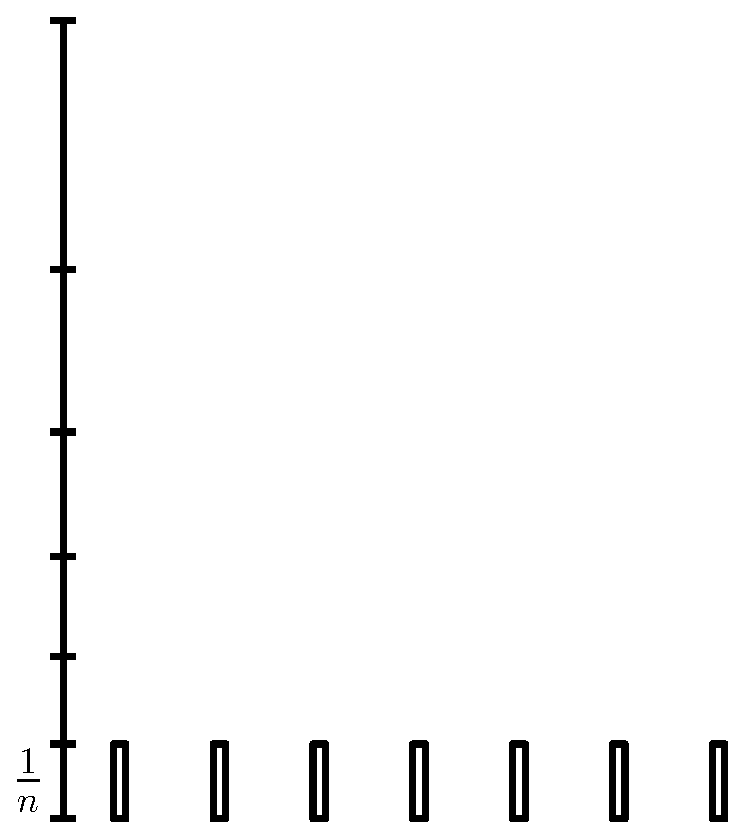
\includegraphics[width=0.5\linewidth]{singleProcessorLowerBound/round_1_0.eps}
    \onslide<3>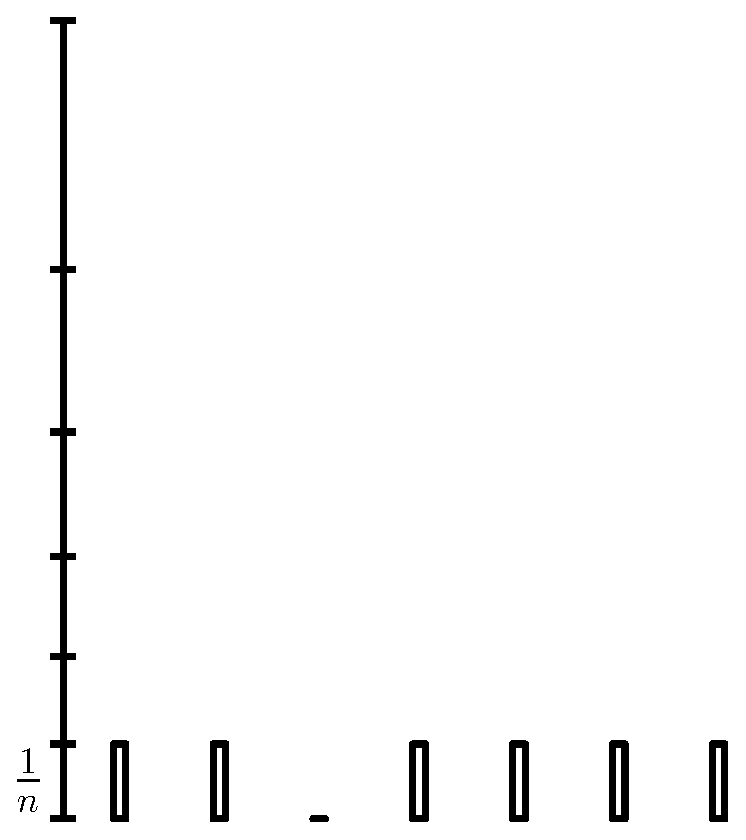
\includegraphics[width=0.5\linewidth]{singleProcessorLowerBound/round_1_1.eps}
    \onslide<4>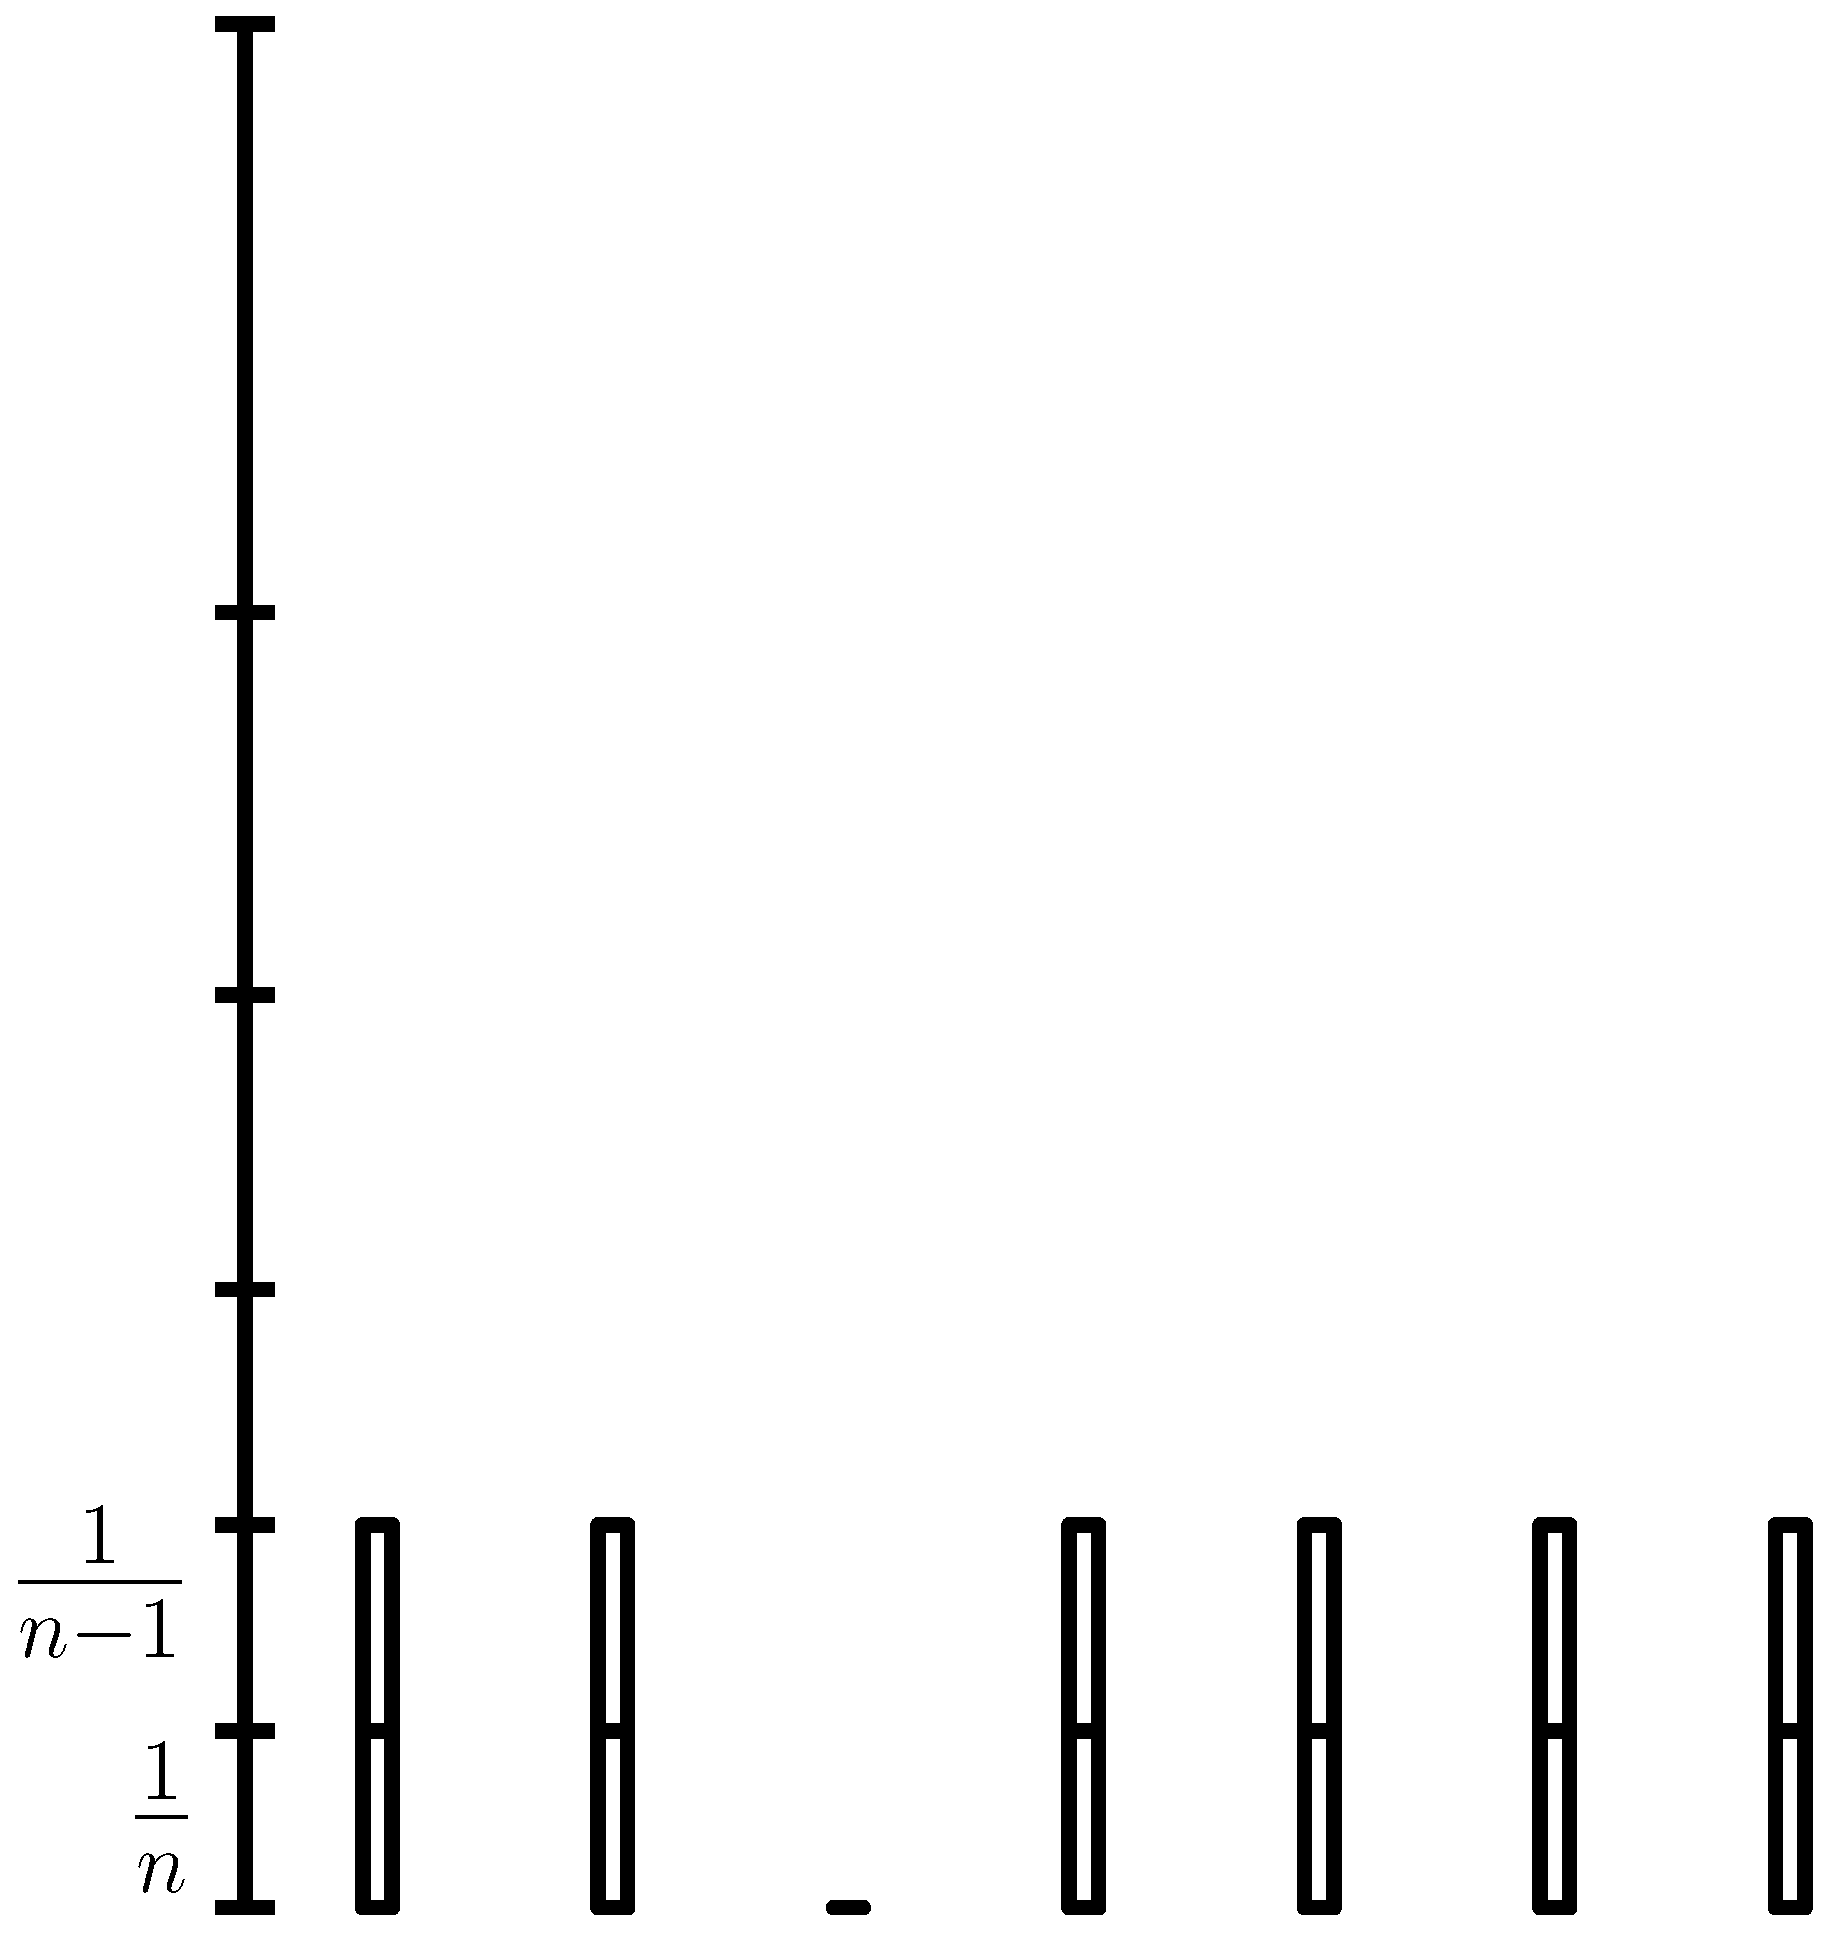
\includegraphics[width=0.5\linewidth]{singleProcessorLowerBound/round_2_0.eps}
    \onslide<5>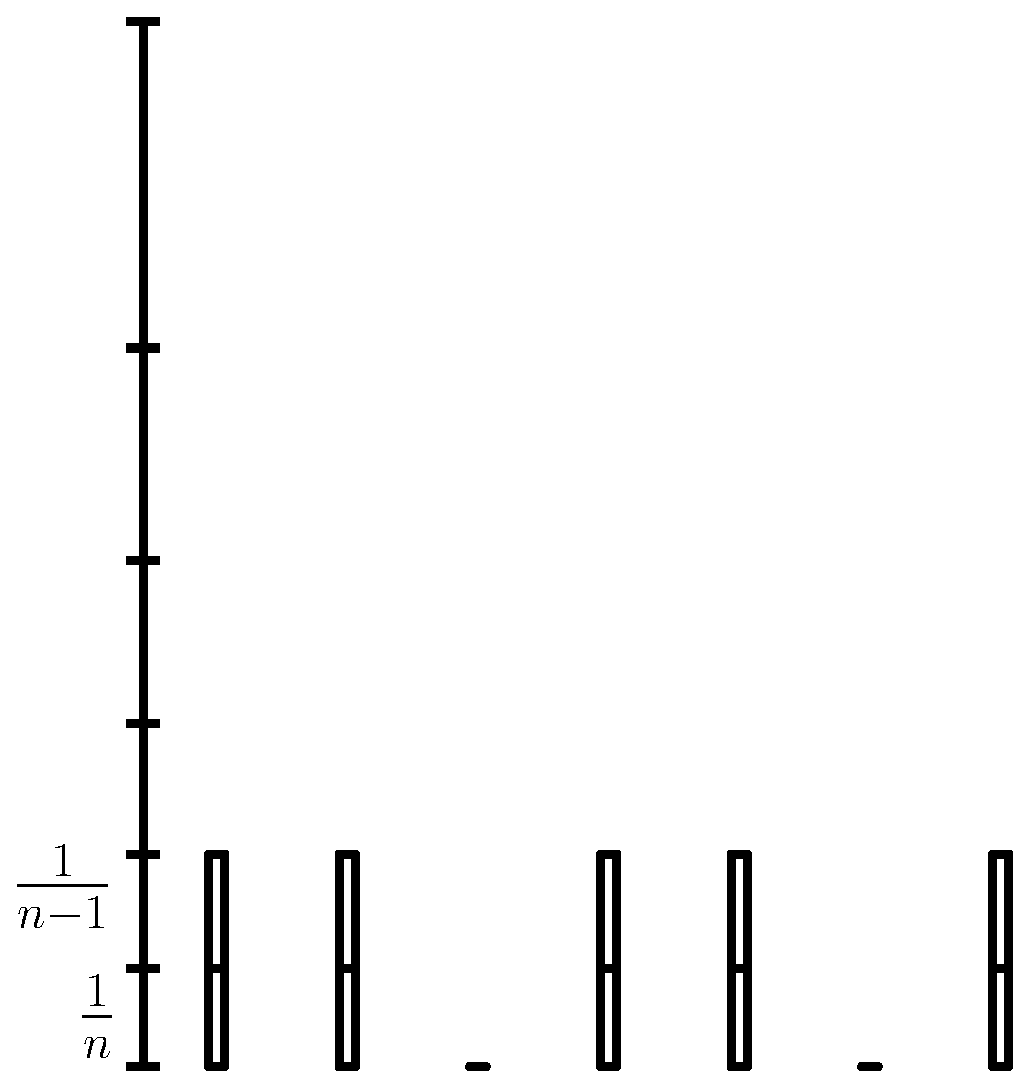
\includegraphics[width=0.5\linewidth]{singleProcessorLowerBound/round_2_1.eps}
    \onslide<6>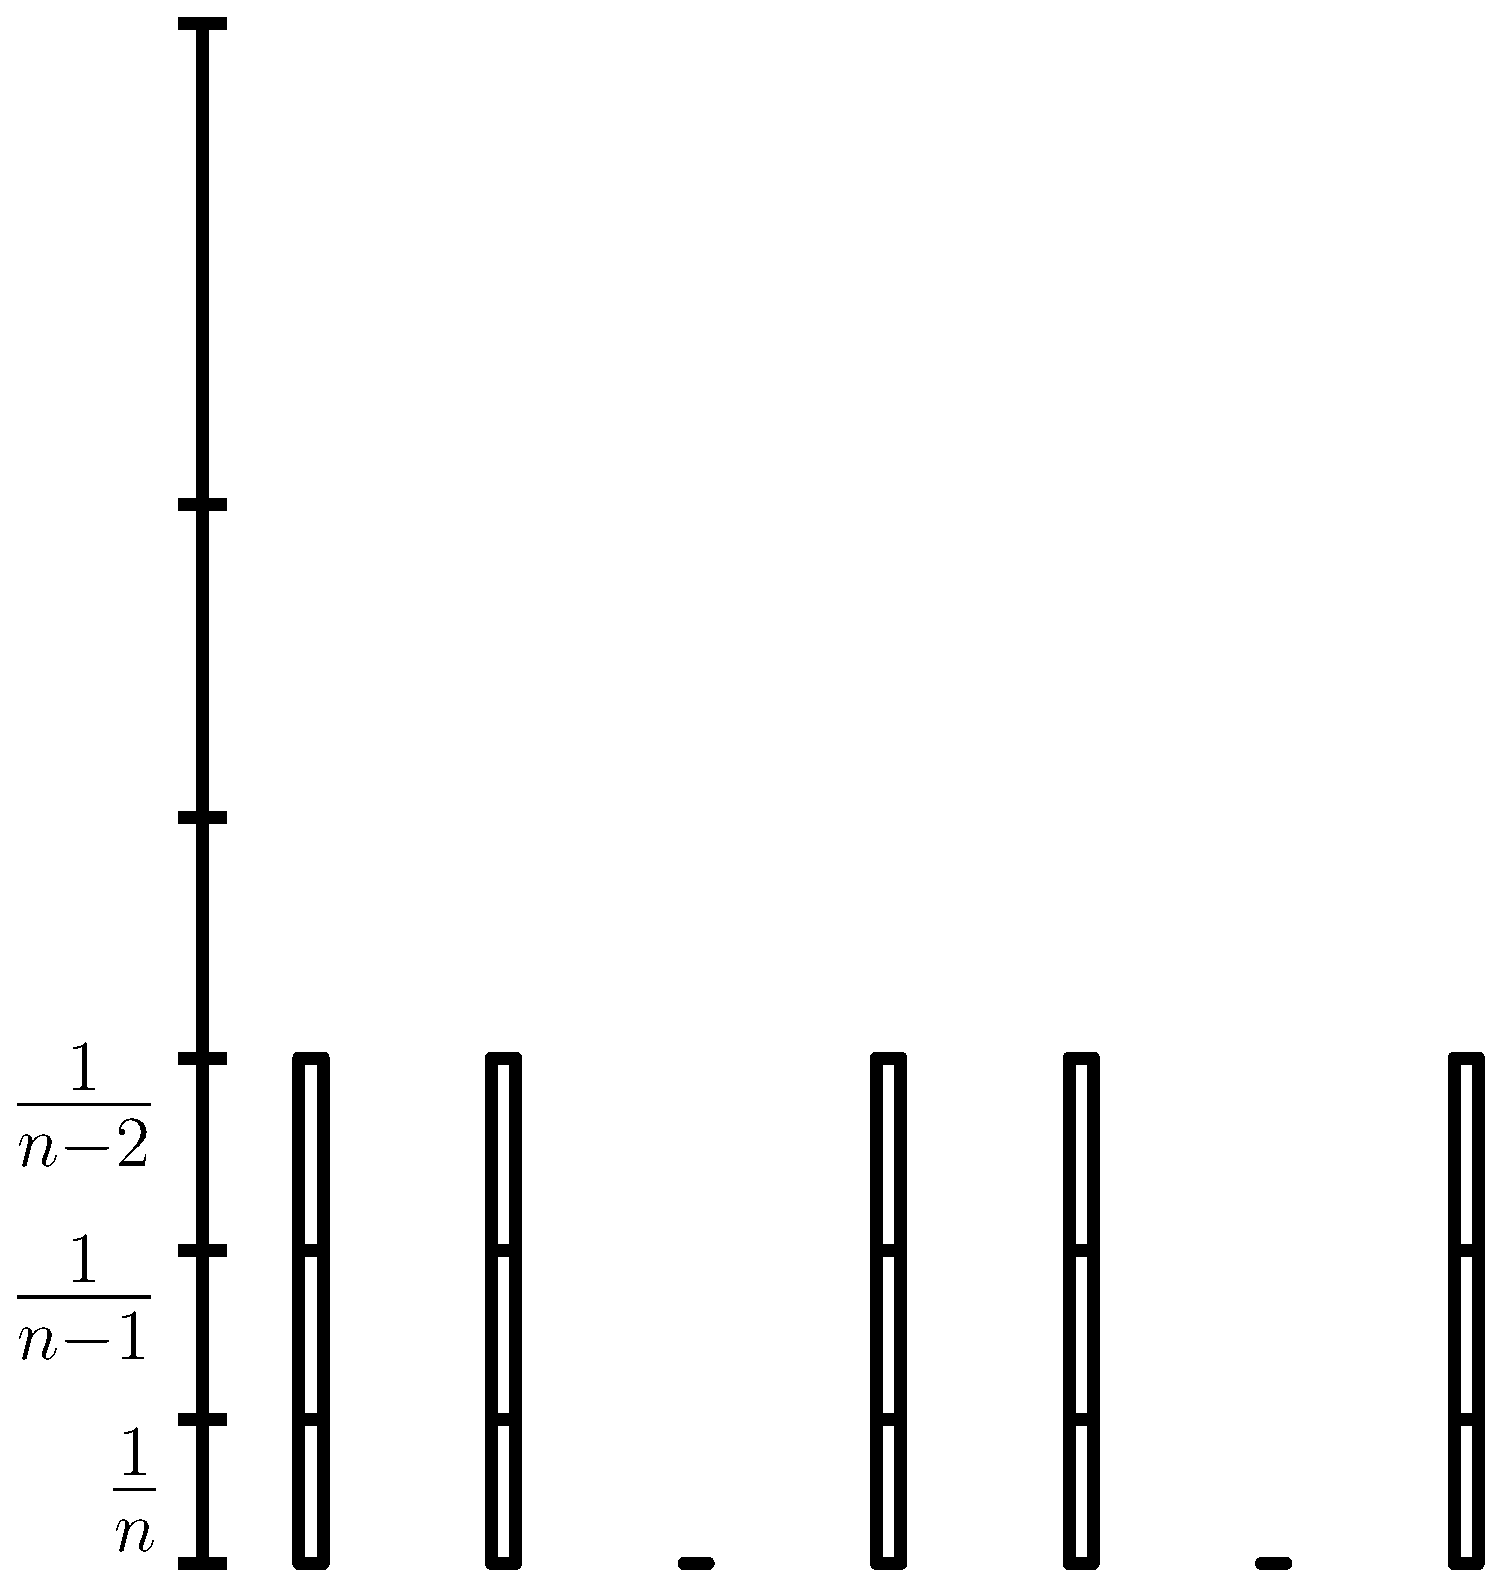
\includegraphics[width=0.5\linewidth]{singleProcessorLowerBound/round_3_0.eps}
    \onslide<7>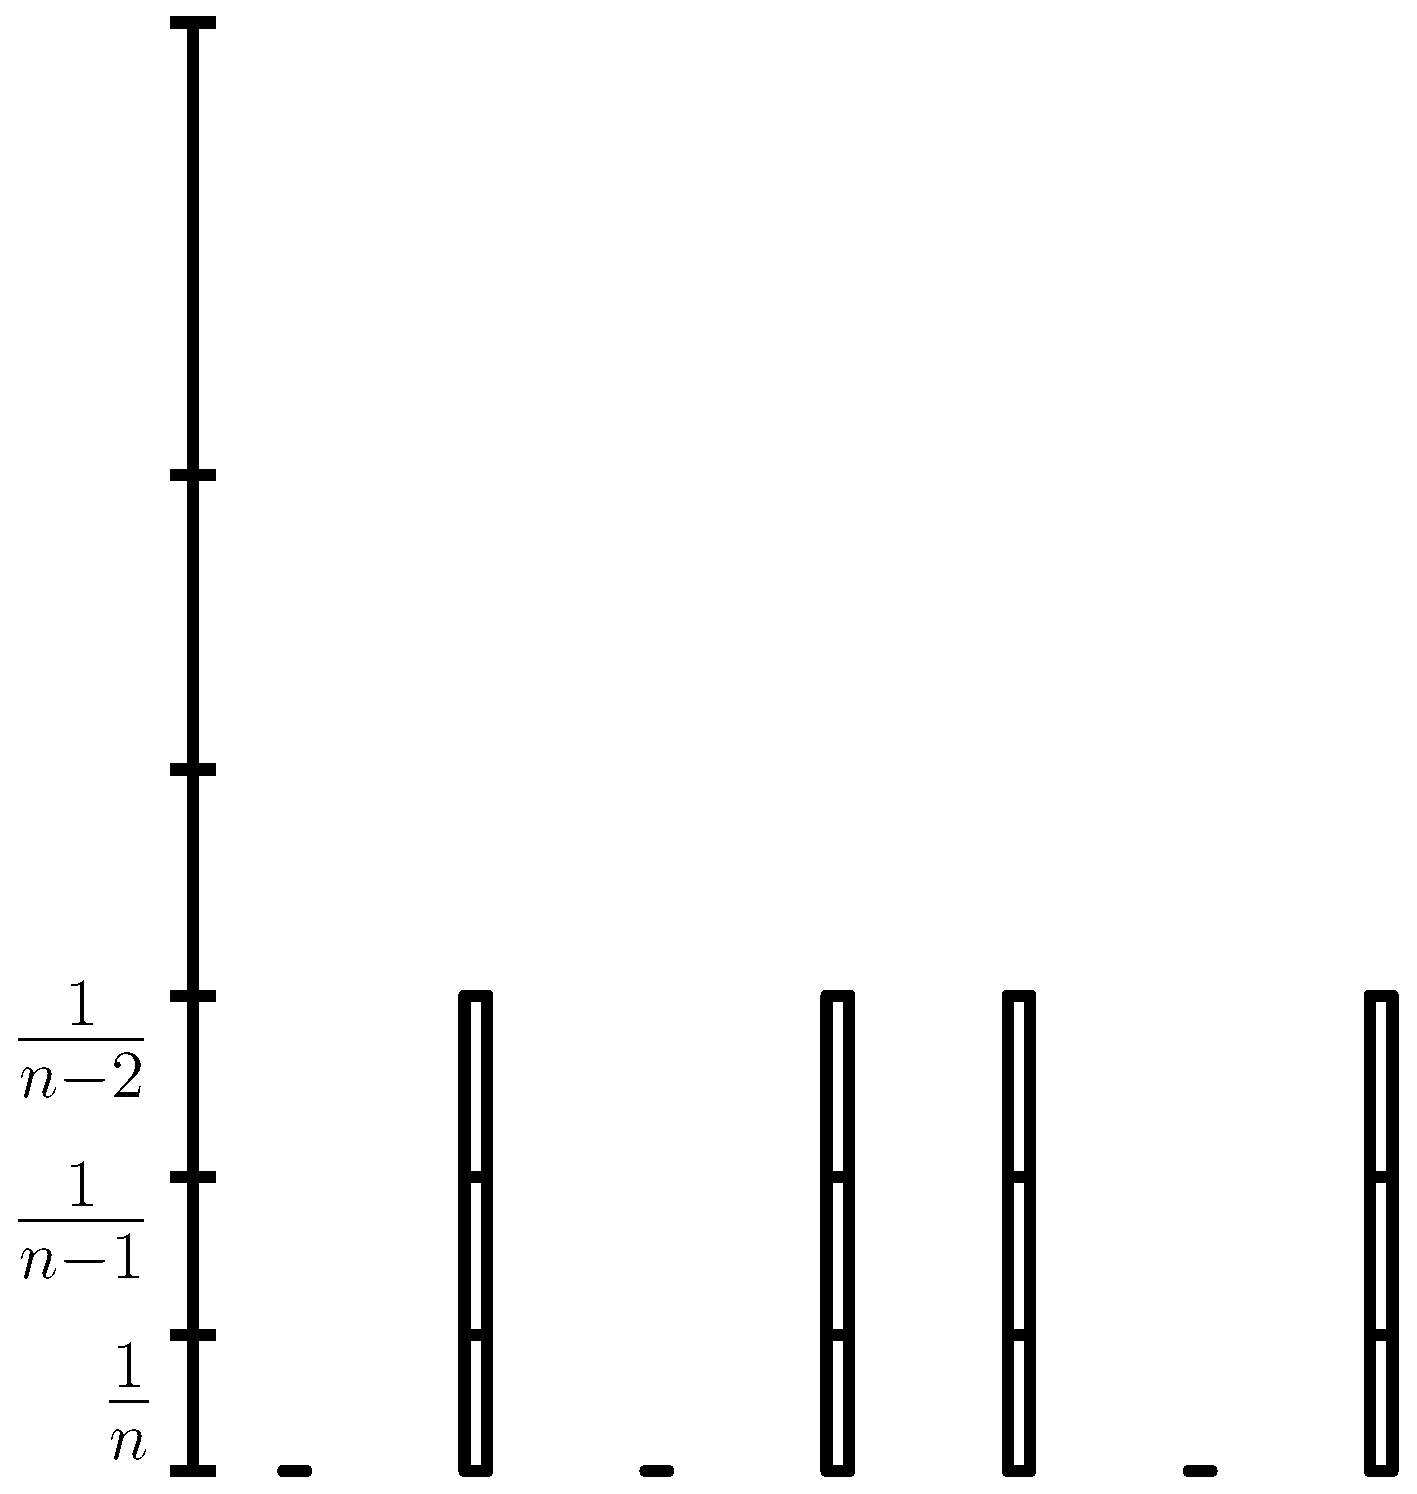
\includegraphics[width=0.5\linewidth]{singleProcessorLowerBound/round_3_1.eps}
    \onslide<8>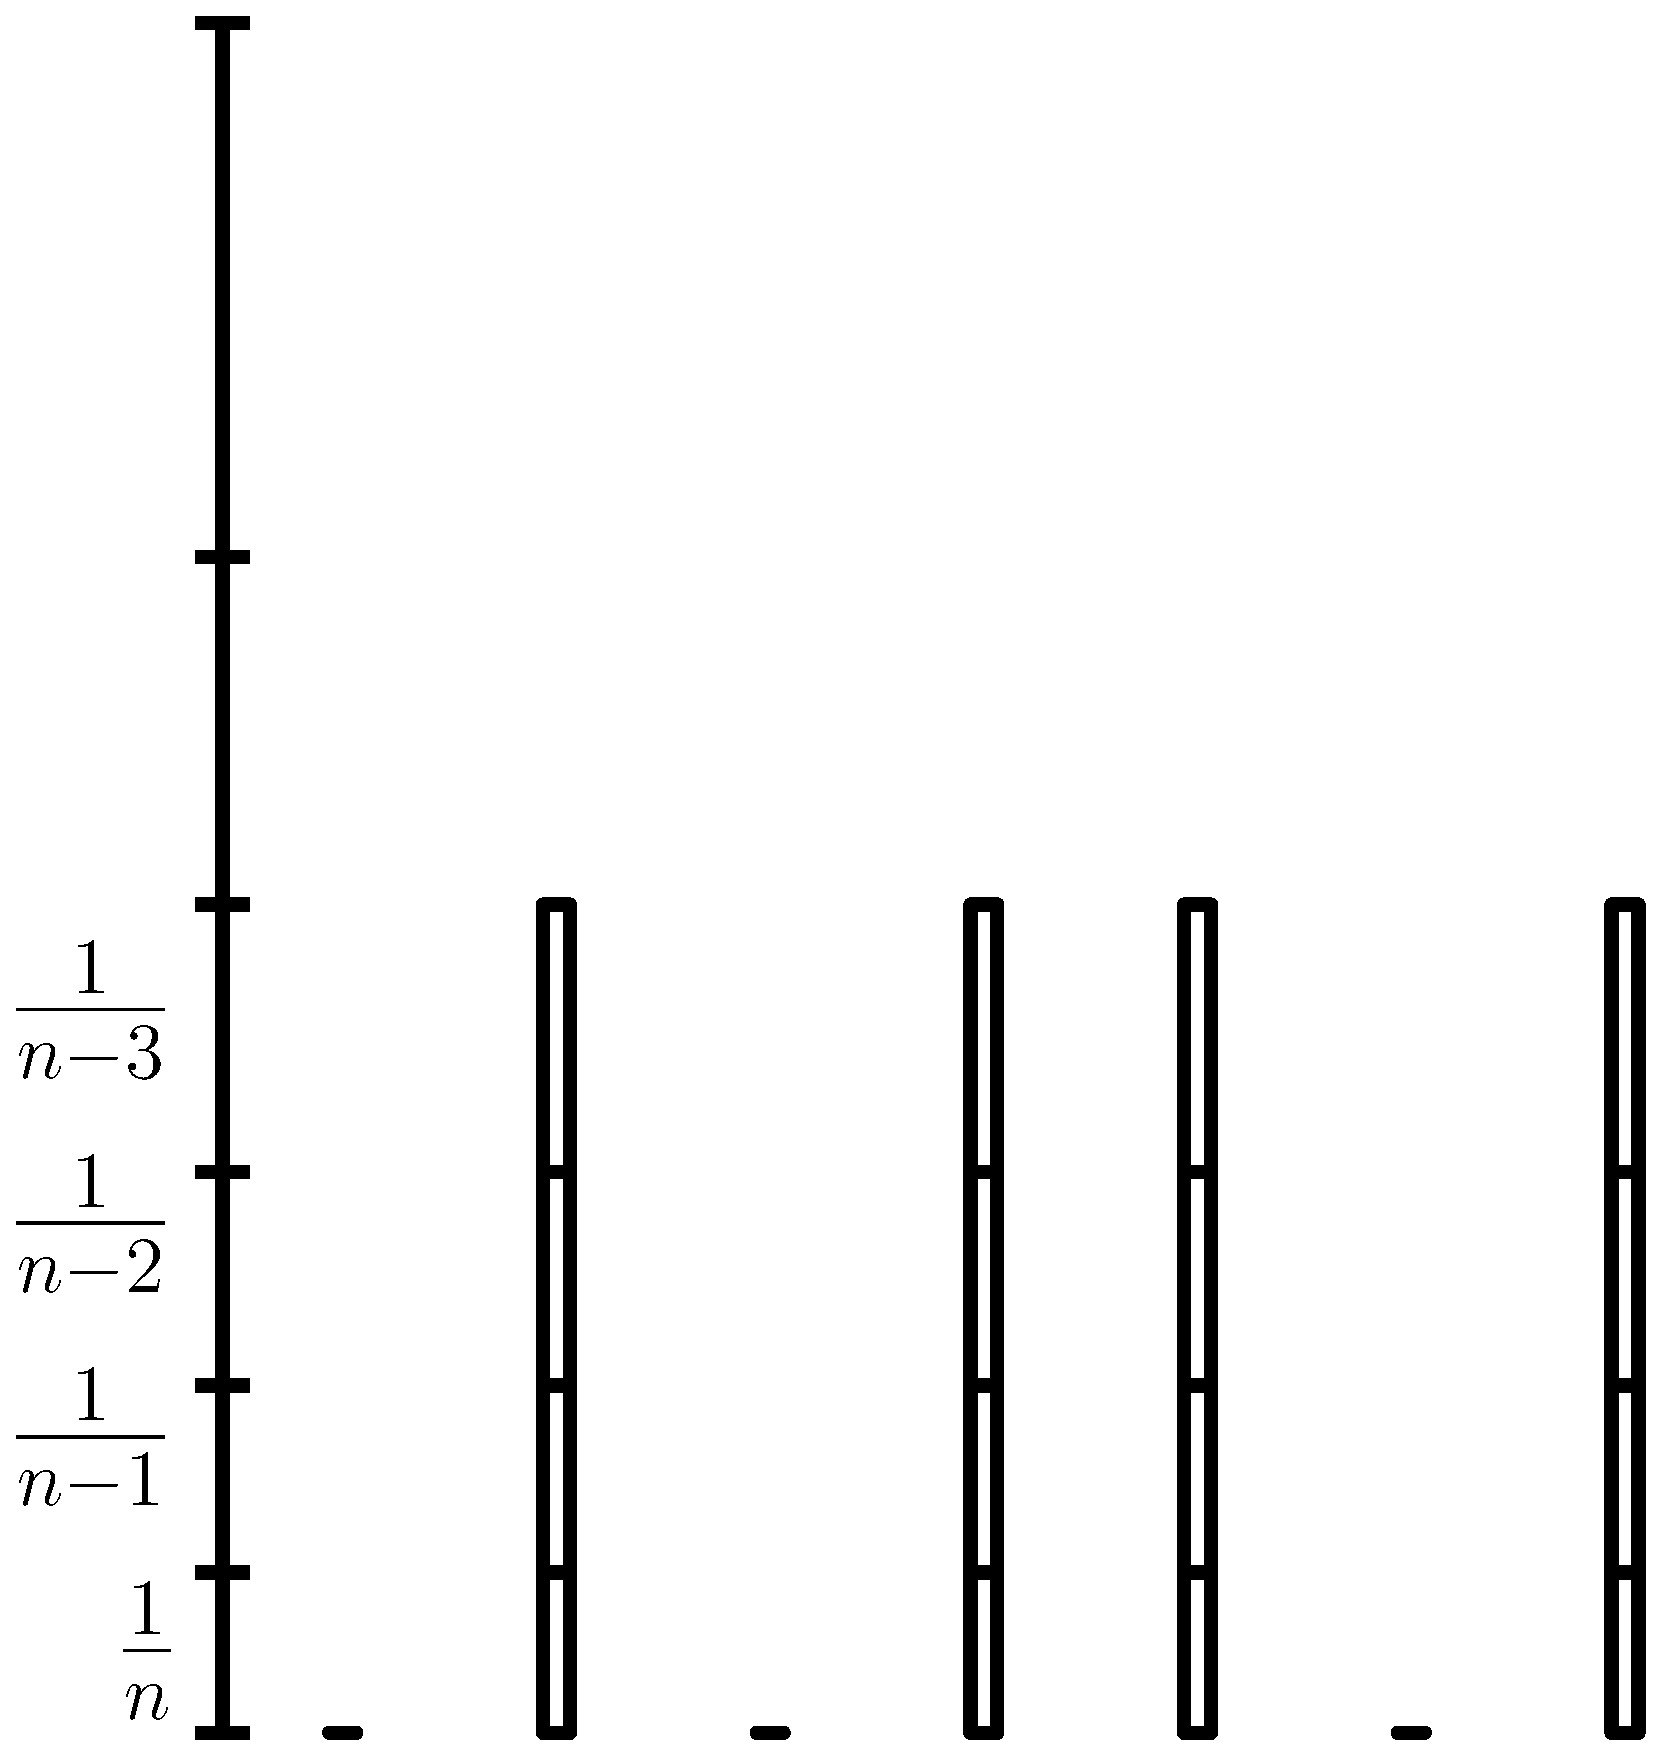
\includegraphics[width=0.5\linewidth]{singleProcessorLowerBound/round_4_0.eps}
    \onslide<9>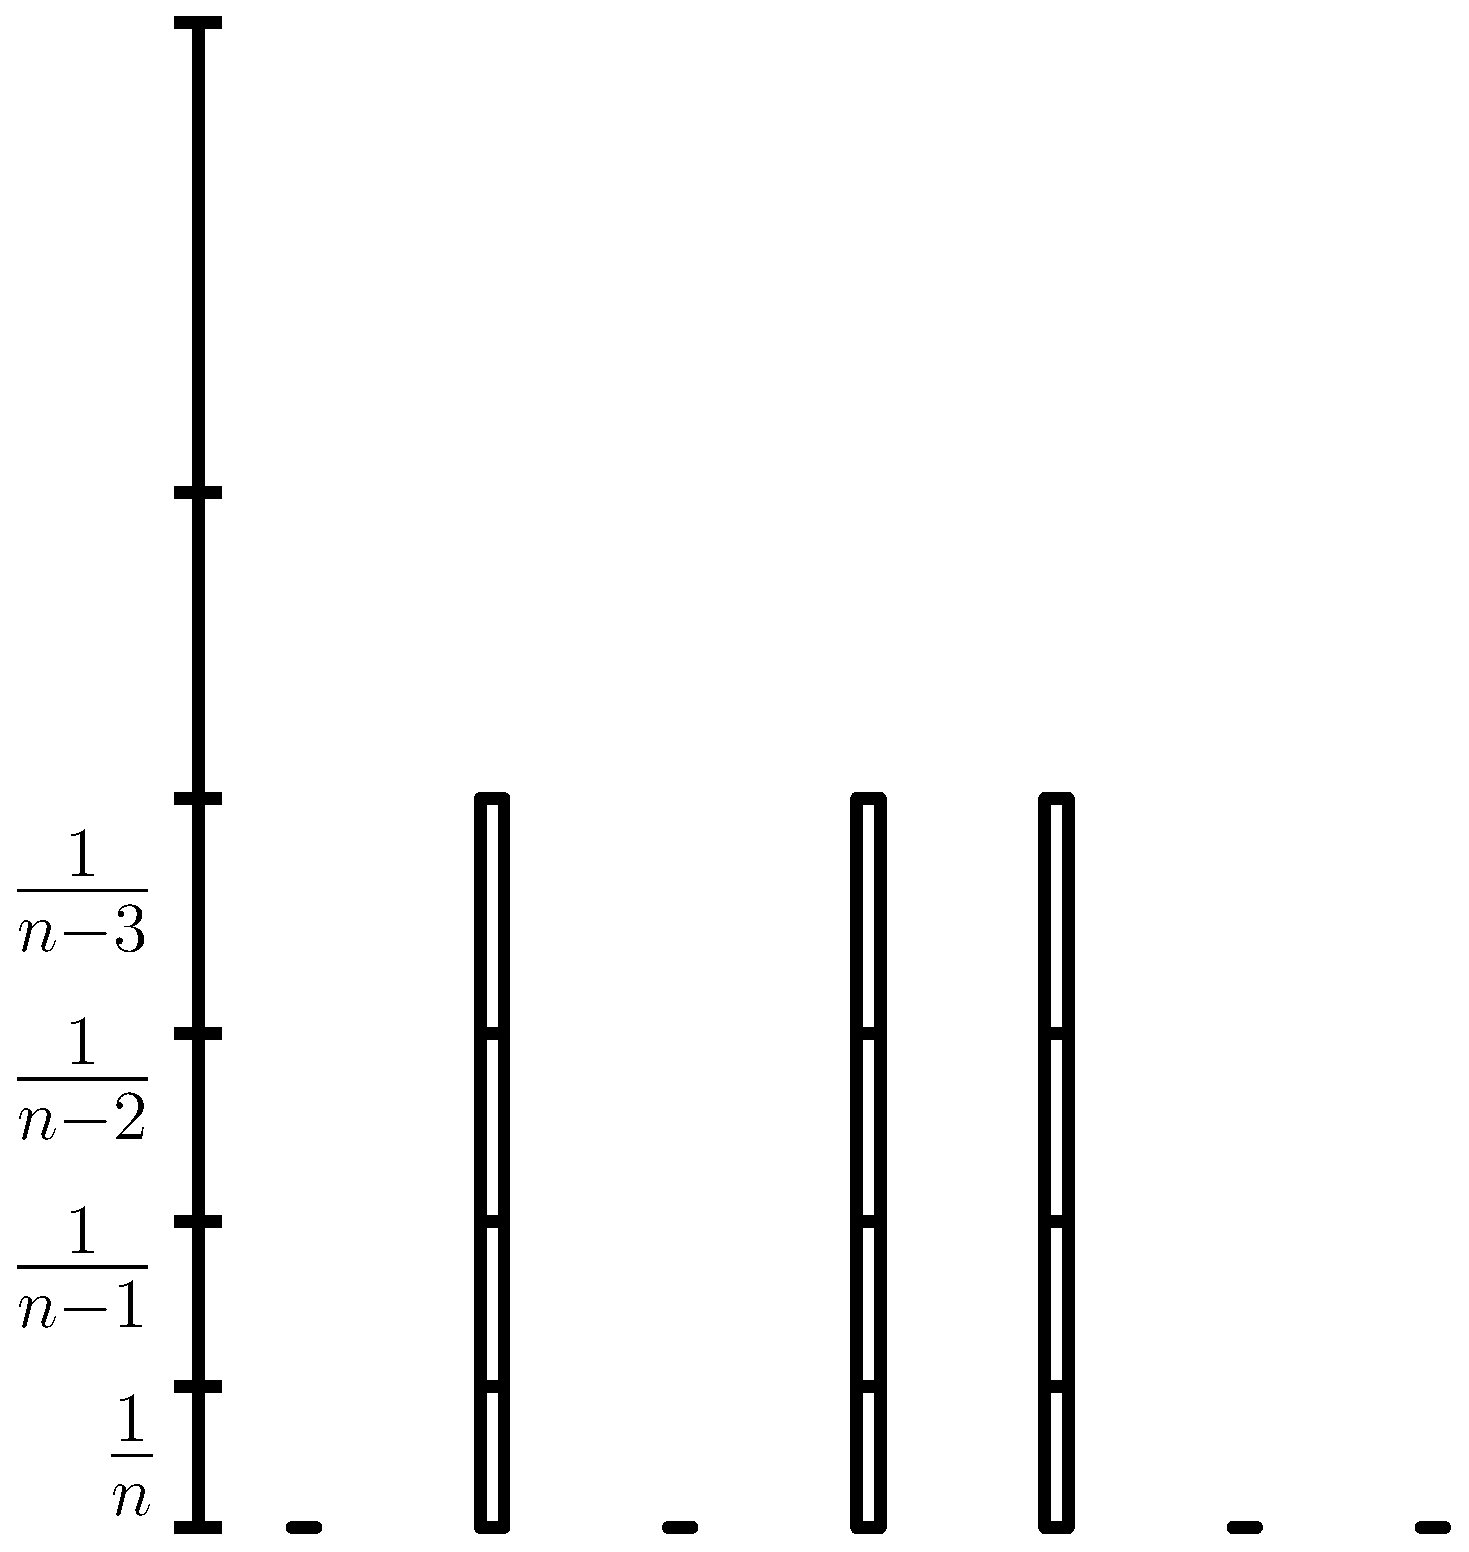
\includegraphics[width=0.5\linewidth]{singleProcessorLowerBound/round_4_1.eps}
    \onslide<10>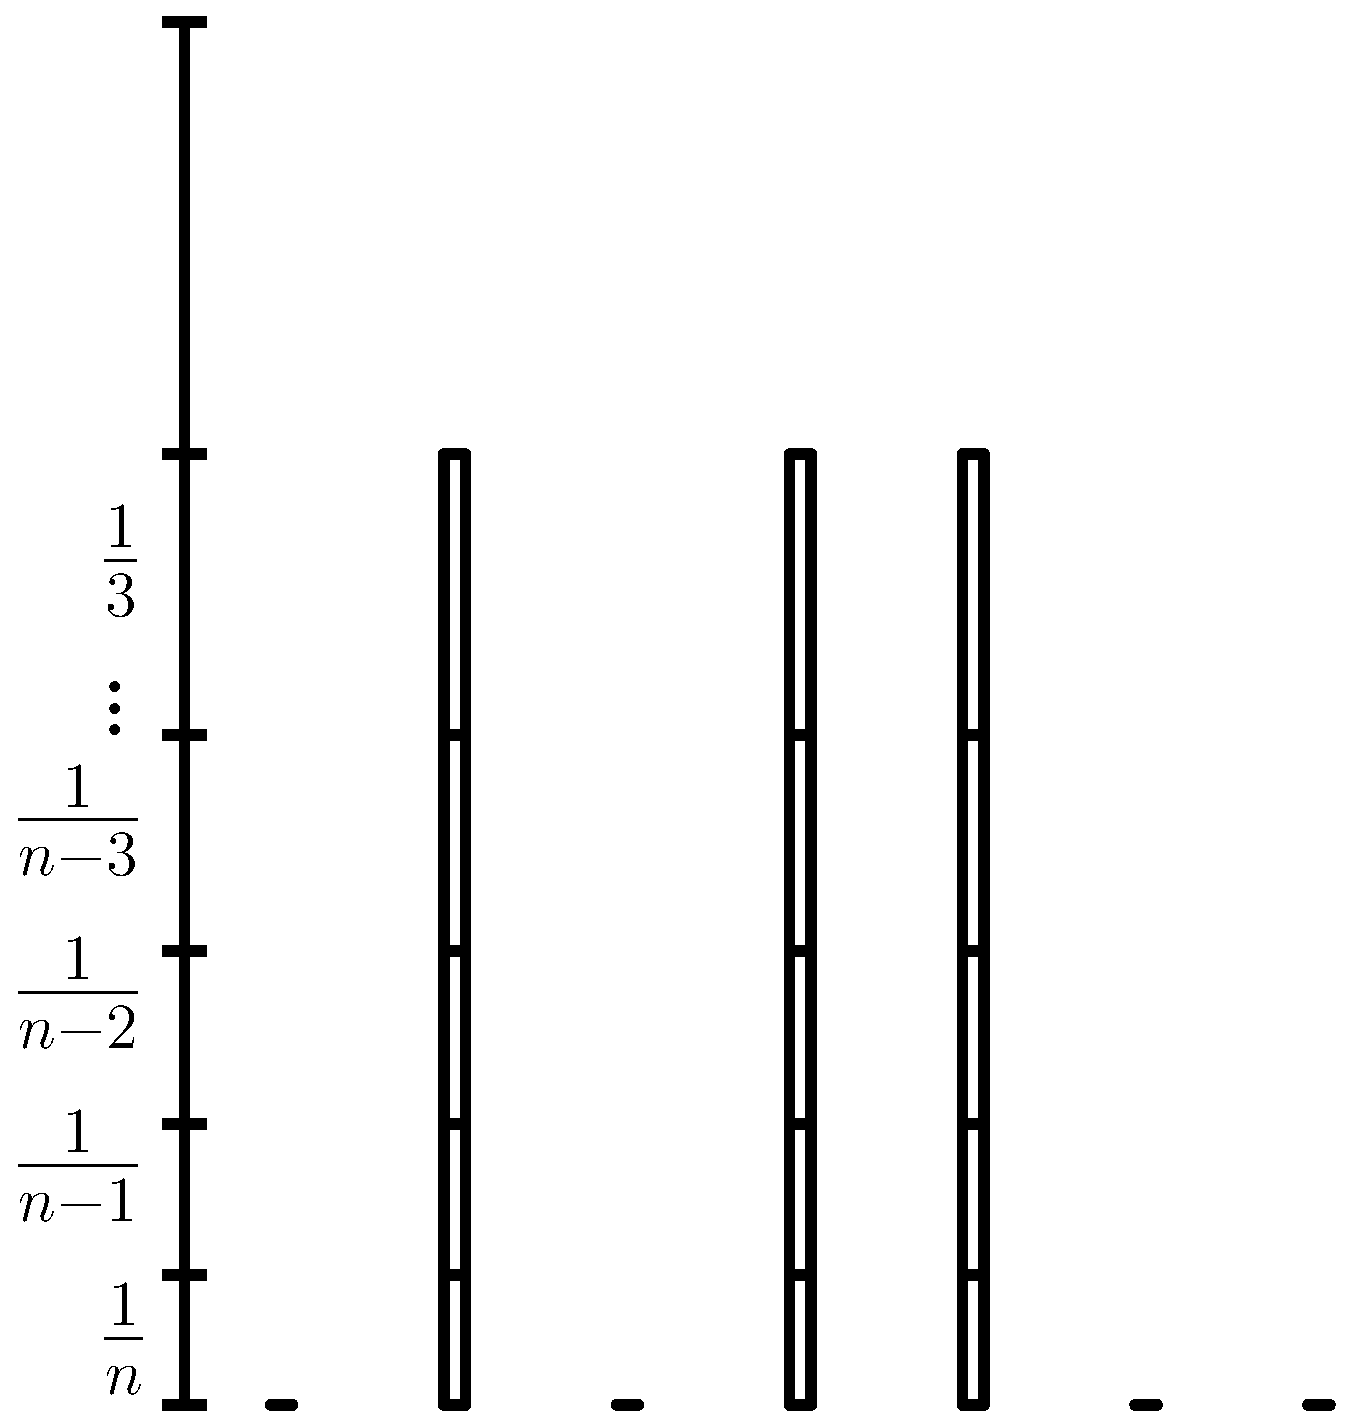
\includegraphics[width=0.5\linewidth]{singleProcessorLowerBound/round_5_0.eps}
    \onslide<11>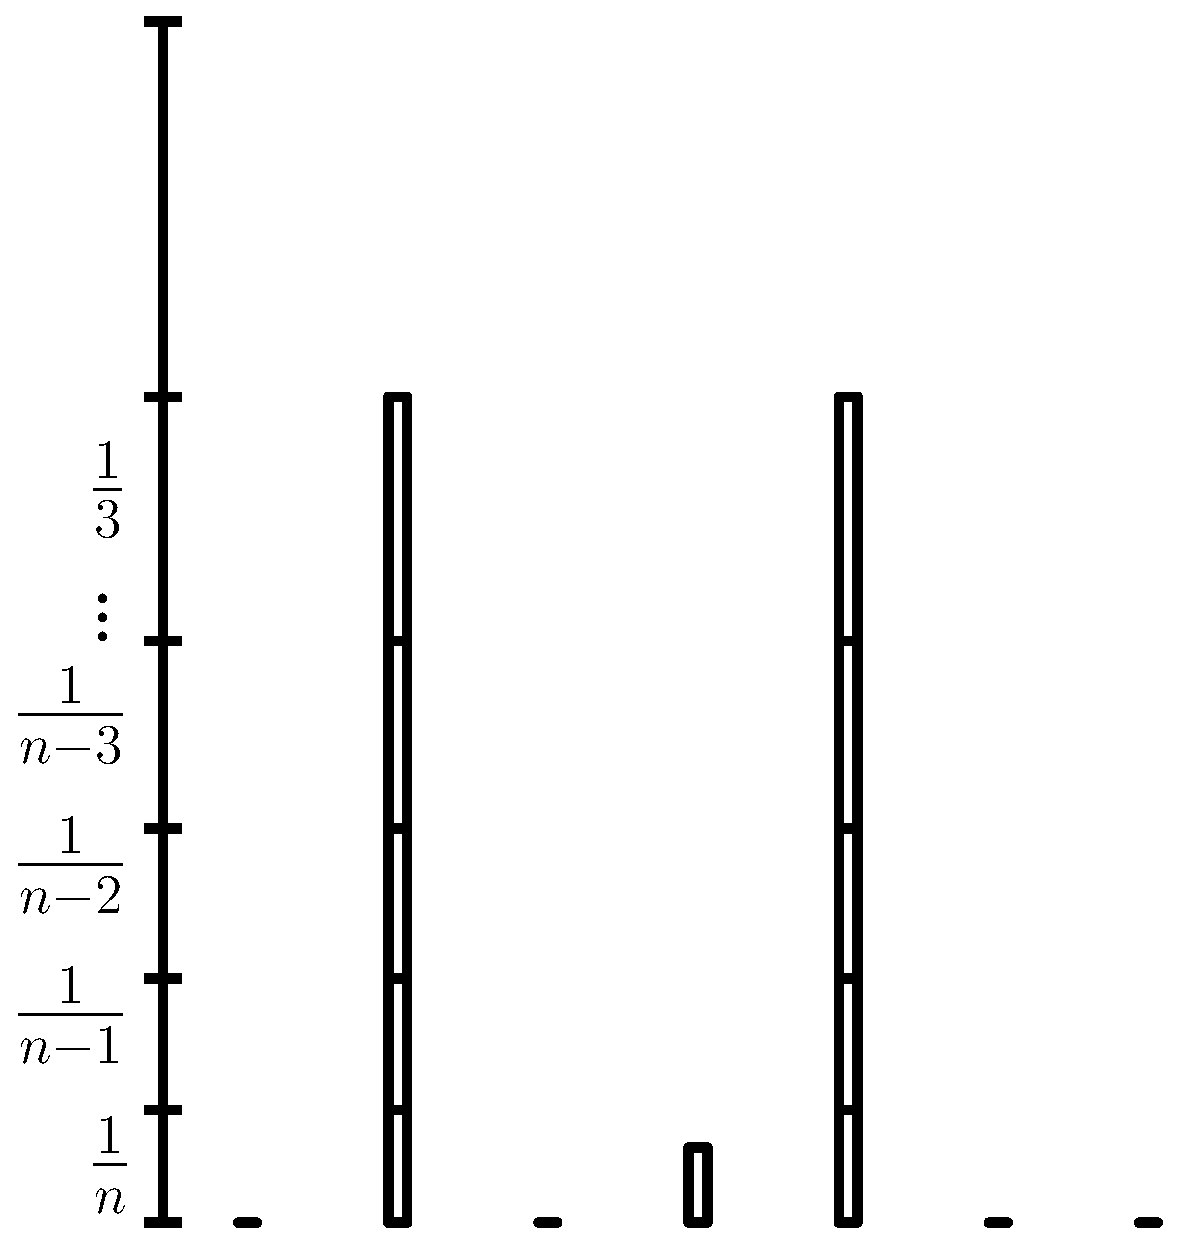
\includegraphics[width=0.5\linewidth]{singleProcessorLowerBound/round_5_1.eps}
    \onslide<12>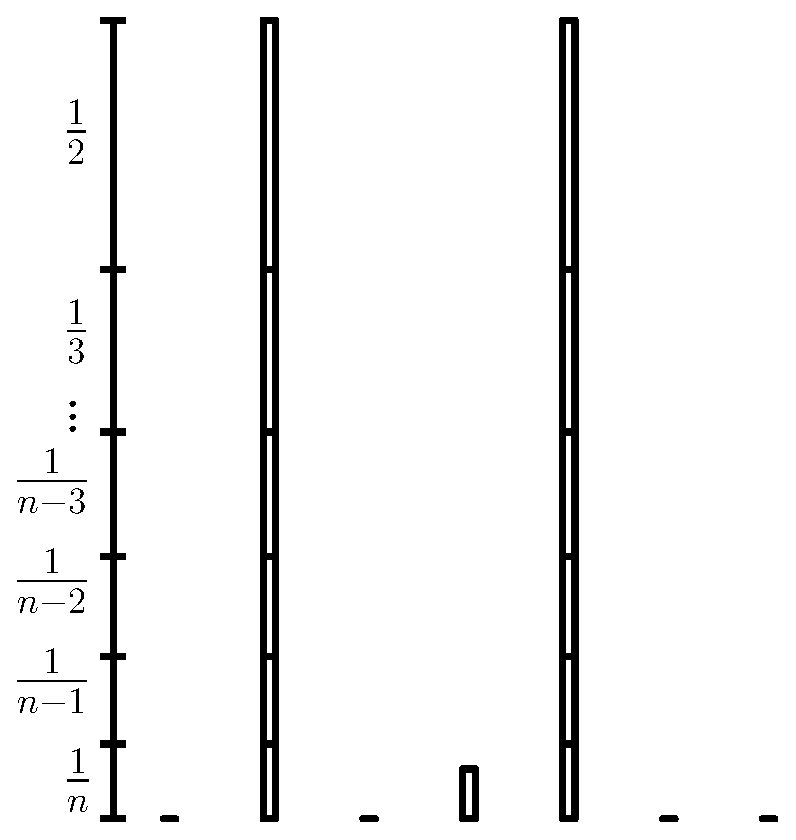
\includegraphics[width=0.5\linewidth]{singleProcessorLowerBound/round_6_0.eps}
    \onslide<13>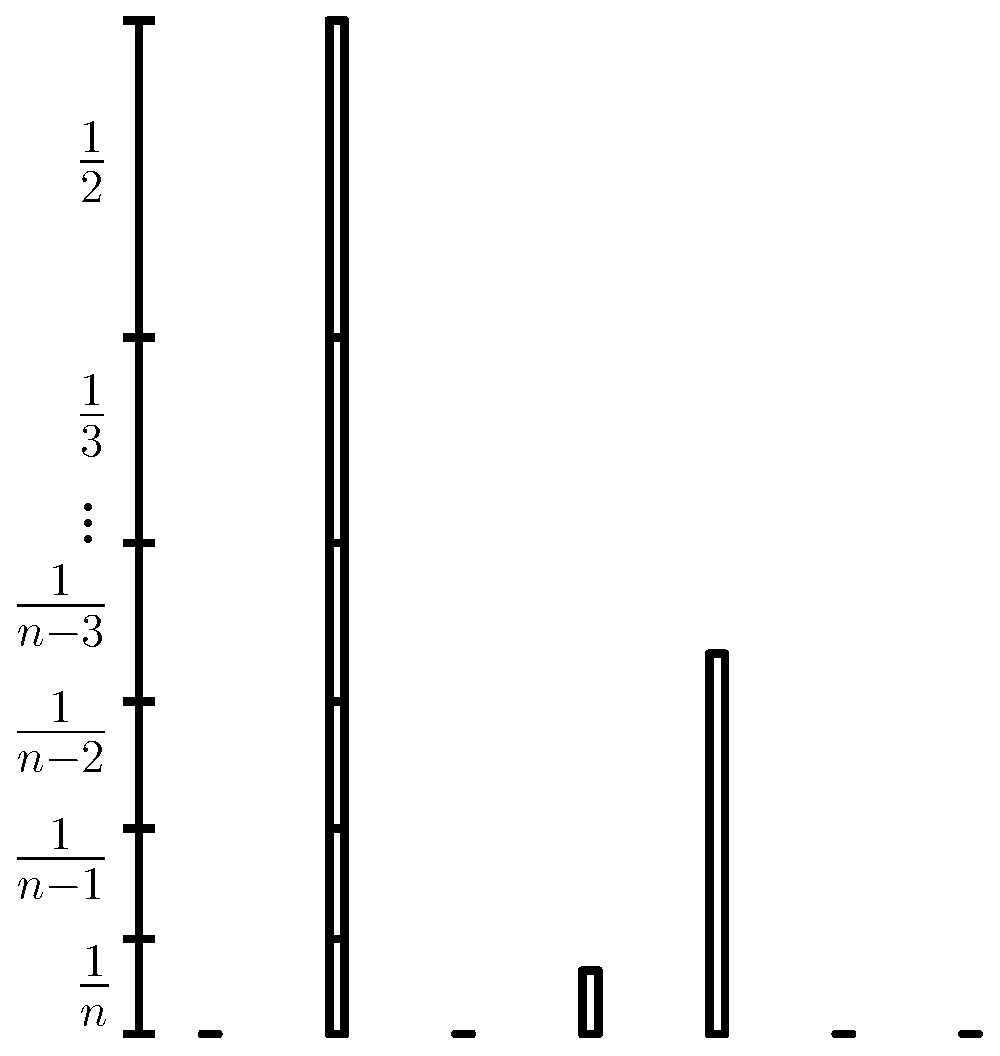
\includegraphics[width=0.5\linewidth]{singleProcessorLowerBound/round_6_1.eps}
    \onslide<14>\vspace{1.5cm}Achieves backlog: $$\frac{1}{n} + \frac{1}{n-1} + \cdots + \frac{1}{2} = \Omega(\log n).$$ 
  \end{overprint}
\end{frame}

\begin{frame}[t]{Single-Processor Upper Bound}
  A \defn{greedy emptier} -- an emptier that always empties from the
    fullest cup -- never lets backlog exceed $O(\log n)$.

  \vspace{0.75cm}
  \begin{definitions}
  \begin{itemize}
    \item $S_t$: state at start of round $t$
    \item $I_t$: state after the filler adds water on round $t$, but before the emptier removes water
    \item $\mu_k(S)$: average fill of $k$ fullest cups at state $S$.
  \end{itemize}
  \end{definitions}
\end{frame}

\begin{frame}[t]{Single-Processor Upper Bound Proof}
  \textbf{Proof:}
  Inductively prove a set of invariants: 
    $$\mu_k(S_t) \le \frac{1}{k+1} + \ldots +\frac{1}{n}.$$

  \vspace{0.25cm}
  Let $a$ be the cup that the emptier empties from on round $t$

  \vspace{0.25cm}
  \textbf{If $a$ is one of the $k$ fullest cups in $S_{t+1}$:}
  $$\mu_k(S_{t+1}) \le \mu_k(S_t).$$
  \textbf{Otherwise:}
  $$\mu_k(S_{t+1}) \le \mu_{k+1}(I_t) \le \mu_{k+1}(S_{t}) + \frac{1}{k+1}.$$
\end{frame}

\begin{frame}[t]{Previous work on Cup Games}
  \begin{itemize}
    \item The Single-Processor cup game ($p=1$) has been tightly analyzed with \defn{oblivious} and \defn{adaptive} fillers (i.e. fillers that can't and can observe the emptier's actions).
    \item The Multi-Processor cup game ($p>1$) is substantially more difficult. With an adaptive filler:
      \begin{itemize}
        \item Kuszmaul established upper bound of $O(\log n)$.\footnote{\tiny\color{blue}William Kuszmaul. Achieving optimal backlog in the vanilla multi-processor cup game. SIAM, 2020.}
        \item We established a matching lower bound of $\Omega(\log n)$.
      \end{itemize}
    \item The multi-processor cup game with an oblivious filler has not yet
      been tightly analyzed.
    \item Variants where valid moves depend on a graph have been studied.
    \item Variants with resource augmentation have been studied.
    \item Variants with semi-clairvoyance have been studied.
  \end{itemize}
\end{frame}

\begin{frame}[t]{Previous Work --- $p=1$}

  Single-processor cup game

  Adaptive filler:
  \begin{itemize}
    \item $\Omega(\log n)$ lower bound
    \item $O(\log n)$ upper bound
  \end{itemize}

  Oblivious filler (can't see emptier's actions):
  \footnote{[M. Bender, M. Farach-Colton, and W. Kuszmaul. Achieving optimal backlog in multi-processor cup games. In Proceedings of the 51st Annual ACM Symposium on Theory of Computing (STOC), 2019.]}
  \begin{itemize}
    \item $\Omega(\log\log n)$ lower bound
    \item $O(\log\log n)$ upper bound (with good probability in short games)
  \end{itemize}
\end{frame}

\begin{frame}[t]{Previous Work --- Restricted Versions}
  Cup flushing game (emptier can completely empty cups):\footnote{[P. F. Dietz and R. Raman. Persistence, amortization and randomization. In Proceedings of the Second An- nual ACM-SIAM Symposium on Discrete Algorithms (SODA), pages 78–88, 1991.]}
\begin{itemize}
  \item $\Omega(\log \log n)$ lower bound
  \item $O(\log \log n)$ upper bound
\end{itemize}

Bamboo Garden Trimming (filler always adds same amount):\footnote{[Bilò, Davide, Luciano Gualà, Stefano Leucci, Guido Proietti, and Giacomo Scornavacca. "Cutting Bamboo Down to Size." arXiv preprint arXiv:2005.00168 (2020).]}
\begin{itemize}
  \item $2$ lower bound
  \item $2$ upper bound
\end{itemize}

Cups are nodes in a graph, moves restricted based on graph structure. $D$ is the diameter of the graph.
\begin{itemize}
  \item $\Omega(D)$ lower bound
  \item $O(D)$ upper bound
\end{itemize}
\end{frame}


\begin{frame}[t]{Our Variant}
  \begin{definition}
    \defn{Variable-Processor Cup Game}: \\
    Each round filler can change $p$ 
  \end{definition}

\vspace{1cm}
Modification may seem small, but it drastically
alters the game!

\end{frame}

\begin{frame}[c]{}
\begin{center}
\Huge Adaptive Filler\\ Lower Bound
\end{center}
\end{frame}

\begin{frame}[t]{Negative Fill}
  In lower bound proofs we allow \defn{negative fill}
  \begin{itemize}
    \item Measure fill relative to average fill
    \item Important for recursion 
    \item Strictly easier for the filler if cups can zero out
  \end{itemize}
\end{frame}

\begin{frame}[t]{Amplification Lemma}
  \begin{lemma}
    Given a strategy for achieving backlog $f(n)$ on $n$ cups, we can construct a new strategy that achieves backlog 
    $$f'(n) \ge (1-\delta)\sum_{\ell=0}^L f((1-\delta)\delta^\ell n)$$
    for appropriate parameters $L\in\mathbb{N}, 0<\delta\ll 1/2$.
  \end{lemma}
\end{frame}

\begin{frame}[t]{Amplification Lemma Proof Sketch}
  \begin{itemize}
    \item $A$ starts as the $\delta n$ fullest cups, $B$ as the $(1-\delta)n$ other cups.
    \item Repeatedly apply $f$ to $B$ and swap generated cup into $A$. 
    \item Decrease $p$, recurse on $A$.
  \end{itemize} 
  \vspace{0.5cm}
  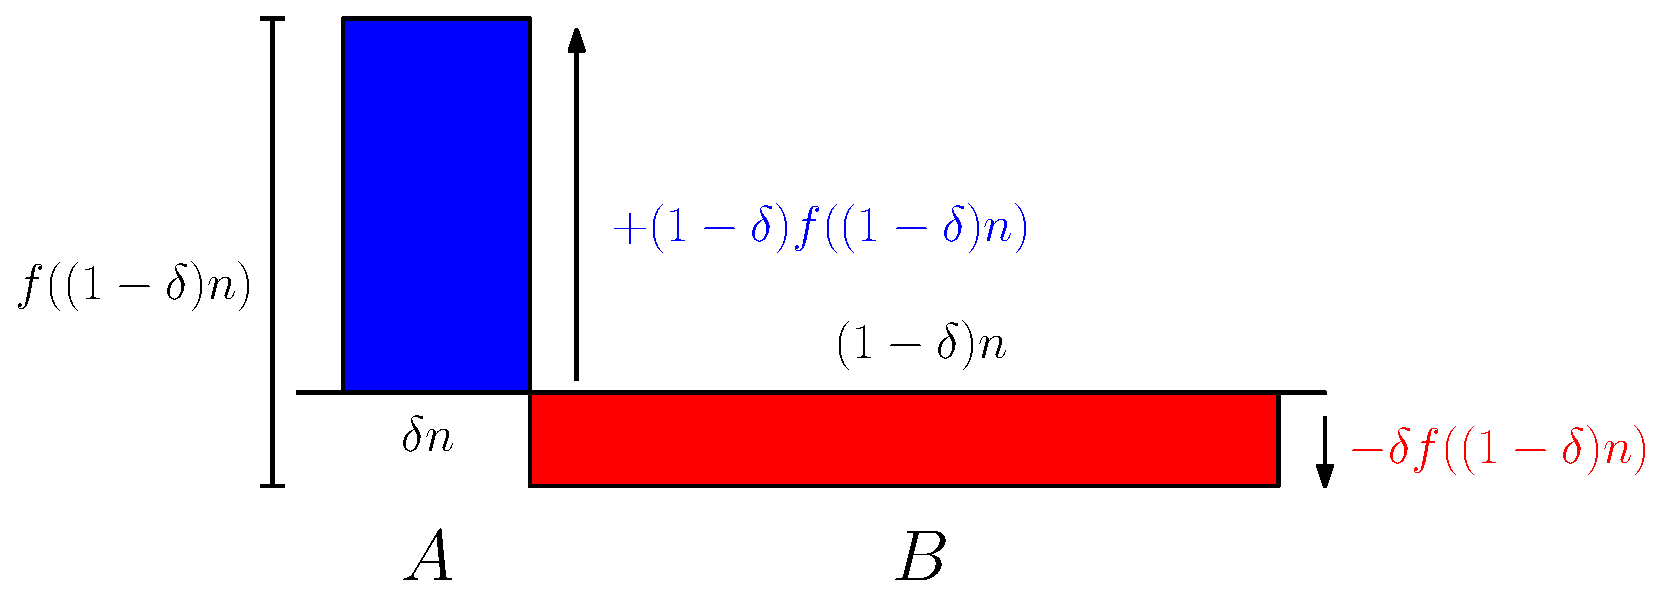
\includegraphics[width=\linewidth]{amplificationImgs/delta_one_minus_delta.eps}
\end{frame}

\begin{frame}[t]{Adaptive Filler Lower Bound}
  Let $\epsilon > 0$ be any constant. Then there is some $\delta=\Theta(1)$ such that by repeated amplification we get: 
  \begin{theorem}
    There is an adaptive filling strategy that achieves
    backlog $\Omega(n^{1-\epsilon})$  in running-time $2^{O(\log^2 n)}$.
  \end{theorem}
  \vspace{0.5cm}
  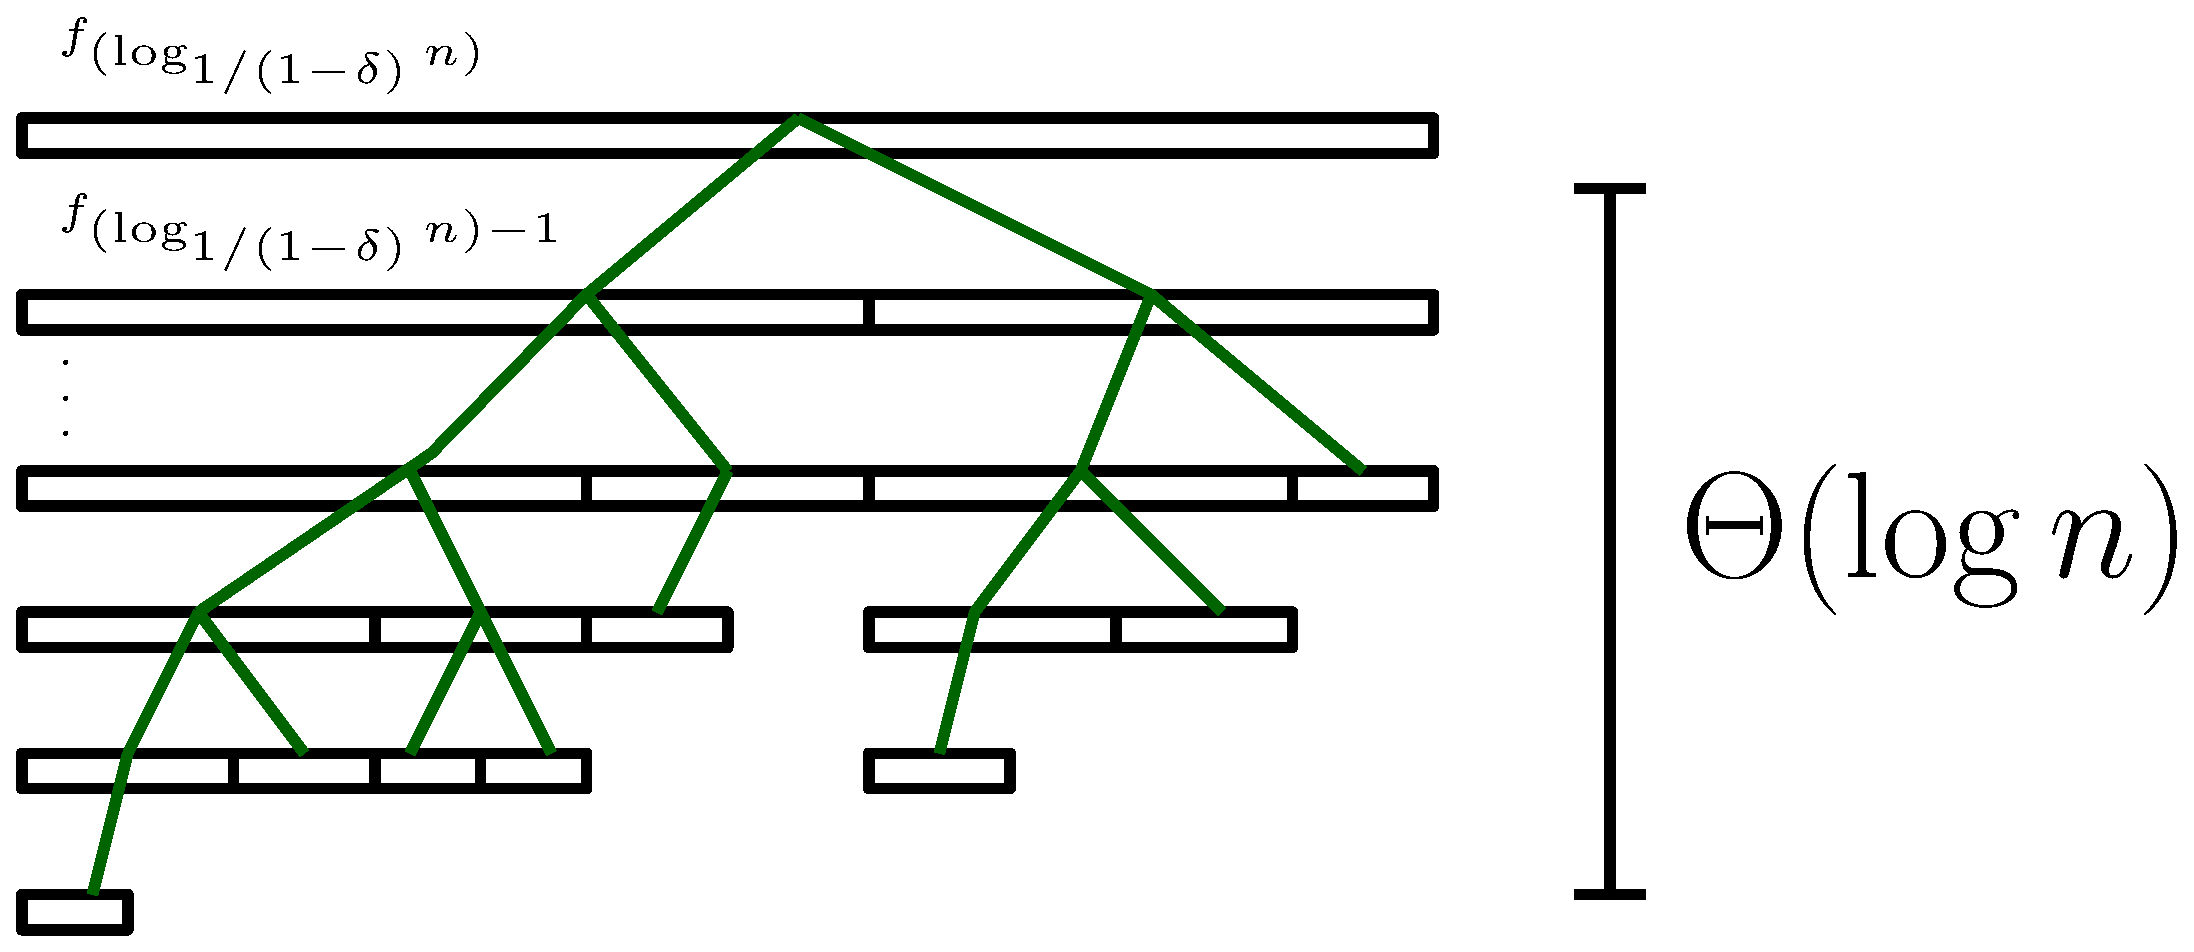
\includegraphics[width=0.7\linewidth]{amplificationImgs/quasipoly_cor.eps}
\end{frame}

\begin{frame}[t]{Adaptive Filler Lower Bound}
  Extremal strategy:\\
  By repeated amplification using $\delta=\Theta(1/n)$ we get: 
  \begin{theorem}
    There is an adaptive filling strategy that achieves backlog $\Omega(n)$ in running-time $O(n!)$.
  \end{theorem}
  \vspace{0.5cm}
  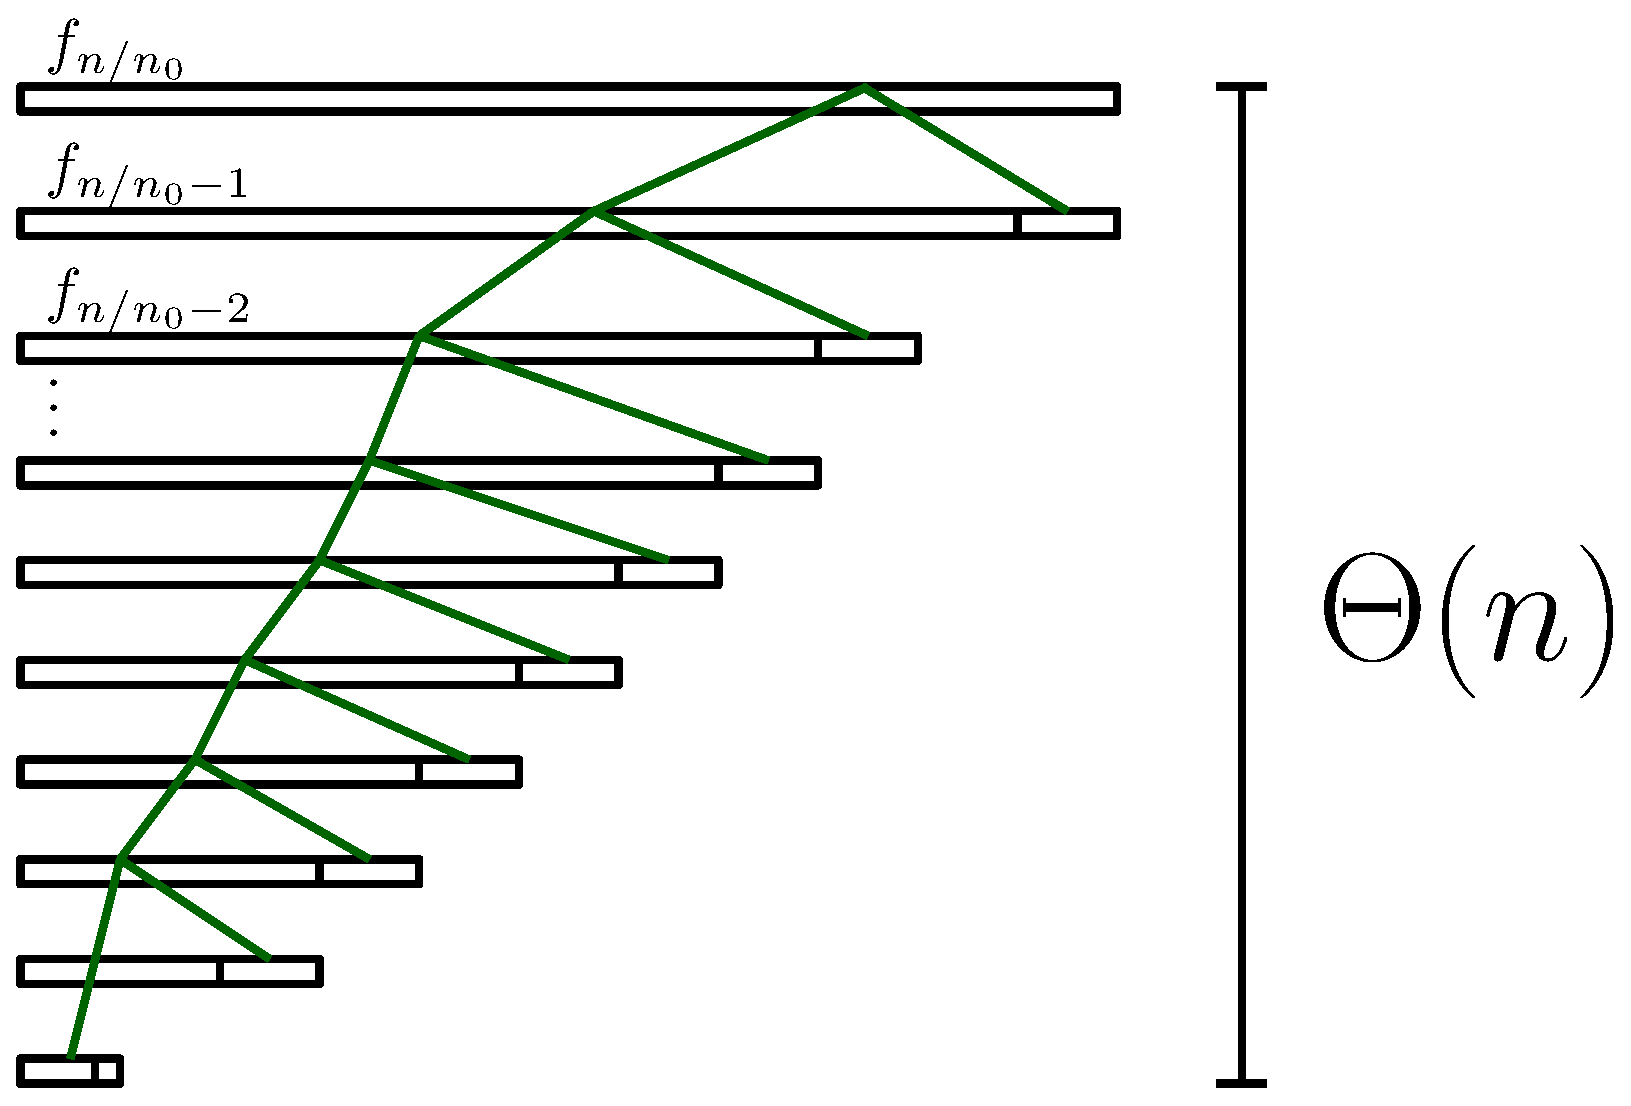
\includegraphics[width=0.45\linewidth]{amplificationImgs/expo_cor.eps}
\end{frame}

\begin{frame}[c]{}
  \begin{center}
    \Huge Upper Bound 
  \end{center}
\end{frame}

\begin{frame}[t]{Upper Bound}
  We prove a novel set of invariants:

  \begin{theorem}
    A greedy emptier maintains the invariant:
    $$\mu_k(S_t) \le 2n-k.$$
  \end{theorem}

  \begin{corollary}
  A greedy emptier never lets backlog exceed $$O(n).$$
  \end{corollary}

  \vspace{0.3cm}
  Note: this matches our lower bound!
\end{frame}

\begin{frame}[t]{Upper Bound Proof Sketch}
  Induct on $t$. Fix $k$. Define sets of cups:\\
  \begin{itemize}
    \item $A$: (emptied from) $\cap$ ($k$ fullest in $S_t$) $\cap$ ($k$ fullest in $S_{t+1}$)
    \item $B$: (emptied from) $\cap$ ($k$ fullest in $S_t$) $\cap$ (\textbf{not} $k$ fullest in $S_{t+1}$)
    \item $C$: $AC$ is the $k$ fullest cups in $S_{t+1}$
  \end{itemize}
  $\mu_k(S_{t+1})$ is largest if fill from $BC$ is pushed into $A$

  \vspace{0.25cm}
  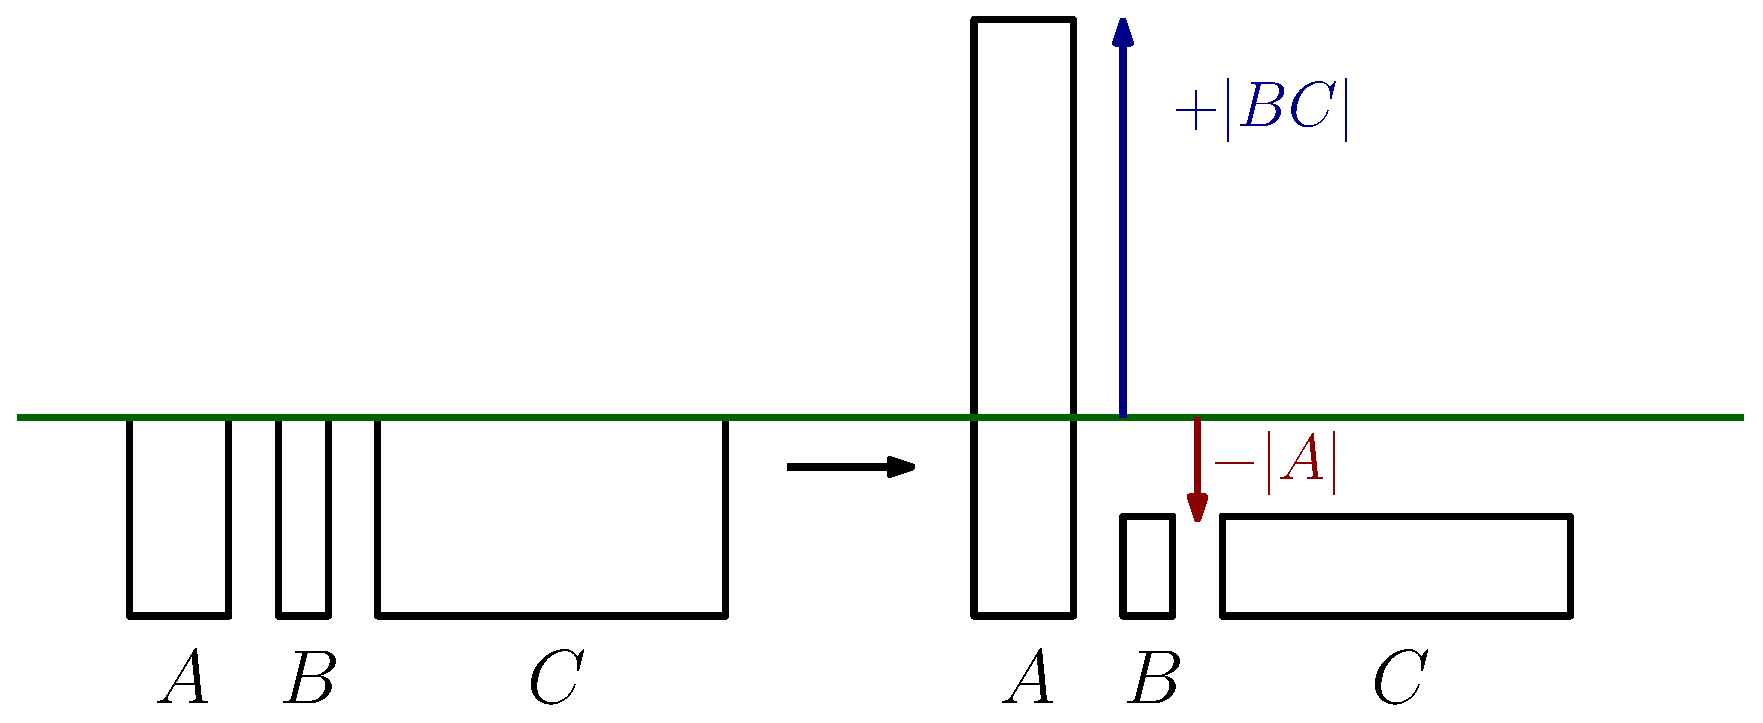
\includegraphics[width=\linewidth]{upperbound/upperboundpf.eps}
\end{frame}

\begin{frame}[c]{}
  \begin{center}
    \Huge Oblivious Filler \\
    Lower Bound
  \end{center}
\end{frame}

\begin{frame}[t]{Oblivious Filler Lower Bound}
  \begin{definition}
    \defn{Oblivious Filler:}
    Can't observe the emptier's actions 
  \end{definition}

  \begin{itemize}
    \item Classically emptier does better in the randomized setting.
    \item But not in the variable-processor cup game!
    \item We get the same lower bound as with an adaptive filler in quasi-polynomial length games!
  \end{itemize}

  % In the variable-processor cup game--shockingly--an oblivious filler can
  % achieve an identical lower bound for games of length $2^{\polylog(n)}$ 
  % with probability at least $1-2^{-\polylog(n)}$, although only against \defn{greedy-like} emptiers.
\end{frame}

\begin{frame}[t]{Oblivious Filler Lower Bound}
  \begin{definition}
    $\Delta$-\defn{greedy-like} emptier: \\
    Let $x,y$ be cups. If $\text{fill}(x) > \text{fill}(y) + \Delta$ then a
    $\Delta$-greedy-like emptier empties from $y$ \emph{only if} it also
    empties from $x$.
  \end{definition}

  \vspace{0.5cm}
  Oblivious filler can achieve backlog $\Omega(n^{1-\epsilon})$ for $\epsilon
  >0 $ constant in running time $2^{\polylog(n)}$ against a
  $\Delta$-greedy-like emptier ($\Delta \le O(1)$) with probability at least
  $1-2^{-\polylog(n)}$.

\end{frame}

\begin{frame}[t]{Flattening}
 \begin{definition}
   A cup configuration is $R$-flat if all cups have fills in $[-R, R]$.
 \end{definition} 
 \vspace{1cm}
 \begin{proposition} 
   Oblivious filler can get a $2(2+\Delta)$-flat configuration from an
   $R$-flat configuration against a $\Delta$-greedy-like emptier in running
   time $O(R)$.
 \end{proposition}
\end{frame}

\begin{frame}[t]{Oblivious Filler: Constant Fill}
  Getting constant fill in a \emph{known} cup is hard now. Strategy:
  \begin{itemize}
    \item Play many single-processor cup games on $\Theta(1)$ cups
      blindly. Each succeeds with constant probability.
    \item By a Chernoff Bound with probability $1-2^{-\Omega(n)}$ at least a constant fraction $nc$ of these succeed.
    \item Set $p=nc$.
    \item Fill $nc$ known cups; because emptier is greedy-like it must focus on the $nc$ cups with high fill before these cups.
    \item Recurse on the $nc$ known cups with high fill.
  \end{itemize}
\end{frame}

\begin{frame}[t]{Oblivious Amplification Lemma}
Almost identical to the Adaptive Amplification Lemma!
  \begin{lemma}
    Given a strategy $f$ for achieving backlog $f(n)$ on $n$ cups, we can construct a new strategy that achieves backlog 
    $$f'(n) \ge \phi \cdot (1-\delta)\sum_{\ell=0}^L f((1-\delta)\delta^\ell n)$$
    for appropriate parameters $L\in\mathbb{N}, 0<\delta\ll 1/2$ and constant $\phi \in (0,1)$ of our choice against a greedy-like emptier.
  \end{lemma}

  (Note: Lemma is actually more complicated than this.)
\end{frame}

\begin{frame}[t]{Oblivious Filler Lower Bound }
  \begin{theorem}
    There is an oblivious filling strategy that achieves backlog
    $$\Omega(n^{1-\epsilon})$$ for constant $\epsilon > 0$ with probability at
    least $1-2^{-\polylog(n)}$ in running time $2^{O(\log^2 n)}$ against a greedy-like emptier.
  \end{theorem}

  Achieve this probability by a union bound on $2^{\polylog(n)}$ events.

  \vspace{0.5cm}
  Proof notes: 
  \begin{itemize}
    \item Similar to adaptive filler proof
    \item need larger base case for union bound to work; this doesn't harm backlog though
  \end{itemize}
\end{frame}

\end{document}
